\documentclass[11pt,oneside]{article}
\usepackage[a4paper,margin=26mm,headheight=15pt]{geometry}
\usepackage[T1]{fontenc}
\usepackage[utf8]{inputenc}
\IfFileExists{libertinus.sty}{\usepackage{libertinus}}{\usepackage{lmodern}}
\usepackage{microtype}
\usepackage{amsmath,amssymb,amsthm,mathtools,mathrsfs,bm}
\usepackage{booktabs,longtable,array,tabularx,multirow}
\usepackage{graphicx}
\usepackage{caption}
\usepackage{xcolor}
\usepackage{enumitem}
\usepackage{fancyhdr}
\usepackage{titlesec}
\usepackage{listings}
\usepackage{xurl}
\usepackage[hypertexnames=false]{hyperref}
\usepackage[nameinlink,noabbrev]{cleveref}

\graphicspath{
  {assets/fabius_dyadic_interpolation_report/figures/}
  {assets/fabius_interpolation_report/figures/}
  {assets/Fabius_Rvachev_Dyadic_Interpolation_Report/figures/}
}

\definecolor{linkblue}{RGB}{25,75,135}
\definecolor{deepgreen}{RGB}{28,103,76}
\definecolor{shadegray}{RGB}{246,247,249}
\definecolor{rulegray}{RGB}{195,201,208}
\hypersetup{
  colorlinks=true,
  linkcolor=linkblue,
  citecolor=deepgreen,
  urlcolor=linkblue,
  pdftitle={Dyadic-Comb Frontiers for the Fabius--Rvachev System},
  pdfsubject={Comb sums, exact Euler--Maclaurin collapse, spectral Dirichlet values,
    shifted quadrature, and global polynomial interpolation on the dyadic comb},
  pdfkeywords={Fabius function, Rvachev up-function, dyadic comb, Thue-Morse,
    Euler-Maclaurin, Hurwitz zeta, Bell polynomial, Bernoulli number, Runge phenomenon,
    Hermite interpolation, Lebesgue constant, Lambert W}
}

\pagestyle{fancy}
\fancyhf{}
\fancyhead[L]{\small Dyadic-comb frontiers}
\fancyhead[R]{\small\nouppercase{\leftmark}}
\fancyfoot[C]{\thepage}
\renewcommand{\headrulewidth}{0.4pt}
\titleformat{\section}{\Large\bfseries}{\thesection}{0.7em}{}
\titleformat{\subsection}{\large\bfseries}{\thesubsection}{0.7em}{}
\titleformat{\subsubsection}{\normalsize\bfseries}{\thesubsubsection}{0.7em}{}
\setcounter{secnumdepth}{3}
\setcounter{tocdepth}{2}
\setlist[itemize]{leftmargin=2em,itemsep=0.25em,topsep=0.4em}
\setlist[enumerate]{leftmargin=2.3em,itemsep=0.25em,topsep=0.4em}
\setlength{\emergencystretch}{3em}
\allowdisplaybreaks[2]
\numberwithin{equation}{section}

% ed.: shared-counter environments now use alias counters (aliascnt) so
% cleveref prints each environment's own name; with the plain
% \newtheorem{lemma}[theorem]{Lemma} pattern every \cref rendered as
% "theorem", even for lemmas, corollaries, and remarks.
\usepackage{aliascnt}
\newcommand{\newsharedtheorem}[2]{%
  \newaliascnt{#1}{theorem}%
  \newtheorem{#1}[#1]{#2}%
  \aliascntresetthe{#1}%
}
\newtheorem{theorem}{Theorem}[section]
\newsharedtheorem{proposition}{Proposition}
\newsharedtheorem{lemma}{Lemma}
\newsharedtheorem{corollary}{Corollary}
\newsharedtheorem{identity}{Identity}
\newsharedtheorem{conjecture}{Conjecture}
\newsharedtheorem{problem}{Problem}
\newsharedtheorem{question}{Research question}
\theoremstyle{definition}
\newsharedtheorem{definition}{Definition}
\newsharedtheorem{algorithm}{Algorithm}
\newsharedtheorem{example}{Example}
\newsharedtheorem{observation}{Numerical observation}
\theoremstyle{remark}
\newsharedtheorem{remark}{Remark}
\newsharedtheorem{warning}{Warning}
\crefname{conjecture}{conjecture}{conjectures}
\Crefname{conjecture}{Conjecture}{Conjectures}
\crefname{problem}{problem}{problems}
\Crefname{problem}{Problem}{Problems}
\crefname{question}{research question}{research questions}
\Crefname{question}{Research question}{Research questions}
\crefname{observation}{numerical observation}{numerical observations}
\Crefname{observation}{Numerical observation}{Numerical observations}
\crefname{identity}{identity}{identities}
\Crefname{identity}{Identity}{Identities}
\crefname{algorithm}{algorithm}{algorithms}
\Crefname{algorithm}{Algorithm}{Algorithms}
\crefname{warning}{warning}{warnings}
\Crefname{warning}{Warning}{Warnings}

\newcommand{\R}{\mathbb R}
\newcommand{\C}{\mathbb C}
\newcommand{\Q}{\mathbb Q}
\newcommand{\N}{\mathbb N}
\newcommand{\Z}{\mathbb Z}
\newcommand{\E}{\mathbb E}
\newcommand{\Prob}{\mathbb P}
\newcommand{\dd}{\,\mathrm d}
\newcommand{\e}{\mathrm e}
\newcommand{\ii}{\mathrm i}
\newcommand{\Up}{\operatorname{up}}
\newcommand{\sincpi}{\operatorname{sinc}_{\pi}}
\newcommand{\bigO}{\mathcal O}
\newcommand{\smallo}{o}
\newcommand{\eps}{\varepsilon}
\newcommand{\vtwo}{\nu_2}
\newcommand{\wt}{s_2}
\newcommand{\fall}[2]{#1^{\underline{#2}}}
\newcommand{\rise}[2]{#1^{\overline{#2}}}
\newcommand{\abs}[1]{\left\lvert #1\right\rvert}
\newcommand{\norm}[1]{\left\lVert #1\right\rVert}
\newcommand{\floor}[1]{\left\lfloor #1\right\rfloor}
\newcommand{\ceil}[1]{\left\lceil #1\right\rceil}
\newcommand{\supp}{\operatorname{supp}}
\newcommand{\sgn}{\operatorname{sgn}}
\newcommand{\stirlingfirst}[2]{\genfrac{[}{]}{0pt}{}{#1}{#2}}
\DeclareMathOperator{\Res}{Res}
\DeclareMathOperator{\Li}{Li}
\DeclareMathOperator{\ord}{ord}
\newcommand{\Dop}{\mathcal D}
\newcommand{\Bell}{Y}
\newcommand{\ThetaTM}{\Theta}
\newcommand{\defect}{\mathcal R}
\newcommand{\Frow}{\mathscr F}
\newcommand{\Lag}{\mathcal I}
\newcommand{\Leb}{\mathscr L}
\newcommand{\Mell}{\mathcal M}
\newcommand{\MM}{\mathsf M}
\newcommand{\Hyp}{\mathsf H}
\newcommand{\repo}{\nolinkurl{Analysis/FabiusFunction/docs}}

\newenvironment{statusbox}[1]{%
  \par\smallskip\noindent\begin{center}\begin{minipage}{0.94\textwidth}%
  \hrule\vspace{0.5em}\noindent\textbf{#1}\par\smallskip
}{%
  \vspace{0.5em}\hrule\end{minipage}\end{center}\smallskip
}

\lstdefinestyle{pythonstyle}{
  language=Python,
  basicstyle=\ttfamily\footnotesize,
  backgroundcolor=\color{shadegray},
  frame=single,
  rulecolor=\color{rulegray},
  columns=fullflexible,
  keepspaces=true,
  showstringspaces=false,
  breaklines=true,
  xleftmargin=0.7em,
  xrightmargin=0.7em,
  aboveskip=0.8em,
  belowskip=0.8em
}

\title{\bfseries Dyadic-Comb Frontiers for the Fabius--Rvachev System\\[0.4em]
\large Comb sums, exact Euler--Maclaurin collapse, spectral Dirichlet values,\\
shifted quadrature, and global polynomial interpolation on the dyadic comb}
\author{Consolidated frontier volume for Vladimir Reshetnikov's \texttt{ProveIt} project}
\date{28 August 2026}

\begin{document}
\maketitle

\begin{abstract}
\noindent
Fix a dyadic level $m$, put $M=2^m$ and $h=1/M$, and sample the Fabius
function $F$ or Rvachev's compactly supported function $\Up$ on the
additive dyadic comb $\{k/M\}$.  This volume consolidates six
independently written research reports on what those samples can and
cannot do, in two parts.

\emph{Part I: sums and quadrature.}  The weighted comb sums
$h\sum_k(k/M)^{\alpha}F(k/M)$ are far more rigid than generic Riemann
sums.  The complete sample row has a rational generating function whose
apparent pole of order $m+1$ collapses to a single simple pole; Prouhet
cancellation compresses the $2^m$-term Thue--Morse block of any
fixed-degree sum to at most $p+2$ Bell-polynomial terms; and the
Euler--Maclaurin expansion of the degree-$p$ comb is not merely
asymptotic but \emph{exactly} terminating as soon as
$m\ge\tau(p):=2\ceil{p/2}$.  The engine is the order-$m+\vtwo(\ell)$
zero of the Fabius characteristic function at the dual lattice.  The
first failure is a Thue--Morse--signed half-integer sinc-product
Dirichlet series
$D(s)=\sum_{q\ \mathrm{odd}}\widehat{\Up}(q/2)\,q^{-s}$, and the defect
identity forces $D(2r)/\pi^{2r}\in\Q$ with
\[
 D(2)=\frac{\pi^2}{18},\qquad
 D(4)=\frac{23\pi^4}{4050},\qquad
 D(6)=\frac{1543\,\pi^6}{2679075},\qquad
 D(8)=\frac{1196113\,\pi^8}{20494923750}.
\]
For the full Rvachev comb the quadrature theorem is uniform in an
arbitrary real shift: every translate of the level-$m$ comb integrates
every polynomial of degree at most $m$ exactly, with an explicit
finite $2$-adic alias hierarchy, phase superconvergence at the first
failing degree, and a complete Bell--Bernoulli calculus for all higher
alias jets.  Complex, fractional, and negative powers are governed by an
entire Hurwitz-zeta representation, a universal singular correction
$2\zeta(-\alpha)h^{\alpha+1}$, and a logarithmic transition at
$\alpha=-1$; iterated and fractional-order summation reduce exactly to
shifted one-fold combs.

\emph{Part II: global interpolation.}  Interpolating the same exact
rational data by one global polynomial is a sharp laboratory for Runge
instability.  Ordinary interpolation undergoes a dramatic transition
(sampled errors $5$, $3.6\times10^{7}$, $3.8\times10^{22}$ at
$M=32,64,128$), even though the samples are exact and the target is
$C^\infty$ and infinitely flat at the endpoints.  Imposing zero endpoint
jets of order $r$ has the exact smoothstep factorization
$H_{M,r}=S_r+[x(1-x)]^{r+1}Q_{M,r}$, which converts the confluent
problem into interior barycentric interpolation and yields explicit
cardinal modes.  Balancing two modes predicts the observed optimal jet
order $r\asymp M\log2/\log M$ almost perfectly, and tuned jets
temporarily reach errors near $10^{-6}$; but no schedule $r=r(M)$
stabilizes the operator: the weighted Lebesgue constant satisfies
$\Leb_{M,r}\ge C\e^{cM}$ uniformly in $r$, and by $M=256$ even the
optimized error diverges.  Matching derivatives at every node is
strictly worse (the central cardinal grows like $4^M/M^4$), while local
Hermite interpolation on the same comb is uniformly stable with
explicit algebraic bounds.  Exact endpoint-derivative defects, a
$2$-adic valuation law for the barycentric weights, Lambert-$W$ peak
migration, and Thue--Morse cancellation phenomena connect the
instability to the surrounding arithmetic of the corpus.

All theorems come with complete proofs; numerical claims are exact
rational computations or high-precision scans with stated grids; and
conjectures are labeled as such.  Provenance of the nine absorbed
reports, with SHA-256 hashes, is recorded in
Appendix~\ref{app:provenance}.
\end{abstract}

\clearpage
\tableofcontents
\clearpage

\section*{Provenance and merge conventions}
\addcontentsline{toc}{section}{Provenance and merge conventions}

This volume is an \emph{editorial consolidation} (28 August 2026) of six
draft reports that arrived independently in the second and third draft
waves, all concerned with the additive dyadic comb.  Unlike the
mechanical part-by-part consolidations elsewhere in this corpus, the six
sources here largely re-derive one another's core results, so their
content was merged: shared theorems are stated once in a single
notation, the clearest available proof of each result was selected (with
alternative arguments kept as remarks when they illuminate a different
mechanism), and all source-specific material --- exact tables,
experiments, conjectures, and research programs --- was retained.
\Cref{app:provenance} lists the absorbed documents with SHA-256 hashes
of their sources and records what was deduplicated; their supporting
data, figures, and scripts live under \nolinkurl{assets/}.  A small
number of exact values new to this volume (the spectral Dirichlet
values $D(6)$ and $D(8)$ in \cref{sec:dirichlet}) were computed for the
merge and cross-validated against the absorbed tables; the verification
route is recorded where they appear.

\begin{statusbox}{Status discipline}
A statement presented as a theorem, proposition, lemma, or corollary has
a complete proof in this volume (or is explicitly cited to the
repository's primary exposition).  A \emph{numerical observation} is an
exact-rational or high-precision computation with a stated grid, not a
continuum claim.  \emph{Conjectures}, \emph{problems}, and
\emph{research questions} are deliberately separated from the proved
results.  Nothing here has been formalized in Lean unless the text says
so; novelty claims are relative to the audited repository corpus and a
targeted literature search, not to all unpublished mathematics.
\end{statusbox}

\subsection*{Unified notation}

The six sources used three inconsistent conventions for the comb size
($N=2^n$, $N=2^m$, $M=2^N$).  Throughout this volume:
\begin{center}
\small
\begin{tabular}{@{}ll@{}}
\toprule
$m\in\N_0$ & the dyadic level\\
$M=2^m$, $h=1/M$ & the comb size and mesh\\
$x_k=k/M=kh$ & the comb nodes\\
$F$ & the Fabius function on $[0,1]$, $F(0)=0$, $F(1)=1$\\
$\Up$ & Rvachev's even function on $[-1,1]$, $\Up(0)=1$\\
$\rho=F'$ & the Fabius probability density\\
$\eps_a=(-1)^{\wt(a)}$ & the Thue--Morse sign, $\wt$ the binary digit sum\\
$\ThetaTM_m(z)=\prod_{j<m}(1-z^{2^j})$ & the finite Thue--Morse product\\
$\Phi=\widehat{\Up}$ & the infinite sinc product \eqref{eq:Phi-product}\\
$c_r$, $d_s$, $I_p$, $I(\alpha)$ & moments; see \cref{sec:moments}\\
$G_m$, $C_m$ & the Appell moment polynomial and dyadic prefactor \eqref{eq:Pm-Cm}\\
$L_{m,\alpha}$, $R_{m,\alpha}$, $T_{m,p}$ & left, right, trapezoidal Fabius combs (\cref{sec:combs})\\
$Q_{m,p}(\theta)$, $A_m(\alpha)$ & shifted and absolute Rvachev combs (\cref{sec:up-comb,sec:complex})\\
$\Lag_M$, $H_{M,r}$, $S_r$, $W_r$ & interpolation operators of Part II (\cref{sec:ordinary,sec:endpoint-flat})\\
$\Leb_{M,r}$ & the weighted Lebesgue constant \eqref{eq:weighted-lebesgue}\\
\bottomrule
\end{tabular}
\end{center}
Falling factorials are written $\fall xk=x(x-1)\cdots(x-k+1)$, rising
factorials $\rise xk$, unsigned Stirling numbers of the first kind
$\stirlingfirst rk$, Bernoulli numbers and polynomials $B_n$ and
$B_n(x)$, and complete exponential Bell polynomials
$\Bell_r(x_1,\dots,x_r)$.  The Fourier transform convention is
$\widehat f(\xi)=\int_\R f(x)\e^{-2\pi\ii\xi x}\dd x$.

\section{Common foundations}
\label{sec:foundations}

Everything in this volume rests on a small set of established facts
about the Fabius--Rvachev system, all proved in the repository's primary
exposition \cite{ProveItPrimary} and, where indicated, in its Lean
development.  This section fixes them in the unified notation; nothing
here is claimed as new.

\subsection{Normalization and the probability model}
\label{sec:normalization}

Let $U_1,U_2,\ldots$ be independent random variables uniform on
$[0,1]$ and put
\begin{equation}
 Y=\sum_{j=1}^{\infty}2^{-j}U_j,
 \qquad
 X=2Y-1=\sum_{\nu=1}^{\infty}2^{-\nu}V_\nu,
 \label{eq:Y-law}
\end{equation}
where the $V_\nu=2U_\nu-1$ are uniform on $[-1,1]$.  The Fabius
function is the distribution function of $Y$,
\begin{equation}
 F(x)=\Prob(Y\le x)\qquad(0\le x\le1),
 \label{eq:F-def}
\end{equation}
and Rvachev's function $\Up$ is the density of $X$: the unique even
$C^\infty$ function supported on $[-1,1]$ with
$\int_{-1}^1\Up=1$.  The two are folds of each other,
\begin{equation}
 \Up(x)=F(1-\abs x)\quad(\abs x\le1),
 \qquad\text{so}\qquad
 \Up(x)=1-F(x)\quad(0\le x\le1),
 \label{eq:up-fold}
\end{equation}
and the Fabius density is a rescaled copy of $\Up$:
\begin{equation}
 \rho(x):=F'(x)=2\Up(2x-1).
 \label{eq:fabius-density}
\end{equation}
The basic structural identities are the reflection symmetry and the
delay-differential self-similarity
\begin{equation}
 F(1-x)=1-F(x),
 \qquad
 F'(x)=2F(2x)\quad(0\le x\le\tfrac12),
 \label{eq:F-symmetry}
\end{equation}
together with infinite flatness at the endpoints:
\begin{equation}
 F^{(q)}(0)=F^{(q)}(1)=0
 \quad(q\ge1),
 \qquad
 \Up^{(q)}(\pm1)=0,\quad
 (\Up-1)^{(q)}(0)=0\quad(q\ge0).
 \label{eq:flatness}
\end{equation}
Equivalently $F(x)=\bigO(x^A)$ as $x\downarrow0$ for every $A>0$; this
flatness is what makes negative powers harmless in Part I and what makes
endpoint derivative data so tempting in Part II.

Iterating \eqref{eq:F-symmetry} through the signed extension
$\mathcal F$ of $F$ (the solution of $\mathcal F'(x)=2\mathcal F(2x)$ on
all of $\R$) gives the derivative tower and the sharp norms
\begin{equation}
 \mathcal F^{(q)}(x)=2^{\binom{q+1}{2}}\mathcal F(2^qx),
 \qquad
 \norm{F^{(q)}}_{\infty,[0,1]}
 =\norm{\Up^{(q)}}_{\infty,[-1,1]}
 =2^{\binom{q+1}{2}}=2^{q(q+1)/2}.
 \label{eq:derivative-tower}
\end{equation}
The tension between \eqref{eq:flatness} and
\eqref{eq:derivative-tower} --- flat endpoints, superexponentially
growing global derivative norms, nowhere analyticity --- is the single
most important analytic feature of the system for this volume: it
disables every Taylor- or remainder-based convergence argument while
enabling exact spectral and arithmetic ones.

\subsection{The Fourier product and its integer zeros}
\label{sec:fourier}

With $\widehat f(\xi)=\int f(x)\e^{-2\pi\ii\xi x}\dd x$ and
$\sincpi z=\sin(\pi z)/(\pi z)$,
\begin{equation}
 \Phi(\xi):=\widehat{\Up}(\xi)
 =\prod_{j=0}^{\infty}\sincpi\!\left(\frac{\xi}{2^j}\right),
 \label{eq:Phi-product}
\end{equation}
an even, real, rapidly decreasing entire function of exponential type.
The characteristic function of the Fabius law is
\begin{equation}
 \chi(\xi):=\E\,\e^{-2\pi\ii\xi Y}
 =\widehat\rho(\xi)
 =\e^{-\pi\ii\xi}\,\Phi(\xi/2).
 \label{eq:chi-Phi}
\end{equation}
At a nonzero integer $n$, write $n=\sigma2^{v}q$ with $q$ odd,
$\sigma=\pm1$, $v=\vtwo(n)$.  Exactly the factors
$j=0,\dots,v$ of \eqref{eq:Phi-product} vanish at $n$, each simply, so
\begin{equation}
 \ord_{\xi=n}\Phi=\vtwo(n)+1,
 \label{eq:Phi-zero-order}
\end{equation}
and the leading jet at the zero is explicit \cite{ProveItPrimary}:
with $d=\vtwo(n)+1$,
\begin{equation}
 \Phi^{(d)}(n)
 =-\frac{d!}{n^{d}}\,\Phi\!\left(\frac q2\right).
 \label{eq:integer-leading-jet}
\end{equation}
Consequently, at the dual lattice of the level-$m$ comb,
\begin{equation}
 \ord_{\xi=M\ell}\chi=m+\vtwo(\ell)
 \qquad(\ell\ne0),
 \label{eq:chi-zero-order}
\end{equation}
a zero order that \emph{grows with the level}.  This linear growth of
dual-lattice zero multiplicity is the engine of every exactness theorem
in Part I; the half-integer values $\Phi(q/2)$, $q$ odd, which are
nonzero and satisfy the sign law of \cref{thm:odd-defect}, control every
first failure.

\subsection{Moments}
\label{sec:moments}

Three interlocking moment families appear throughout.

\emph{Even Rvachev moments.}  Let
\begin{equation}
 c_r:=\int_{-1}^{1}x^{2r}\Up(x)\dd x=\E X^{2r},
 \qquad c_0=1;
 \label{eq:c-def}
\end{equation}
odd moments vanish by symmetry.  Splitting off $V_1$ in
\eqref{eq:Y-law} gives the exact rational recurrence
\begin{equation}
 (2r+1)\bigl(2^{2r}-1\bigr)c_r
 =\sum_{j=0}^{r-1}\binom{2r+1}{2j}c_j,
 \label{eq:c-recurrence}
\end{equation}
with first values
\begin{equation}
 c_1=\tfrac19,\quad
 c_2=\tfrac{19}{675},\quad
 c_3=\tfrac{583}{59535},\quad
 c_4=\tfrac{132809}{32531625},\quad
 c_5=\tfrac{46840699}{24405225075}.
 \label{eq:c-values}
\end{equation}
The moment generating function is the infinite product
\begin{equation}
 \MM(t):=\E\,\e^{tX}
 =\prod_{\nu=1}^{\infty}\frac{\sinh(t/2^\nu)}{t/2^\nu},
 \label{eq:M-def}
\end{equation}
whose logarithmic expansion yields the even cumulants
\begin{equation}
 \kappa_{2r}=\frac{2^{2r-1}B_{2r}}{r\,(2^{2r}-1)},
 \qquad
 \E X^{n}
 =\Bell_n(0,\kappa_2,0,\kappa_4,\dots),
 \label{eq:cumulants}
\end{equation}
one of several places where complete Bell polynomials organize the
dyadic structure.

\emph{Fabius-law moments.}  For $s\in\C$ put
\begin{equation}
 d_s:=\E Y^{s}=\int_0^1x^{s}\rho(x)\dd x.
 \label{eq:d-def}
\end{equation}
Flatness of $\rho$ at both endpoints makes $d_s$ an \emph{entire}
function of $s$.  For integers,
\begin{equation}
 d_n=2^{-n}\sum_{j=0}^{\floor{n/2}}\binom n{2j}c_j,
 \qquad
 d_1=\tfrac12,\quad d_2=\tfrac5{18},\quad d_3=\tfrac16,\quad
 d_4=\tfrac{143}{1350},\quad d_5=\tfrac{19}{270},
 \label{eq:d-from-c}
\end{equation}
and $d_n$ also satisfies the self-contained recurrence
\begin{equation}
 d_0=1,\qquad
 d_n=\frac{1}{2^{n}-1}
 \sum_{q=1}^{n}\binom nq\frac{d_{n-q}}{q+1}
 \quad(n\ge1),
 \label{eq:d-recurrence}
\end{equation}
obtained by conditioning on $U_1$ in \eqref{eq:Y-law}.

\emph{Fabius monomial integrals.}  For $p\in\N_0$, integration by parts
gives
\begin{equation}
 I_p:=\int_0^1x^pF(x)\dd x
 =\frac{1-d_{p+1}}{p+1}\in\Q,
 \label{eq:Ip}
\end{equation}
and the same formula defines the entire continuation
\begin{equation}
 I(\alpha):=\int_0^1x^\alpha F(x)\dd x
 =\frac{1-d_{\alpha+1}}{\alpha+1}
 \qquad(\alpha\in\C),
 \label{eq:Ialpha}
\end{equation}
the singularity at $\alpha=-1$ being removable with
\begin{equation}
 I(-1)=-\left.\frac{\dd}{\dd s}d_s\right|_{s=0}
 =\E\bigl[-\log Y\bigr]
 =0.7582400\ldots.
 \label{eq:Iminus1}
\end{equation}
All three families are tied together by one exponential generating
function.

\begin{theorem}[Moment EGF]
\label{thm:moment-egf}
With $\MM$ as in \eqref{eq:M-def},
\begin{equation}
 \sum_{p=0}^{\infty}I_p\frac{t^p}{p!}
 =\frac{\e^{t}}{t}-\frac{\e^{t}\MM(t)}{\e^{t}-1},
 \label{eq:I-egf}
\end{equation}
and consequently
\begin{equation}
 I_p=\frac1{p+1}\left[
 1-\sum_{j=0}^{p+1}\binom{p+1}{j}\E X^{j}\,B_{p+1-j}(1)
 \right].
 \label{eq:I-closed}
\end{equation}
\end{theorem}

\begin{proof}
Set $A(t)=\int_0^1\Up(x)\e^{tx}\dd x$.  Evenness of $\Up$ gives
$A(t)+A(-t)=\MM(t)$, while the partition identity
$\Up(x)+\Up(1-x)=1$ on $[0,1]$ (a restatement of
\eqref{eq:up-fold} and \eqref{eq:F-symmetry}) gives
$A(t)+\e^{t}A(-t)=(\e^{t}-1)/t$.  Solving the linear system,
$A(-t)=1/t-\MM(t)/(\e^{t}-1)$.  By \eqref{eq:up-fold},
$\int_0^1F(x)\e^{tx}\dd x=\e^{t}A(-t)$, which is \eqref{eq:I-egf}.
Expanding $t\e^{t}/(\e^{t}-1)=\sum_nB_n(1)t^n/n!$ and
$\MM(t)=\sum_j\E X^j\,t^j/j!$ gives \eqref{eq:I-closed}.
\end{proof}

The positive-half Rvachev moments follow from the same computation:
\begin{equation}
 a_r:=\int_0^1x^r\Up(x)\dd x
 =\frac1{r+1}-I_r
 =\frac{d_{r+1}}{r+1},
 \label{eq:a-r}
\end{equation}
where the last form uses \eqref{eq:Ip}; equivalently the absolute
Rvachev moments are
\begin{equation}
 \int_{-1}^{1}\abs x^{\,\alpha}\,\Up(x)\dd x
 =\frac{2d_{\alpha+1}}{\alpha+1}
 \qquad(\Re\alpha>-1),
 \label{eq:absolute-continuous}
\end{equation}
an identity that continues meromorphically in \cref{sec:mellin-up}.

\subsection{Exact dyadic values: one identity, three algorithms}
\label{sec:dyadic-values}

Every sample used in this volume is an exact rational number.  The
repository's dyadic evaluator can be organized as a single convolution
identity with three computationally different specializations; we state
it with a self-contained probabilistic proof because both parts of this
volume lean on the structure of the proof, not only on the statement.

Define the \emph{Appell moment polynomial} and the \emph{dyadic
prefactor}
\begin{equation}
 G_m(y):=\E\,(y-X)^m
 =\sum_{j=0}^{\floor{m/2}}\binom m{2j}c_j\,y^{m-2j},
 \qquad
 C_m:=\frac{2^{-m(m+1)/2}}{m!}.
 \label{eq:Pm-Cm}
\end{equation}
$G_m$ is monic of degree $m$, even or odd according to the parity of
$m$, with $G_m'=mP_{m-1}$ (an Appell sequence for the law of $X$).

\begin{theorem}[Dyadic Appell--Thue--Morse convolution]
\label{thm:dyadic-values}
For every $m\in\N_0$ and $0\le k\le M=2^m$,
\begin{equation}
 \boxed{\;
 F\!\left(\frac{k}{M}\right)
 =C_m\sum_{a=0}^{k-1}\eps_a\,G_m\bigl(2(k-a)-1\bigr),
 \;}
 \label{eq:dyadic-convolution}
\end{equation}
the empty sum at $k=0$ being zero.
\end{theorem}

\begin{proof}
Split the series \eqref{eq:Y-law} for $X$ after $n=m+1$ terms and
rescale:
\[
 2^{n}X=\sum_{\nu=1}^{n}2^{\,n-\nu}V_\nu+X',
\]
where $X'$ is an independent copy of $X$.  The finite sum is an
Irwin--Hall-type variable: a sum of independent uniforms on
$[-2^{n-\nu},2^{n-\nu}]$, $\nu=1,\dots,n$.  Because the half-widths
$1,2,\dots,2^{n-1}$ have subset sums exhausting
$\{0,1,\dots,2^{n}-1\}$ \emph{without repetition}, inclusion--exclusion
over the $2^n$ sign choices collapses to a Thue--Morse--signed spline:
the density of the finite sum is
\[
 f_n(y)=\frac{2^{-n(n+1)/2}}{(n-1)!}
 \sum_{a=0}^{2^{n}-1}\eps_a\,
 \bigl(y+2^{n}-1-2a\bigr)_+^{\,n-1}.
\]
The self-similarity $2^{-n}\Up(y/2^{n})=\E f_n(y-X')$ of the scaled
density, evaluated at the dyadic point $y=2(k-M)$ and combined with
$\Up(k/M-1)=F(k/M)$ from \eqref{eq:up-fold}, turns each truncated power
into the expectation $\E(2(k-a)-1-X')^{m}=G_m(2(k-a)-1)$ precisely for
$a\le k-1$ (for larger $a$ the truncated power vanishes because
$\abs{X'}\le1$), and the constants assemble to $C_m$.
\end{proof}

\begin{example}
For $m=2$: $P_2(y)=y^2+\tfrac19$, $C_2=\tfrac1{16}$, and
$F(1/4)=C_2\,P_2(1)=\tfrac1{16}\bigl(1+\tfrac19\bigr)
=\tfrac5{72}$; for $m=3$ the complete row is
\[
 \bigl(F(k/8)\bigr)_{k=0}^{8}
 =\Bigl(0,\tfrac1{288},\tfrac5{72},\tfrac{73}{288},\tfrac12,
 \tfrac{215}{288},\tfrac{67}{72},\tfrac{287}{288},1\Bigr).
\]
Reflection $F(k/M)+F((M-k)/M)=1$ is visible and is used as a standing
self-check in every experiment of this volume.
\end{example}

Three specializations of \eqref{eq:dyadic-convolution} serve different
purposes.

\emph{(a) Streaming the complete row.}  Expanding
$G_m(2z+1)=2^m\sum_{j}\binom mj d_j\,z^{m-j}$ (the binomial transform
connecting \eqref{eq:Pm-Cm} to the Fabius-law moments
\eqref{eq:d-from-c}) turns \eqref{eq:dyadic-convolution} into
\begin{equation}
 F\!\left(\frac{a}{2^{m}}\right)
 =\frac{2^{-\binom m2}}{m!}
 \sum_{h=0}^{a-1}\eps_h
 \sum_{j=0}^{m}\binom mj d_j\,(a-1-h)^{m-j}.
 \label{eq:exact-dyadic-d}
\end{equation}

\begin{algorithm}[Streaming exact comb]
\label{alg:stream}
Maintain the signed prefix power sums
$S_k(a)=\sum_{h=0}^{a-1}\eps_h(a-1-h)^k$ for $0\le k\le m$ via
\[
 S_0(a+1)=S_0(a)+\eps_a,
 \qquad
 S_k(a+1)=\sum_{q=0}^{k}\binom kq S_q(a)\quad(k\ge1),
\]
and output
$F(a/2^m)=2^{-\binom m2}(m!)^{-1}\sum_j\binom mj d_j S_{m-j}(a)$.  The
complete level-$m$ row costs $\bigO(M m^2)$ exact rational operations.
An equivalent sparse form multiplies the coefficient array of
$\sum_{d\ge1}G_m(2d-1)z^d$ successively by
$(1-z),(1-z^2),\dots,(1-z^{2^{m-1}})$; each factor is one backward
difference, for $\bigO(mM)$ operations total.
\end{algorithm}

\emph{(b) Single values by bit recursion.}  With
$V_n:=F(2^{-n})$, conditioning on the leading binary digit gives
\begin{equation}
 V_n=\frac{2^{-\binom n2}}{2^{n}-1}
 \sum_{k=0}^{n-1}\frac{2^{\binom k2}V_k}{(n-k+1)!},
 \qquad
 F\!\left(\frac{a}{2^{e}}\right)
 =\sum_{j=0}^{r}\frac{2^{\binom{j+1}2}V_{r-j}}{j!}
 \left(\frac{q}{2^{e}}\right)^{j}
 -F\!\left(\frac{q}{2^{e}}\right),
 \label{eq:bit-recursion}
\end{equation}
where $2^{b}\le a<2^{b+1}$, $r=e-b$, $q=a-2^{b}$.  This computes one
value in $\bigO(e^2)$ operations and underlies the classical arithmetic
of Arias de Reyna and Haugland \cite{AriasArithmetic,Haugland2016}.

\emph{(c) Symbolic convolution.}  Identity
\eqref{eq:dyadic-convolution} itself, read as a coefficient convolution,
is the input to the generating-function calculus of
\cref{sec:row}.

All experiments behind this volume implement at least two of the three
routes and compare them exactly; see \cref{sec:verification-sums} and
\cref{sec:numerics-interp}.

\part{Comb sums and quadrature}
\label{part:sums}

\section{The dyadic combs}
\label{sec:combs}

\subsection{Left, right, and trapezoidal Fabius combs}

For $\alpha\in\C$ define the \emph{punctured left Fabius comb}
\begin{equation}
 L_{m,\alpha}
 :=h\sum_{k=1}^{M-1}
 \left(\frac{k}{M}\right)^{\alpha}F\!\left(\frac{k}{M}\right),
 \label{eq:L-def}
\end{equation}
with the real logarithm on $(0,1]$.  For $\alpha=p\in\N_0$ this agrees
with the ordinary left Riemann sum of $x^pF(x)$ including $k=0$, since
$F(0)=0$; the puncture is the correct convention for negative and
nonintegral powers, where flatness of $F$ at $0$ makes even that
convention innocuous.  At fixed $m$, $\alpha\mapsto L_{m,\alpha}$ is a
finite exponential sum, hence \emph{entire}.

The right and trapezoidal combs differ only through the endpoint
$F(1)=1$:
\begin{equation}
 R_{m,\alpha}=L_{m,\alpha}+h,
 \qquad
 T_{m,p}=L_{m,p}+\frac h2.
 \label{eq:right-trap}
\end{equation}
The trapezoidal normalization is the natural one for Fourier aliasing
(the periodic extension of $x^pF(x)$ has a unit jump at the integers,
and its Fourier series converges to the midpoint value there); the
right rule $R$ produces the cleanest single-formula closed forms
(\cref{thm:F-stabilization}); the left rule $L$ matches the generated
tables of the absorbed sources.  All statements below convert freely
via \eqref{eq:right-trap}.

\subsection{Shifted and midpoint combs}

For a phase $\theta\in\R$ define
\begin{equation}
 L_{m,\alpha}^{(\theta)}
 :=h\sum_{\substack{k\in\Z\\0<k+\theta<M}}
 \left(\frac{k+\theta}{M}\right)^{\alpha}
 F\!\left(\frac{k+\theta}{M}\right).
 \label{eq:shifted-comb}
\end{equation}
A dyadic phase is a residue-class extraction from a finer level: the
midpoint comb, for instance, satisfies the exact two-scale identity
\begin{equation}
 L^{(1/2)}_{m,p}
 =2L_{m+1,p}-L_{m,p},
 \label{eq:midpoint}
\end{equation}
because the level-$(m{+}1)$ nodes split into the level-$m$ nodes and
the midpoints.  More generally:

\begin{proposition}[Dyadic phase as a roots-of-unity filter]
\label{prop:roots-of-unity}
Let $\theta=a/2^{s}$ with $0\le a<2^{s}$, put $D=m+s$ and
$\omega=\exp(2\pi\ii/2^{s})$, and let $A_D$ be the row polynomial of
\cref{thm:row-ogf} at level $D$.  Then, with the spectral Euler power
\eqref{eq:fractional-Euler},
\begin{equation}
 L_{m,\alpha}^{(a/2^{s})}
 =\frac{2^{-D\alpha}}{M\,2^{s}}
 \sum_{r=0}^{2^{s}-1}\omega^{-ar}\,
 (\Dop^{\alpha}A_D)(\omega^{r}).
 \label{eq:root-filter}
\end{equation}
\end{proposition}

\begin{proof}
The character projector $2^{-s}\sum_r\omega^{r(k-a)}$ selects the
indices $k\equiv a\pmod{2^{s}}$ from the level-$D$ row, and
$\Dop^\alpha$ implements the power weight coefficientwise.
\end{proof}

Every standard one-dimensional quadrature convention on the dyadic comb
is therefore an exact linear functional of finitely many objects
$(\Dop^{\alpha}A_D)(\zeta)$ at $2$-power roots of unity $\zeta$.  This
is the first indication that the \emph{row generating function} is the
right primitive object; we develop it next.

\subsection{Rvachev combs}

The corresponding two-sided objects, studied in
\cref{sec:up-comb,sec:complex}, are the shifted monomial combs
\begin{equation}
 Q_{m,p}(\theta)
 :=h\sum_{k\in\Z}\bigl(h(k+\theta)\bigr)^{p}\,
 \Up\bigl(h(k+\theta)\bigr),
 \label{eq:Qmp}
\end{equation}
finite sums because $\supp\Up=[-1,1]$, and the punctured absolute combs
\begin{equation}
 U_m(\alpha)
 :=h\sum_{k\in\Z\setminus\{0\}}\abs{kh}^{\alpha}\,\Up(kh).
 \label{eq:A-alpha-def}
\end{equation}
On $[0,1]$ the fold \eqref{eq:up-fold} links them to the Fabius combs;
with the pure power comb
$\Pi_{m,\alpha}:=h\sum_{k=1}^{M-1}(k/M)^{\alpha}
=M^{-\alpha-1}[\zeta(-\alpha)-\zeta(-\alpha,M)]$,
\begin{equation}
 U_m(\alpha)=2\bigl(\Pi_{m,\alpha}-L_{m,\alpha}\bigr)
 \qquad(\alpha\in\C),
 \label{eq:U-relation}
\end{equation}
so every Fabius-comb theorem has an immediate Rvachev shadow and
conversely.  This elementary bridge carries surprising weight: in
\cref{sec:up-comb} it converts the exact Euler--Maclaurin collapse into
exact quadrature statements, and in \cref{sec:complex} it transports
the Hurwitz-zeta calculus to the two-sided combs.

\section{The rational row generating function}
\label{sec:row}

\subsection{Pole collapse}

Encode a complete level-$m$ sample row in the ordinary generating
function
\begin{equation}
 A_m(z):=\sum_{k=0}^{M-1}F(k/M)\,z^{k}.
 \label{eq:AN}
\end{equation}
Let $\Dop=z\,\dd/\dd z$ be the Euler operator and recall the finite
Thue--Morse product
$\ThetaTM_m(z)=\prod_{j=0}^{m-1}(1-z^{2^{j}})
=\sum_{a=0}^{M-1}\eps_a z^{a}$.

\begin{theorem}[Complete sample-row generating function]
\label{thm:row-ogf}
Define
\begin{equation}
 \Frow_m(z)
 :=C_m\,\ThetaTM_m(z)\,G_m(2\Dop-1)\,\frac{z}{1-z}.
 \label{eq:Frow}
\end{equation}
Then $\Frow_m$ is a rational function with a single simple pole at
$z=1$, and
\begin{equation}
 \Frow_m(z)=\sum_{k\ge0}\widetilde F_m(k)z^{k},
 \qquad
 \widetilde F_m(k)=
 \begin{cases}
 F(k/M),&0\le k\le M,\\
 1,&k\ge M.
 \end{cases}
 \label{eq:Frow-coeff}
\end{equation}
In particular
\begin{equation}
 \boxed{\;
 A_m(z)=\Frow_m(z)-\frac{z^{M}}{1-z}
 \;}
 \label{eq:AN-from-Frow}
\end{equation}
is a polynomial of degree at most $M-1$.
\end{theorem}

\begin{proof}
The kernel $\sum_{r\ge1}G_m(2r-1)z^{r}=G_m(2\Dop-1)\,z/(1-z)$ has
coefficient $G_m(2r-1)$ at $z^r$, so the coefficient of $z^k$ in
\eqref{eq:Frow} is exactly the convolution
\eqref{eq:dyadic-convolution}; this proves the coefficient identity for
$0\le k\le M$.  For the pole structure, each application of
$(2\Dop-1)$ to a rational function with denominator $(1-z)^{r+1}$
raises the denominator order by one, so
$G_m(2\Dop-1)z/(1-z)$ has denominator $(1-z)^{m+1}$.  On the other
hand,
\begin{equation}
 \ThetaTM_m(z)=(1-z)^{m}
 \prod_{j=0}^{m-1}\bigl(1+z+\cdots+z^{2^{j}-1}\bigr),
 \label{eq:theta-factor}
\end{equation}
so the finite Thue--Morse mask cancels exactly $m$ of the $m+1$ poles,
leaving one simple pole; the numerator degree count
$(M-1)+(m+1)-m=M$ shows that the coefficients of $\Frow_m$ are constant
from index $M$ on.  The coefficient at index $M$ is $F(1)=1$, so the
constant tail is $1$, and subtracting the tail $z^{M}/(1-z)$ leaves the
polynomial $A_m$.
\end{proof}

\begin{remark}[What the pole collapse says]
Prouhet cancellation is usually quoted as
$\sum_a\eps_a\,a^{r}=0$ for $r<m$.  \Cref{thm:row-ogf} is its
generating-function upgrade: the Thue--Morse mask annihilates the
entire order-$m$ polar part generated by the degree-$m$ moment kernel,
and the surviving simple pole encodes precisely the saturation
$F\equiv1$ past the right endpoint.  The low levels are
\begin{align}
 \Frow_1(z)&=\frac{z(z+1)}{2(1-z)},
 \label{eq:row-N1}\\
 \Frow_2(z)&=\frac{z(z+1)(z+5)(5z+1)}{72(1-z)},
 \label{eq:row-N2}\\
 \Frow_3(z)&=\frac{z(z+1)^{3}(z^{2}+1)(z^{2}+16z+1)}{288(1-z)}.
 \label{eq:row-N3}
\end{align}
After removing the initial factor $z$, the numerators are reciprocal
polynomials --- an exact reflection of $F(k/M)+F((M-k)/M)=1$, made
precise by the functional equation
\begin{equation}
 A_m(z)+z^{M}A_m(1/z)
 =\frac{z\,(1-z^{M-1})}{1-z},
 \label{eq:AN-reciprocal}
\end{equation}
proved in Appendix~\ref{app:row-symmetry}.  A factorization theory for these
row numerators (cyclotomic multiplicities, the limiting law of the
noncyclotomic zeros) is posed as \cref{prob:row-geometry}.
\end{remark}

\subsection{Comb sums as Euler derivatives of the row}

\begin{corollary}[All powers from one polynomial]
\label{cor:euler-powers}
For every $p\in\N_0$,
\begin{equation}
 L_{m,p}=M^{-p-1}\,(\Dop^{p}A_m)(1),
 \label{eq:euler-natural}
\end{equation}
and with the \emph{spectral Euler power}
\begin{equation}
 \Dop^{\alpha}\Bigl(\sum_{k\ge0}a_kz^{k}\Bigr)
 :=\sum_{k\ge1}k^{\alpha}a_kz^{k}
 \qquad(\alpha\in\C)
 \label{eq:fractional-Euler}
\end{equation}
the same formula
$L_{m,\alpha}=M^{-\alpha-1}(\Dop^{\alpha}A_m)(1)$ holds for every
complex exponent.
\end{corollary}

Together with \cref{prop:roots-of-unity} this reduces \emph{every}
comb convention of \cref{sec:combs} to coefficient extractions from
$A_m$ --- a picture completed by the closed forms of the next section,
which eliminate the $2^{m}$-term row itself.

\section{Closed forms for nonnegative integer powers}
\label{sec:integer}

\subsection{The Bernoulli--Thue--Morse formula}

Inserting the convolution \eqref{eq:dyadic-convolution} into
\eqref{eq:L-def} and summing the resulting power sums by Faulhaber's
formula
$\sum_{r=1}^{K}r^{q}=\bigl[B_{q+1}(K+1)-B_{q+1}(1)\bigr]/(q+1)$
gives an exact finite formula at every level and degree.

\begin{theorem}[Exact closed form for every $m,p$]
\label{thm:bernoulli-TM}
For $p\in\N_0$,
\begin{equation}
 L_{m,p}=C_mM^{-p-1}
 \sum_{a=0}^{M-1}\eps_a\,H_{m,p}(a),
 \label{eq:L-H}
\end{equation}
where
\begin{equation}
 H_{m,p}(a)
 =\sum_{j=0}^{\floor{m/2}}\binom m{2j}c_j
 \sum_{r=0}^{p}\binom pr a^{p-r}
 \sum_{s=0}^{m-2j}\binom{m-2j}{s}2^{s}(-1)^{m-2j-s}\,
 \frac{B_{r+s+1}(M-a)-B_{r+s+1}(1)}{r+s+1}.
 \label{eq:Hnp}
\end{equation}
\end{theorem}

\begin{proof}
By \eqref{eq:dyadic-convolution},
\[
 M^{p+1}C_m^{-1}L_{m,p}
 =\sum_{a=0}^{M-2}\eps_a
 \sum_{r=1}^{M-1-a}(a+r)^{p}\,G_m(2r-1).
\]
Expand $(a+r)^p$ binomially, expand $(2r-1)^{d}$ for each monomial of
$G_m$, and apply Faulhaber with $K=M-1-a$.
\end{proof}

Formula \eqref{eq:L-H} is manifestly rational and is one of the three
independent exact routes used in the verification suite
(\cref{sec:verification-sums}).  It still contains a complete
$2^{m}$-term signed block; the next theorem shows that only a bounded
number of its coefficients can ever matter.

\subsection{Bell--Prouhet collapse of the signed block}

Define the signed Thue--Morse power moments
\begin{equation}
 T_{m,n}:=\sum_{a=0}^{M-1}\eps_a\,a^{n},
 \label{eq:TNm}
\end{equation}
whose exponential generating function is the finite product
$\sum_{n}T_{m,n}t^{n}/n!=\ThetaTM_m(\e^{t})
=\prod_{j=0}^{m-1}\bigl(1-\e^{2^{j}t}\bigr)$.

\begin{theorem}[Bell formula for complete Thue--Morse power blocks]
\label{thm:Bell-Prouhet}
Let
\begin{equation}
 \lambda_{m,1}=\frac{M-1}{2},
 \qquad
 \lambda_{m,2r}=\frac{B_{2r}}{2r}\,
 \frac{2^{2rm}-1}{2^{2r}-1}
 \quad(r\ge1),
 \qquad
 \lambda_{m,2r+1}=0\quad(r\ge1).
 \label{eq:lambda-jets}
\end{equation}
Then
\begin{equation}
 \ThetaTM_m(\e^{t})
 =(-1)^{m}2^{m(m-1)/2}\,t^{m}
 \exp\!\Bigl(\sum_{r\ge1}\lambda_{m,r}\frac{t^{r}}{r!}\Bigr),
 \label{eq:theta-Bell-egf}
\end{equation}
whence $T_{m,n}=0$ for $n<m$ (Prouhet cancellation) and, for
$s\ge0$,
\begin{equation}
 \boxed{\;
 T_{m,m+s}=(-1)^{m}2^{m(m-1)/2}\,
 \frac{(m+s)!}{s!}\,
 \Bell_s\bigl(\lambda_{m,1},\dots,\lambda_{m,s}\bigr).
 \;}
 \label{eq:TN-Bell}
\end{equation}
\end{theorem}

\begin{proof}
Factor $1-\e^{x}=-x\,\e^{x/2}\,\dfrac{\sinh(x/2)}{x/2}$ and use the
classical expansion
$\log\bigl[(\e^{x}-1)/x\bigr]
=x/2+\sum_{r\ge1}\frac{B_{2r}}{2r}\frac{x^{2r}}{(2r)!}$,
summed over $x=2^{j}t$, $0\le j<m$: the prefactors contribute
$(-1)^{m}2^{0+1+\cdots+(m-1)}t^{m}$, the linear terms sum to
$(M-1)t/2$, and each even term is the finite geometric sum in
\eqref{eq:lambda-jets}.  Comparing
$\exp(\sum_r x_rt^r/r!)=\sum_s\Bell_s(x_1,\dots,x_s)t^{s}/s!$ with the
definition of $T_{m,n}$ gives \eqref{eq:TN-Bell}.
\end{proof}

\begin{corollary}[Only $p+2$ signed moments survive]
\label{cor:pplus2}
The polynomial $H_{m,p}$ of \eqref{eq:Hnp} has degree at most
$m+p+1$, so
\begin{equation}
 \boxed{\;
 L_{m,p}=C_mM^{-p-1}
 \sum_{s=0}^{p+1}\bigl[a^{m+s}\bigr]H_{m,p}(a)\;T_{m,m+s},
 \;}
 \label{eq:Bell-collapse}
\end{equation}
with $T_{m,m+s}$ given by \eqref{eq:TN-Bell}.  The full
$2^{m}$-term Thue--Morse block collapses to at most $p+2$
Bell-polynomial terms, uniformly in $m$.
\end{corollary}

\begin{proof}
In \eqref{eq:Hnp} the Bernoulli polynomial has degree $r+s+1$ in $a$
after the substitution $a\mapsto M-a$; multiplied by $a^{p-r}$ the
total degree is at most $p+s+1\le m+p+1$.  Monomials of degree below
$m$ are annihilated by \eqref{eq:TN-Bell}.
\end{proof}

\begin{statusbox}{A computational dichotomy}
For fixed $m$ and many degrees $p$, stream the row once
(\cref{alg:stream}, $\bigO(mM)$ operations) and read off every
$L_{m,p}$ from \cref{cor:euler-powers}.  For fixed $p$ and large or
symbolic $m$, use the Bell collapse: its signed part has constant
length $p+2$, and all dependence on the exponentially long block is
compressed into the explicit jets $\lambda_{m,r}$ --- a closed form in
which $m$ appears only through $2^{m}$.  The two routes, together with
the direct sample sum, are compared exactly in
\cref{sec:verification-sums}.
\end{statusbox}

\begin{remark}[Eulerian form of the kernel]
For symbolic work in $z$ rather than $t$, the kernel of
\cref{thm:row-ogf} expands through negative-index polylogarithms,
\begin{equation}
 \sum_{d\ge1}G_m(2d-1)z^{d}
 =\sum_{j=0}^{\floor{m/2}}\binom m{2j}c_j
 \sum_{i=0}^{m-2j}\binom{m-2j}{i}2^{i}(-1)^{m-2j-i}\,
 \Li_{-i}(z),
 \label{eq:B-polylog}
\end{equation}
each $\Li_{-i}(z)=z\,\mathcal A_i(z)/(1-z)^{i+1}$ rational with
Eulerian numerator $\mathcal A_i$.  This makes
\eqref{eq:Frow} effective in any computer algebra system without
operator calculus.
\end{remark}

\section{The exact Euler--Maclaurin collapse}
\label{sec:em}

For a smooth integrand, the Euler--Maclaurin formula is an asymptotic
expansion with a remainder that is small but almost never zero.  For
$x^{p}F(x)$ on the dyadic comb the situation is remarkably better: the
expansion \emph{terminates and becomes an exact identity} as soon as
the level clears an explicit threshold linear in $p$.  This section
proves the collapse, identifies the sharp-looking threshold, and
prepares the exact description of the first failure.

\subsection{Trapezoidal aliasing through the characteristic function}

Put $g_p(x)=x^{p}F(x)$ on $[0,1]$ and
$\widehat g_p(n)=\int_0^1g_p(x)\e^{-2\pi\ii nx}\dd x$.  The periodic
extension of $g_p$ has a unit jump at the integers, and its Fourier
series converges there to the midpoint value, which is exactly the
trapezoidal endpoint convention:
\begin{equation}
 T_{m,p}=\sum_{\ell\in\Z}\widehat g_p(M\ell),
 \label{eq:trap-alias}
\end{equation}
the zero-frequency term being $I_p$.  Every nonzero coefficient is a
finite expression in the Fabius characteristic function
\eqref{eq:chi-Phi}.

\begin{lemma}[Fourier coefficients of $x^pF(x)$]
\label{lem:gp-hat}
For $n\in\Z\setminus\{0\}$,
\begin{equation}
 \widehat g_p(n)
 =\sum_{j=0}^{p}
 \frac{\fall pj}{(2\pi\ii n)^{j+1}}
 \left(
 \frac{\chi^{(p-j)}(n)}{(-2\pi\ii)^{p-j}}-1
 \right).
 \label{eq:gp-hat-chi}
\end{equation}
In particular, for $p=0$,
\begin{equation}
 \widehat g_0(\xi)
 =-\frac{\e^{-2\pi\ii\xi}}{2\pi\ii\xi}
 +\frac{\chi(\xi)}{2\pi\ii\xi}
 \qquad(\xi\ne0),
 \label{eq:g0-hat}
\end{equation}
valid for all real $\xi$, not only integers.
\end{lemma}

\begin{proof}
Since $F(x)=\Prob(Y\le x)$, Fubini gives the layer representation
$\widehat g_p(n)=\E\int_Y^1x^{p}\e^{-2\pi\ii nx}\dd x$.  Integrating by
parts $p+1$ times, using $\e^{-2\pi\ii n}=1$ at the fixed endpoint,
\[
 \int_Y^1x^{p}\e^{-2\pi\ii nx}\dd x
 =\sum_{j=0}^{p}\frac{\fall pj}{(2\pi\ii n)^{j+1}}
 \Bigl(Y^{\,p-j}\e^{-2\pi\ii nY}-1\Bigr),
\]
and $\E\bigl[Y^{r}\e^{-2\pi\ii nY}\bigr]=\chi^{(r)}(n)/(-2\pi\ii)^{r}$.
For \eqref{eq:g0-hat}, one integration by parts of
$\int_0^1F\,\e^{-2\pi\ii\xi x}\dd x$ with $F'=\rho$,
$\widehat\rho=\chi$ suffices.
\end{proof}

Splitting \eqref{eq:gp-hat-chi} into its ``$-1$'' part (a pure
boundary term) and its $\chi$ part (a spectral term) splits
\eqref{eq:trap-alias} accordingly.  The boundary part sums by Euler's
evaluation of $\zeta(2r)$ into the classical Bernoulli corrections; the
spectral part is an exact, absolutely convergent alias remainder.

\begin{theorem}[Euler--Maclaurin with exact alias remainder]
\label{thm:EM-remainder}
For every $m\ge0$ and $p\in\N_0$,
\begin{equation}
 L_{m,p}=I_p-\frac h2+
 \sum_{r=1}^{\floor{(p+1)/2}}
 \frac{B_{2r}}{(2r)!}\,\fall p{2r-1}\,h^{2r}
 +\defect_{m,p},
 \label{eq:EM-exact-remainder}
\end{equation}
where
\begin{equation}
 \defect_{m,p}
 =\sum_{\ell\in\Z\setminus\{0\}}
 \sum_{j=0}^{p}
 \frac{\fall pj}{(2\pi\ii M\ell)^{j+1}}\,
 \frac{\chi^{(p-j)}(M\ell)}{(-2\pi\ii)^{p-j}}.
 \label{eq:R-alias}
\end{equation}
\end{theorem}

\begin{proof}
Insert \eqref{eq:gp-hat-chi} into \eqref{eq:trap-alias}.  In the
boundary part only odd $j=2r-1$ survives the symmetric $\ell$-sum, and
\[
 -\frac{\fall p{2r-1}}{(2\pi\ii M)^{2r}}\sum_{\ell\ne0}\ell^{-2r}
 =\frac{B_{2r}}{(2r)!}\,\fall p{2r-1}M^{-2r}
\]
by $\zeta(2r)=(-1)^{r+1}B_{2r}(2\pi)^{2r}/(2(2r)!)$.  Finally
$T_{m,p}=L_{m,p}+h/2$.
\end{proof}

\subsection{The collapse and its threshold}

Define the parity threshold
\begin{equation}
 \tau(0):=0,
 \qquad
 \tau(p):=2\ceil{p/2}
 =\begin{cases}p,&p\text{ even},\\ p+1,&p\text{ odd},\end{cases}
 \quad p\ge1;
 \label{eq:tau}
\end{equation}
equivalently, $m\ge\tau(p)$ if and only if $p\le2\floor{m/2}$.

\begin{theorem}[Exact Euler--Maclaurin collapse]
\label{thm:EM-collapse}
If $m\ge\tau(p)$, then $\defect_{m,p}=0$; that is,
\begin{equation}
 \boxed{\;
 L_{m,p}=I_p-\frac h2+
 \sum_{r=1}^{\floor{(p+1)/2}}
 \frac{B_{2r}}{(2r)!}\,\fall p{2r-1}\,h^{2r}.
 \;}
 \label{eq:EM-collapse}
\end{equation}
Equivalently, the level-$m$ comb agrees exactly with its finite
Euler--Maclaurin polynomial through degree $m$ when $m$ is even, and
through degree $m-1$ when $m$ is odd.
\end{theorem}

\begin{proof}
For $m=0$, $p=0$ the identity reads $L_{0,0}=0=I_0-\tfrac12$, which is
the symmetry value $I_0=\int_0^1F=\tfrac12$.  Let $m\ge1$.  By
\eqref{eq:chi-zero-order}, $\chi$ vanishes at $M\ell$ to order
$m+\vtwo(\ell)\ge m$.  If $p<m$, every derivative order $p-j\le p$
appearing in \eqref{eq:R-alias} is below the zero order, so the
remainder vanishes term by term.

It remains to treat $p=m$ for even $m$.  Aliases with even $\ell$
still vanish ($\vtwo(\ell)\ge1$), and at odd $\ell$ only the $j=0$
term, carrying the derivative order exactly $m$, can survive.  From
$\chi(\xi)=\e^{-\pi\ii\xi}\Phi(\xi/2)$ and the vanishing of all lower
derivatives of $\Phi(\cdot/2)$ at $M\ell$, the Leibniz rule leaves a
single term,
\[
 \chi^{(m)}(M\ell)
 =\e^{-\pi\ii M\ell}\,2^{-m}\,
 \Phi^{(m)}\!\left(\frac{M\ell}{2}\right),
 \qquad
 \e^{-\pi\ii M\ell}=1\ \ (m\ge1).
\]
Since $\Phi$ is even, $\Phi^{(m)}$ is even for even $m$, so
$\chi^{(m)}(M\ell)$ is then even in $\ell$, whereas the accompanying
factor $(2\pi\ii M\ell)^{-1}$ is odd; the aliases $\ell$ and $-\ell$
cancel in pairs.  For odd $m$ no cancellation is forced, and
\cref{thm:odd-defect} shows the surviving sum is generically nonzero.
This is precisely the range $m\ge\tau(p)$.
\end{proof}

\begin{remark}[Why this is not ordinary polynomial exactness]
The summand contains the non-polynomial factor $F$.  The theorem does
not assert that a fixed rule integrates polynomials against a fixed
weight; it asserts that the \emph{nonzero Fourier aliases of the
particular integrand} are annihilated by the growing zeros of $\chi$
at the dual lattice.  It is a spectral cancellation theorem for a
family of ordinary Riemann sums --- a Strang--Fix phenomenon
\cite{StrangFix,deBoorRon} in which the reproduced polynomial degree
grows with the refinement level because each refinement contributes a
fresh vanishing sinc factor.
\end{remark}

\subsection{One-formula closed form and low-degree examples}

Because the finite Euler--Maclaurin polynomial is itself a Bernoulli
polynomial in disguise, the collapse compresses to a single formula.

\begin{corollary}[Exact right-comb formula]
\label{thm:F-stabilization}
For $p\in\N_0$ and $m\ge\tau(p)$,
\begin{equation}
 \boxed{\;
 R_{m,p}
 =\frac{h^{\,p+1}B_{p+1}(M+1)-d_{p+1}}{p+1}.
 \;}
 \label{eq:F-stabilized-Bernoulli}
\end{equation}
\end{corollary}

\begin{proof}
Expanding $B_{p+1}(M+1)$ around $M=1/h$,
\[
 \frac{h^{p+1}B_{p+1}(M+1)-1}{p+1}
 =\frac h2+\sum_{r=1}^{\floor{(p+1)/2}}
 \frac{B_{2r}}{(2r)!}\fall p{2r-1}h^{2r},
\]
which combined with $I_p=(1-d_{p+1})/(p+1)$ and
$R_{m,p}=L_{m,p}+h$ is \eqref{eq:EM-collapse}.
\end{proof}

The Bernoulli polynomial encodes the pure Faulhaber sum, and
$d_{p+1}$ carries all the Fabius arithmetic: the exact right comb is
\emph{the power sum minus one Fabius-law moment}.  The first cases of
\eqref{eq:EM-collapse}, generated and exactly verified by the
companion script of the absorbed sums package
(\nolinkurl{assets/Fabius_Dyadic_Comb_Sums_Report_Package/}), are:

\begin{center}
\small
\begin{tabular}{c c c l}
\toprule
$p$ & $I_p$ & threshold $\tau(p)$ & exact $L_{m,p}$ for $m\ge\tau(p)$ \\
\midrule
0 & $\frac{1}{2}$ & $0$ & $\frac{1}{2}-\frac{h}{2}$ \\
1 & $\frac{13}{36}$ & $2$ & $\frac{13}{36}-\frac{h}{2}+\frac{1}{12}h^{2}$ \\
2 & $\frac{5}{18}$ & $2$ & $\frac{5}{18}-\frac{h}{2}+\frac{1}{6}h^{2}$ \\
3 & $\frac{1207}{5400}$ & $4$ & $\frac{1207}{5400}-\frac{h}{2}+\frac{1}{4}h^{2}-\frac{1}{120}h^{4}$ \\
4 & $\frac{251}{1350}$ & $4$ & $\frac{251}{1350}-\frac{h}{2}+\frac{1}{3}h^{2}-\frac{1}{30}h^{4}$ \\
5 & $\frac{22661}{142884}$ & $6$ & $\frac{22661}{142884}-\frac{h}{2}+\frac{5}{12}h^{2}-\frac{1}{12}h^{4}+\frac{1}{252}h^{6}$ \\
6 & $\frac{16427}{119070}$ & $6$ & $\frac{16427}{119070}-\frac{h}{2}+\frac{1}{2}h^{2}-\frac{1}{6}h^{4}+\frac{1}{42}h^{6}$ \\
7 & $\frac{63446897}{520506000}$ & $8$ & $\frac{63446897}{520506000}-\frac{h}{2}+\frac{7}{12}h^{2}-\frac{7}{24}h^{4}+\frac{1}{12}h^{6}-\frac{1}{240}h^{8}$ \\
8 & $\frac{7096441}{65063250}$ & $8$ & $\frac{7096441}{65063250}-\frac{h}{2}+\frac{2}{3}h^{2}-\frac{7}{15}h^{4}+\frac{2}{9}h^{6}-\frac{1}{30}h^{8}$ \\
\bottomrule
\end{tabular}
\captionof{table}{Exact terminating Euler--Maclaurin identities.  Each
row is an identity of rational functions of $h=2^{-m}$, valid for
every level $m\ge\tau(p)$; below the threshold the defect of
\cref{sec:dirichlet} appears.}
\label{tab:integer-closed}
\end{center}

The complete exactness pattern through level $8$ was verified in exact
rational arithmetic (three independent routes; see
\cref{sec:verification-sums}) and matches
$\{(m,p):m\ge\tau(p)\}$ perfectly --- including the \emph{first}
failures, which is the subject of the next section.

\section{The first defect and spectral Dirichlet values}
\label{sec:dirichlet}

Below the threshold $\tau(p)$ the alias remainder \eqref{eq:R-alias}
is nonzero --- but it is not an opaque error term.  At the first
failing degree it is a single, explicitly evaluable Dirichlet series
over the half-integer values of the sinc product, and the exactness of
everything else turns that series into a machine for producing closed
forms.

\subsection{The odd-level defect series}

\begin{theorem}[First odd-level defect]
\label{thm:odd-defect}
Let $m\ge1$ be odd.  Then
\begin{equation}
 \boxed{\;
 \defect_{m,m}
 =\frac{2\,(-1)^{(m+1)/2}\,m!}
 {(2\pi)^{m+1}\,2^{m(m+1)}}\,
 D(m+1),
 \qquad
 D(s):=\sum_{\substack{q\ge1\\ q\ \mathrm{odd}}}
 \frac{\Phi(q/2)}{q^{s}},
 \;}
 \label{eq:odd-defect-series}
\end{equation}
where $D$ is entire in $s$ by the rapid decay of $\Phi$.  Moreover the
summands obey the Thue--Morse sign law
\begin{equation}
 \sgn\Phi\!\left(\frac{2t+1}{2}\right)=\eps_t
 \qquad(t\ge0).
 \label{eq:half-sign}
\end{equation}
\end{theorem}

\begin{proof}
For $p=m$ odd, the proof of \cref{thm:EM-collapse} leaves in
\eqref{eq:R-alias} only the $j=0$ term at odd $\ell$, with
\[
 \chi^{(m)}(M\ell)
 =2^{-m}\,\Phi^{(m)}\!\left(2^{m-1}\ell\right)
 =-\,2^{-m}\,\frac{m!}{(2^{m-1}\ell)^{m}}\,
 \Phi\!\left(\frac{\ell}{2}\right)
\]
by the leading-jet formula \eqref{eq:integer-leading-jet} at the
order-$m$ zero $2^{m-1}\ell$.  Substituting into \eqref{eq:R-alias}
and pairing $\ell$ with $-\ell$ (both terms are equal for odd $m$)
gives \eqref{eq:odd-defect-series} after collecting powers of $2$.
The sign law \eqref{eq:half-sign} follows by counting sign changes of
the real even product $\Phi$ along $[0,q/2]$: each factor
$\sincpi(\xi/2^{j})$ changes sign at the odd multiples of $2^{j}$, and
the total number of integer zeros (with multiplicity) in $(0,q/2)$
crossed by the product has the parity of the binary digit sum of
$t=(q-1)/2$; alternatively, peel one factor as in
\eqref{eq:half-scale} below and induct on $t$.
\end{proof}

Two structural identities frame $D$.  Peeling the $j=0$ factor of the
product gives the \emph{half-scale relation}
\begin{equation}
 \Phi\!\left(\frac q2\right)
 =\sincpi\!\left(\frac q2\right)\Phi\!\left(\frac q4\right)
 =\frac{2\,(-1)^{(q-1)/2}}{\pi q}\,
 \Phi\!\left(\frac q4\right)
 \qquad(q\ \text{odd}),
 \label{eq:half-scale}
\end{equation}
which connects $D(s)$ to a twisted quarter-integer series and is the
natural starting point for the functional-equation program of
\cref{prob:D-recurrence}.  And since $\Phi(q/2)\to0$ rapidly as
$q\to\infty$ while the $q=1$ term is fixed,
\begin{equation}
 D(s)=\Phi(\tfrac12)+\Phi(\tfrac32)\,3^{-s}+\bigO(5^{-s})
 \qquad(s\to\infty),
 \label{eq:D-first-harmonic}
\end{equation}
with $\Phi(\tfrac12)=0.5537712\ldots>0$ and
$\Phi(\tfrac32)=-0.0462022\ldots<0$: the values $D(s)$ increase to the
limit $\Phi(1/2)$ from below.

\subsection{Exact rational multiples of powers of \texorpdfstring{$\pi$}{pi}}

The defect identity can be read in both directions.  Read forward, it
evaluates the first comb defect; read backward, it evaluates the
Dirichlet series, because everything else in
\eqref{eq:EM-exact-remainder} is an explicitly computable rational
number.

\begin{theorem}[Spectral rationality]
\label{thm:D-rational}
For every $r\ge1$,
\begin{equation}
 \boxed{\;\frac{D(2r)}{\pi^{2r}}\in\Q,\;}
 \qquad\text{effectively: }
 D(2r)
 =(-1)^{r}\,
 \frac{2^{(2r)^2}}{2\,(2r-1)!}\,
 \defect_{2r-1,\,2r-1}\;\pi^{2r},
 \label{eq:D-rational}
\end{equation}
where $\defect_{2r-1,2r-1}=L_{2r-1,2r-1}-\bigl[\text{the finite
Euler--Maclaurin polynomial of \eqref{eq:EM-collapse}}\bigr]$ is an
exact rational number computable from the level-$(2r-1)$ comb.
\end{theorem}

\begin{proof}
Solve \eqref{eq:odd-defect-series} for $D(m+1)$ with $m=2r-1$; the
prefactor is
$(-1)^{(m+1)/2}(2\pi)^{m+1}2^{m(m+1)}/(2\,m!)
=(-1)^{r}2^{(m+1)^2}\pi^{m+1}/(2\,m!)$.  The defect on the right of
\eqref{eq:odd-defect-series} is rational by
\cref{thm:bernoulli-TM} and \eqref{eq:Ip}.
\end{proof}

Carrying this out with exact arithmetic gives the first four values:
\begin{equation}
 \boxed{\;
 D(2)=\frac{\pi^{2}}{18},
 \qquad
 D(4)=\frac{23\,\pi^{4}}{4050},
 \qquad
 D(6)=\frac{1543\,\pi^{6}}{2679075},
 \qquad
 D(8)=\frac{1196113\,\pi^{8}}{20494923750}.
 \;}
 \label{eq:D-values}
\end{equation}
Numerically $0.548311\ldots$, $0.553187\ldots$, $0.553707\ldots$,
$0.553764\ldots$, converging to $\Phi(1/2)=0.553771\ldots$ as
\eqref{eq:D-first-harmonic} predicts.  The same route through levels
$9$ and $11$ gives two further exact values,
\begin{equation}
 D(10)=\frac{2045676559\,\pi^{10}}{345944065438125},
 \qquad
 D(12)=\frac{1158575464019117\,\pi^{12}}{1933714893977851359375},
 \label{eq:D-values-higher}
\end{equation}
numerically $0.5537704925659628\ldots$ and
$0.5537711889156489\ldots$.  The values $D(2)$ and $D(4)$
were derived in one absorbed source and re-derived here; $D(6)$
through $D(12)$ were computed for this consolidation by an
independent implementation of \eqref{eq:D-rational} (bit-recursion
evaluator \eqref{eq:bit-recursion}, exact \texttt{Fraction}
arithmetic) that first reproduced all eight first-defect values of
\cref{tab:first-defects} and the complete exactness matrix through
level $8$, and each closed form was checked against a direct
high-precision evaluation of the series to $15$ digits.

\begin{center}
\small
\begin{tabular}{c c r}
\toprule
$m$ & first failing degree $p$ & exact defect $\defect_{m,p}$ \\
\midrule
1 & 1 & $-1/144$ \\
2 & 3 & $-97/1382400$ \\
3 & 3 & $23/22118400$ \\
4 & 5 & $9671/11985978654720$ \\
5 & 5 & $-1543/767102633902080$ \\
6 & 7 & $-9903527/146509414227756711936000$ \\
7 & 7 & $1196113/37506410042305718255616000$ \\
8 & 9 & $21035141003/590082134533477495427314445451264000$ \\
\bottomrule
\end{tabular}
\captionof{table}{Exact first defects through level eight (from the
absorbed sums package, independently reproduced for this volume).  At
odd $m$ the first failing degree is $p=m$ and the defect is
\eqref{eq:odd-defect-series}; at even $m$ it is $p=m+1$.}
\label{tab:first-defects}
\end{center}

\begin{remark}[Even levels and the $2$-adic layer structure]
At even $m$ the degree-$(m{+}1)$ defect mixes two contributions: the
$j\in\{0,1\}$ jets of the odd aliases (order-$m$ zeros, now
differentiated $m{+}1$ times) and the leading jet of the
$\vtwo(\ell)=1$ alias layer (order-$(m{+}1)$ zeros).  Each piece is a
Dirichlet series of the same half-integer type with explicitly
computable local coefficients --- the general jet calculus is
\cref{prop:Bell-jets} --- so the even-level defects in
\cref{tab:first-defects} admit, in principle, the same closed-form
treatment.  Making that two-layer decomposition arithmetically
explicit is part of \cref{conj:jets}.
\end{remark}

\subsection{Sharpness and positivity}

The exactness matrix verified through level $8$ shows the first defect
occurring exactly at $p=\tau^{-1}$-boundary, and every entry of
\cref{tab:first-defects} is nonzero.  Of the two central problems
stated here in the absorbed sources' equivalent forms, the second
(spectral positivity) has since been settled in full by the
first-harmonic bound of \cref{thm:D-positive}, which also proves the
odd-$m$ half of the first; the even-$m$ half of the sharp-threshold
conjecture remains open.

\begin{conjecture}[Sharp threshold]
\label{conj:exact-degree}
For every $m\ge1$ the exactness range of \cref{thm:EM-collapse} is
maximal: $\defect_{m,p}=0$ for $p\le2\floor{m/2}$ and
$\defect_{m,p}\ne0$ at the first degree beyond
(i.e.\ $p=m$ for odd $m$, $p=m+1$ for even $m$).  Equivalently, no
accidental cancellation occurs among the surviving alias jets.
Verified exactly for $m\le8$.
\end{conjecture}

\begin{remark}[Spectral positivity --- resolved]
\label{conj:positivity}
% ed.: formerly the Spectral positivity conjecture; settled by the
% tenth-wave Euler--Maclaurin report's first-harmonic bound.
$D(2r)>0$ holds for \emph{every} $r\ge1$, and equivalently
$\sgn\defect_{m,m}=(-1)^{(m+1)/2}$ for all odd $m$: although the
summands alternate in sign by \eqref{eq:half-sign}, the first
harmonic dominates the whole tail uniformly in $r$ ---
\cref{thm:D-positive} below proves
$D(2r)\ge\Phi(\tfrac12)-(\tfrac{\pi^2}8-1)>\tfrac49-\tfrac14>0$
by two elementary estimates.  The exact values \eqref{eq:D-values}
and \eqref{eq:D-values-higher} remain the sharp quantitative data.
\end{remark}

\begin{conjecture}[Arithmetic closure of higher alias jets]
\label{conj:jets}
After grouping by $2$-adic valuation and Fourier parity, every
parity-compatible jet series
$\sum_{q\,\mathrm{odd}}\Phi^{(j)}(q/2)\,q^{-s}$-combination occurring
in an integer comb defect $\defect_{m,p}$ lies in
$\Q\,\pi^{\,s-j}$.  (Rationality of each \emph{total} defect is a
theorem, by \cref{thm:bernoulli-TM}; the conjecture asserts that the
valuation/jet decomposition is arithmetically diagonal, with no
cross-series cancellation needed.)
\end{conjecture}

\begin{problem}[Functional equations for $D$]
\label{prob:D-recurrence}
Use the half-scale relation \eqref{eq:half-scale} to split odd residues
modulo powers of two and search for a Mahler-type functional equation
for the entire function $D(s)$.  The exact values
\eqref{eq:D-values} provide unusually rigid interpolation data; a
closed recurrence would in particular give a second, structural proof
of the positivity theorem \cref{thm:D-positive}.
\end{problem}

\section{Shifted Rvachev quadrature and the alias calculus}
\label{sec:up-comb}

The two-sided comb sums of $\Up$ upgrade the Fabius collapse to a
quadrature statement that is uniform in an \emph{arbitrary real
shift}, with a complete finite calculus for everything the exactness
misses.

\subsection{Exact polynomial quadrature for every shift}

Recall the shifted monomial comb
$Q_{m,p}(\theta)$ of \eqref{eq:Qmp}.  Shifted Poisson summation for
$f_p(x)=x^{p}\Up(x)$, together with
$\widehat f_p(\xi)=(-2\pi\ii)^{-p}\Phi^{(p)}(\xi)$, gives the exact
absolutely convergent representation
\begin{equation}
 Q_{m,p}(\theta)
 =\int_{-1}^{1}x^{p}\,\Up(x)\dd x
 +\Bigl(-\frac{1}{2\pi\ii}\Bigr)^{\!p}
 \sum_{\ell\in\Z\setminus\{0\}}
 \e^{2\pi\ii\ell\theta}\,\Phi^{(p)}(M\ell).
 \label{eq:Q-Poisson}
\end{equation}

\begin{theorem}[Shifted dyadic exactness]
\label{thm:shifted-exactness}
For every level $m\in\N_0$, every $\theta\in\R$, and every polynomial
$P$ with $\deg P\le m$,
\begin{equation}
 \boxed{\;
 h\sum_{k\in\Z}P\bigl(h(k+\theta)\bigr)\,
 \Up\bigl(h(k+\theta)\bigr)
 =\int_{-1}^{1}P(x)\,\Up(x)\dd x.
 \;}
 \label{eq:polynomial-exactness}
\end{equation}
\end{theorem}

\emph{Formal crosswalk.}  The full polynomial statement is kernel-verified as
\nolinkurl{Fabius.tsum_shifted_polynomial_eq_integral} in
\nolinkurl{PolynomialCombExactness.lean} (with the finite support of the comb samples
as \nolinkurl{Fabius.finite_support_comb}), by linearity from the monomial core, which is
kernel-verified: kernel-verified: for
every real shift $\theta$ and every $p\le m$,
\nolinkurl{Fabius.tsum_shifted_monomial_eq_integral_real} in
\nolinkurl{MonomialCombExactness.lean} proves
$\sum_{k\in\Z}(\theta+k)^{p}\,\Up\bigl(2^{-m}(\theta+k)\bigr)=\int_\R x^{p}\,\Up(2^{-m}x)\dd x$
(the display above is this identity multiplied by $h^{p+1}$ and substituted, and
extends to polynomials by linearity).  The proof is the aliasing argument of this
section made formal: \nolinkurl{MonomialCombFourier.lean} packages $x^{p}\Up(2^{-m}x)$ as a
Schwartz map with $(-2\pi\ii)^{p}\widehat{f_p}=(\widehat{f_0})^{(p)}$,
\nolinkurl{MonomialCombDerivatives.lean} evaluates $(\widehat{f_0})^{(p)}$ through the entire
transform via the real--complex derivative bridge, \nolinkurl{MonomialCombAlias.lean} kills
every nonzero alias by the integer-zero order theorem ($\ord_{2^{m}\ell}\Phi=v_2(2^{m}\ell)+1>m$),
and Poisson summation for Schwartz maps collapses the comb to the zero-frequency
integral.  The odd centered moments (\cref{cor:up-exact-specials}) vanish at every real
scale with no level restriction by evenness alone
(\nolinkurl{Fabius.tsum_odd_pow_mul_rvachevUp} in \nolinkurl{DyadicCombTrapezoid.lean}), and the
trapezoidal $p=0$ exactness holds on every uniform grid
(\nolinkurl{Fabius.fabius_trapezoid_exact}).

\begin{proof}
By \eqref{eq:Phi-zero-order},
$\ord_{\xi=M\ell}\Phi=m+\vtwo(\ell)+1\ge m+1$ for $\ell\ne0$, so every
alias term in \eqref{eq:Q-Poisson} vanishes for $p\le m$; linearity
extends monomials to polynomials.
\end{proof}

\begin{corollary}
\label{cor:up-exact-specials}
For every $m$ and $\theta$, the samples form an exact partition of
unity, $h\sum_k\Up(h(k+\theta))=1$.  For the centered comb
($\theta=0$),
\begin{equation}
 h\sum_{k}(kh)^{2r}\Up(kh)=c_r\quad(2r\le m),
 \qquad
 h\sum_{k}(kh)^{2r+1}\Up(kh)=0\quad(\text{all }m),
 \label{eq:centered-moments}
\end{equation}
and for $0<2r\le m$ the half-grid identity
$h\sum_{k=0}^{M}(kh)^{2r}\Up(kh)=c_r/2$ follows by evenness.
Tensor products give exact cubature on dyadic lattices in any
dimension for all coordinatewise degrees at most $m$.
\end{corollary}

\begin{remark}[Base-$b$ extension]
\label{rem:base-b}
Only the alignment of the sinc zeros with the dual lattice is used.
For an integer base $b\ge2$, the compactly supported density $\Up_b$
with $\widehat{\Up_b}(\xi)=\prod_{j\ge0}\sincpi(\xi/b^{j})$ (an
infinite convolution of uniform laws at geometrically decreasing
scales) satisfies the same theorem on the comb $h\Z+\theta$,
$h=b^{-m}$: at $b^{m}\ell$ the factors $j=0,\dots,m$ all vanish.  The
finer $2$-adic valuation structure below, and the Thue--Morse
arithmetic of Part~II, are special to $b=2$.
\end{remark}

\subsection{The finite \texorpdfstring{$2$}{2}-adic alias hierarchy}

For $p>m$ the alias sum survives, but only through finitely many
$2$-adic shells.

\begin{proposition}[Valuation hierarchy]
\label{prop:alias-layers}
For every $p\in\N_0$,
\begin{equation}
 Q_{m,p}(\theta)-\int_{-1}^{1}x^{p}\Up(x)\dd x
 =\Bigl(-\frac{1}{2\pi\ii}\Bigr)^{\!p}
 \sum_{v=0}^{p-m-1}\;
 \sum_{\substack{q\in\Z\\ q\ \mathrm{odd}}}
 \e^{2\pi\ii2^{v}q\theta}\,
 \Phi^{(p)}\bigl(2^{m+v}q\bigr),
 \label{eq:alias-layers}
\end{equation}
the outer sum being empty for $p\le m$.
\end{proposition}

\begin{proof}
Write $\ell=2^{v}q$ with $q$ odd; the zero order at $M\ell$ is
$m+v+1$, so $\Phi^{(p)}(M\ell)=0$ unless $v\le p-m-1$.
\end{proof}

Increasing the degree by one activates exactly one new shell.  This
finite stratification is what makes the defects \emph{computable}: each
shell is an odd-integer Dirichlet series built from a finite jet of
the zero-stripped product, and the jets close under a Bell--Bernoulli
calculus.

\begin{proposition}[Bell--Bernoulli alias jets]
\label{prop:Bell-jets}
Let $n\ne0$ be an integer, $d=\vtwo(n)+1$, $n=\sigma2^{d-1}q$ with $q$
odd, $\sigma=\pm1$.  Factoring the $d$ vanishing sinc terms of
\eqref{eq:Phi-product} at $n$ gives the exact local identity
\begin{equation}
 \Phi(n+w)=w^{d}\,\Psi_n(w),
 \qquad
 \Psi_n(w)
 =-\,\frac{P^{\mathrm{sinc}}_d(w)}{(n+w)^{d}}\,
 \Phi\!\left(\frac q2+\frac{\sigma w}{2^{d}}\right),
 \qquad
 P^{\mathrm{sinc}}_d(w):=\prod_{j=0}^{d-1}\sincpi\!\left(\frac{w}{2^{j}}\right),
 \label{eq:local-factorization}
\end{equation}
so $\Psi_n$ is smooth and nonvanishing near $w=0$ with
$\Psi_n(0)=-\Phi(q/2)/n^{d}$.  Let
$\lambda_s(n)=(\log\Psi_n)^{(s)}(0)$.  Then for every $r\ge0$
\begin{equation}
 \Phi^{(d+r)}(n)
 =\frac{(d+r)!}{r!}\,\Psi_n(0)\,
 \Bell_r\bigl(\lambda_1(n),\dots,\lambda_r(n)\bigr),
 \label{eq:Bell-jets}
\end{equation}
with
\begin{equation}
 \lambda_s(n)
 =\bigl(\log P^{\mathrm{sinc}}_d\bigr)^{(s)}(0)
 +\frac{\sigma^{s}}{2^{ds}}\,
 \bigl(\log\Phi\bigr)^{(s)}\!\left(\frac q2\right)
 +(-1)^{s}\,\frac{d\,(s-1)!}{n^{s}},
 \label{eq:lambda-s}
\end{equation}
where the finite sinc block contributes nothing for odd $s$ and, for
$s=2j$,
\begin{equation}
 \bigl(\log P^{\mathrm{sinc}}_d\bigr)^{(2j)}(0)
 =-\frac{2^{2j-1}\abs{B_{2j}}}{j}\,\pi^{2j}\,
 \frac{1-2^{-2jd}}{1-2^{-2j}}.
 \label{eq:Bernoulli-log-jet}
\end{equation}
\end{proposition}

\begin{proof}
Equation \eqref{eq:Bell-jets} is the Leibniz expansion of
$w^{d}\Psi_n(w)$ at $w=0$ combined with the Bell formula
$\Psi_n^{(r)}(0)=\Psi_n(0)\Bell_r(\lambda_1,\dots,\lambda_r)$ for
derivatives of $\exp(\log\Psi_n)$.  Logarithmic differentiation of the
three factors of $\Psi_n$ gives \eqref{eq:lambda-s}; for the finite
sinc block use
$\log\sincpi z=-\sum_{j\ge1}
\frac{2^{2j-1}\abs{B_{2j}}}{j\,(2j)!}(\pi z)^{2j}$
and sum the geometric progression over the $d$ scales.
\end{proof}

Together, \eqref{eq:alias-layers} and \eqref{eq:Bell-jets} are a fully
algorithmic exact description of $Q_{m,p}(\theta)$ for every natural
degree: finitely many active shells, and every active derivative a
finite Bell polynomial in explicit local data ---
Bernoulli logarithmic jets of the finite sinc block, logarithmic jets
of $\Phi$ at half-integers, and inverse powers of $n$.

\subsection{First failure and phase superconvergence}

\begin{theorem}[Degree-$(m{+}1)$ error]
\label{thm:first-failure}
For $p=m+1$,
\begin{equation}
 Q_{m,m+1}(\theta)-\int_{-1}^{1}x^{m+1}\Up(x)\dd x
 =-\Bigl(-\frac{1}{2\pi\ii}\Bigr)^{\!m+1}
 \frac{(m+1)!}{2^{m(m+1)}}
 \sum_{\substack{\ell\in\Z\\ \ell\ \mathrm{odd}}}
 \frac{\Phi(\abs\ell/2)}{\ell^{\,m+1}}\,
 \e^{2\pi\ii\ell\theta}.
 \label{eq:first-failure}
\end{equation}
As a trigonometric series in $\theta$ this is not identically zero
(its first Fourier coefficient is a nonzero multiple of
$\Phi(1/2)$), so the uniform degree $m$ of
\cref{thm:shifted-exactness} is sharp.
\end{theorem}

\begin{proof}
Only the shell $v=0$ survives in \eqref{eq:alias-layers}, and the
leading jet \eqref{eq:integer-leading-jet} at the order-$(m{+}1)$ zero
$M\ell=2^{m}\ell$ gives
$\Phi^{(m+1)}(M\ell)=-(m+1)!\,(M\ell)^{-(m+1)}\Phi(\ell/2)$.
\end{proof}

\begin{corollary}[Phase superconvergence]
\label{cor:phase-super}
At the first failing degree $p=m+1$:
\begin{enumerate}
\item if $m$ is even, the centered and half-shifted combs are still
exact: $Q_{m,m+1}(0)=Q_{m,m+1}(1/2)=0$;
\item if $m$ is odd, the quarter-shifted combs are still exact:
$Q_{m,m+1}(1/4)=Q_{m,m+1}(3/4)
=\int x^{m+1}\Up$.
\end{enumerate}
\end{corollary}

\begin{proof}
For even $m$, $m+1$ is odd, and pairing $\ell\leftrightarrow-\ell$ in
\eqref{eq:first-failure} produces $\sin(2\pi\ell\theta)$-type terms
vanishing at $\theta\in\{0,\tfrac12\}$ (the integral is also zero by
symmetry).  For odd $m$, the paired sum is proportional to
$\cos(2\pi\ell\theta)$, which vanishes for every odd $\ell$ at
$\theta\in\{\tfrac14,\tfrac34\}$.
\end{proof}

Exact rational experiments through $m=4$ (companion script of the
absorbed quadrature report,
\nolinkurl{assets/fabius_dyadic_comb_report_final/}) illustrate both
the failure and the special phases:

\begin{center}
\small
\begin{tabular}{c c c c}
\toprule
$m$ & $p=m+1$ & shift $\theta$ & $Q_{m,p}(\theta)-\int x^{p}\Up$ \\
\midrule
1 & 2 & $0$ & $1/72$ \\
1 & 2 & $1/4$ & $0$ \\
2 & 3 & $0$ & $0$ \\
2 & 3 & $1/4$ & $-4643/11059200$ \\
3 & 4 & $0$ & $-23/5529600$ \\
3 & 4 & $1/4$ & $0$ \\
4 & 5 & $0$ & $0$ \\
4 & 5 & $1/4$ & $4966069/383551316951040$ \\
\bottomrule
\end{tabular}
\captionof{table}{First-failure errors at the two distinguished
phases; every tested shift was exact for all degrees $p\le m$.}
\label{tab:phase-super}
\end{center}

\begin{remark}[Phase classification --- resolved]
\label{conj:phase-classification}
% ed.: formerly a conjecture; settled by the twelfth-wave
% multiple-angle lemma, and in a stronger form.
Modulo $1$, the parity-forced zeros of \cref{cor:phase-super} are the
only superconvergent shifts at degree $m+1$ --- not merely for every
level of a parity, but \emph{at each individual level}, with no
accidental extra zeros: \cref{thm:phase-zero-set} below proves that
the first-failure series has the sign of its first harmonic wherever
the forced trigonometric factor is nonzero, via the relative
dominance \cref{lem:multiple-angle}.
\end{remark}

\begin{remark}[Crosswalk: the first-failure series is a
polynomial-synthesis defect]
The trigonometric series \eqref{eq:first-failure} reappears, up to
the explicit factor $(-1)^{m+1}2^{m(m+1)}$, as the Fourier residue of
the canonical nonpolynomial defect of the local up-spline space in
the companion volume \emph{Exact Polynomial Synthesis from Rvachev
Up-Atoms} (\nolinkurl{representations/Up_Polynomial_Synthesis/}),
whose defect--quadrature duality also converts the exact phase-error
values of \cref{tab:phase-super} into the defect special values
$\mathcal E_1(0)=\tfrac1{18}$,
$\mathcal E_3(0)=-\tfrac{23}{1350}$ and, through the Dirichlet
values \eqref{eq:D-values},
$\mathcal E_5(0)=\tfrac{1543}{119070}$,
$\mathcal E_7(0)=-\tfrac{1196113}{65063250}$.
\end{remark}

\subsection{Absolute integer powers: the exact zeta correction}

Write $U_{m,p}:=U_m(p)$ for the punctured absolute comb
\eqref{eq:A-alpha-def} at integer degree.  The Fabius collapse
upgrades polynomial exactness to a closed form with a single
correction term.

\begin{theorem}[Absolute integer powers]
\label{thm:absolute-integer}
For $p\in\N_0$ and $m\ge\tau(p)$,
\begin{equation}
 \boxed{\;
 U_{m,p}
 =\frac{2d_{p+1}}{p+1}
 +2\zeta(-p)\,h^{\,p+1}.
 \;}
 \label{eq:absolute-integer-closed}
\end{equation}
In particular: for positive even $p$ the comb equals the integral
\eqref{eq:absolute-continuous} \emph{exactly}; for odd $p$ the sole
error is the rational correction $2\zeta(-p)h^{p+1}
=-B_{p+1}h^{p+1}\cdot\frac{2}{p+1}$; and for $p=0$ the punctured comb
is $1-h$.
\end{theorem}

\begin{proof}
Let $p\ge1$.  By evenness and the fold \eqref{eq:up-fold}, with
$a=M-k$,
\[
 U_{m,p}
 =2h\sum_{k=1}^{M}(kh)^{p}F(1-kh)
 =2\sum_{j=0}^{p}(-1)^{j}\binom pj R_{m,j}
\]
(the substitution produces the left-rule sums, which differ from the
$R_{m,j}$ by $h$ each; the correction
$2h\sum_j(-1)^{j}\binom pj=0$ vanishes precisely because $p\ge1$).
The same alternating binomial combination of the integrals $I_j$
equals the absolute moment $2d_{p+1}/(p+1)$.  Insert the exact
formula \eqref{eq:F-stabilized-Bernoulli} for each $R_{m,j}$ (all
thresholds $\tau(j)\le\tau(p)$ are met).  The alternating difference
annihilates every Euler--Maclaurin term of degree $<p$ in $h$-power
count; the only surviving boundary term arises at odd $p$ and equals
$2\zeta(-p)h^{p+1}$ by $\zeta(-p)=-B_{p+1}/(p+1)$.  The case $p=0$ is
the partition of unity minus the central sample $h\Up(0)=h$.
\end{proof}

Once the threshold is reached, the first instances are exact
identities:
\begin{equation}
 U_{m,0}=1-h,\quad
 U_{m,1}=\frac5{18}-\frac{h^{2}}{6},\quad
 U_{m,2}=\frac19,\quad
 U_{m,3}=\frac{143}{2700}+\frac{h^{4}}{60},\quad
 U_{m,4}=\frac{19}{675}.
 \label{eq:U-low}
\end{equation}

\begin{statusbox}{Consistency bridge}
The corpus's self-weighted shifted quadrature (samples of $\Up$ used as
weights) and the unweighted Fabius combs of \cref{sec:em} are distinct
constructions, but the elementary relation
\eqref{eq:U-relation} makes them two faces of one mechanism: exact
up-moments are \emph{equivalent} to the cancellation between an
ordinary Faulhaber sum and the exact Euler--Maclaurin polynomial of
$L_{m,p}$.  The zeta correction in
\eqref{eq:absolute-integer-closed} is precisely the odd-degree
mismatch of the two boundary conventions, and its vanishing at even
$p$ is $\zeta(-2r)=0$.
\end{statusbox}

\subsection{Finite arithmetic form}

For exact rational work at fixed level, insert the convolution
\eqref{eq:dyadic-convolution} directly: with $L=M-a-1$,
\begin{equation}
 U_{m,p}=\frac{2C_m}{M^{p+1}}
 \sum_{a=0}^{M-2}\eps_a
 \sum_{j=0}^{\floor{m/2}}\binom m{2j}c_j
 \sum_{u=0}^{p}(-1)^{u}\binom pu L^{p-u}
 \sum_{v=0}^{m-2j}\binom{m-2j}{v}2^{v}\,
 \frac{B_{u+v+1}(L)-B_{u+v+1}}{u+v+1},
 \label{eq:absolute-Bernoulli}
\end{equation}
an identity of rational numbers for every $m,p$.  When
$m\ge\tau(p)$ it collapses to \eqref{eq:absolute-integer-closed},
producing a family of nontrivial finite Thue--Morse--Bernoulli
identities; below threshold it evaluates the defect layers of
\cref{prop:alias-layers} exactly.

\section{Bernoulli periodization, composite meshes, and the exhaustion
closure}
\label{sec:periodized}

The collapse of \cref{sec:em} was stated for monomial weights on the
dyadic endpoint comb.  This section, an editorial merge of three
independently written same-topic reports --- the tenth-wave
Euler--Maclaurin report, its eleventh-wave twin (\emph{Exhaustion,
Euler--Maclaurin, and Spectral Exactness for Fabius--Rvachev Monomial
Integrals}), and the twelfth-wave \emph{Bernoulli--Ruffa
Phase--Resolution Calculus} (overlapping theorems stated once, each
source's unique layers kept, shared constants verified identical) ---
extends the same spectral mechanism in several independent
directions: general polynomial weights at \emph{every real
shift}; \emph{arbitrary integer meshes}, classified by their $2$-adic
valuation; a telescoping ``generalized exhaustion'' hierarchy whose
infinite tail closes into finitely many geometric terms past the
threshold, with an exact derivative-free Richardson extraction; and the
composite-mesh extension of the shifted Rvachev quadrature of
\cref{sec:up-comb}.  As a by-product, the first-harmonic bound proved
here settles the spectral-positivity conjecture of
\cref{sec:dirichlet} in full (\cref{thm:D-positive}).

Throughout this section $M\ge1$ is an \emph{arbitrary} integer mesh
(not necessarily a power of two) and $s=\vtwo(M)$; the dyadic case
$M=2^{m}$ recovers the earlier sections.

\subsection{The Bernoulli corrector and the shifted rule}

Let $B_k(x)$ denote the Bernoulli polynomials,
$t\e^{xt}/(\e^t-1)=\sum_kB_k(x)t^k/k!$.  For a polynomial $P$ of
degree $d$ put
\begin{equation}
 H_P(x)=\sum_{j=0}^{d}\frac{P^{(j)}(1)}{(j+1)!}\,B_{j+1}(x),
 \qquad
 R_P(x)=P(x)F(x)-H_P(x).
 \label{eq:HP-corrector}
\end{equation}

\begin{lemma}[Endpoint-jump interpolation]
\label{lem:bern-jump}
$H_P^{(k)}(1)-H_P^{(k)}(0)=P^{(k)}(1)$ for every $k\ge0$; since $F$ is
flat at both endpoints, $(PF)^{(k)}(1)-(PF)^{(k)}(0)=P^{(k)}(1)$ as
well, so every derivative of $R_P$ matches at $0$ and $1$ and $R_P$
extends to a $C^\infty$ one-periodic function.
\end{lemma}

\begin{proof}
$B_n'=nB_{n-1}$ and $B_n(1)=B_n(0)$ except $B_1(1)-B_1(0)=1$; in the
$k$th derivative of \eqref{eq:HP-corrector} only $j=k$ contributes an
endpoint difference.
\end{proof}

\begin{definition}[Corrected shifted Fabius rule]
\label{def:shifted-rule}
For $\theta\in\R$ and $x_a=(a+\theta)/M$,
\begin{equation}
 \mathcal A_{M,\theta}[P]
 =\frac1M\sum_{a=0}^{M-1}P(x_a)F(x_a)
 -\sum_{j=0}^{d}
 \frac{P^{(j)}(1)\,B_{j+1}(\theta)}{(j+1)!\,M^{j+1}}.
 \label{eq:shifted-rule}
\end{equation}
\end{definition}

By the Bernoulli multiplication identity
$M^{-1}\sum_{a<M}B_k((a+\theta)/M)=M^{-k}B_k(\theta)$ and
$\int_0^1B_k=0$ ($k\ge1$),
\begin{equation}
 \mathcal A_{M,\theta}[P]=\frac1M\sum_{a=0}^{M-1}R_P(x_a),
 \qquad
 \int_0^1R_P=\int_0^1PF=:I_P,
 \label{eq:periodized-average}
\end{equation}
so the corrected rule is exactly a finite sample average of a smooth
periodic function, and the finite-grid alias identity gives the pure
alias error
\begin{align}
 \mathcal A_{M,\theta}[P]-I_P
 &=\sum_{\ell\ne0}\e^{2\pi\ii\ell\theta}\,\widehat{R_P}(M\ell),
 \notag\\
 \widehat{R_P}(q)
 &=\sum_{j=0}^{d}\frac{1}{(2\pi\ii q)^{j+1}}
 \int_0^1P^{(j)}(x)\,\rho(x)\,\e^{-2\pi\ii qx}\dd x
 \quad(q\ne0),
 \label{eq:alias-general}
\end{align}
the coefficient formula by iterating $R_P'=R_{P'}+P\rho-P(1)$ (from the
Appell relation $H_P'=P(1)+H_{P'}$) and periodic integration by parts.
For $P=x^{p}$, $\theta=0$, $M=2^{m}$, formula \eqref{eq:alias-general}
is exactly the $\chi$-form coefficient
\eqref{eq:gp-hat-chi}, and \eqref{eq:shifted-rule} rearranges into the
trapezoidal identity \eqref{eq:EM-exact-remainder}: the corrector
$H_P$ packages the same boundary jets that there summed to the
Bernoulli polynomial part.

\subsection{The exact all-mesh alias--Bernoulli identity}

Before any threshold, the alias error has a \emph{closed finite}
probabilistic form.  Writing $\widetilde B_r(t)=B_r(\{t\})$ for the
periodized Bernoulli function and
\begin{equation}
 C_{a,r}(M,\theta):=\E\bigl[Y^{a}\,\widetilde B_r(MY-\theta)\bigr]
 \label{eq:alias-correlation}
\end{equation}
for the Fabius variable $Y$, the layer-cake representation
$F(x)=\E\,\mathbf 1_{Y\le x}$ and Faulhaber's formula for the random
threshold sum $\sum_{a\ge\lceil MY-\theta\rceil}(a+\theta)^{n}$ give,
for \emph{every} integer $M\ge1$, every $\theta\in[0,1]$, and every
$n\ge0$,
\begin{equation}
 \boxed{\;
 \mathcal A^{\mathrm{raw}}_{M,\theta}[x^{n}]-I_n
 =\sum_{r=1}^{n+1}\frac{\binom n{r-1}}{r\,M^{r}}
 \Bigl[B_r(\theta)-(-1)^{r}C_{n+1-r,\,r}(M,\theta)\Bigr],\;}
 \label{eq:all-mesh}
\end{equation}
where $\mathcal A^{\mathrm{raw}}$ is the uncorrected grid average;
equivalently, the corrected rule's error \eqref{eq:alias-general} equals
$\sum_{r}\frac{(-1)^{r+1}}{r!M^{r}}\fall n{r-1}\,C_{n+1-r,r}(M,\theta)$.
This is an exact identity, not an expansion: the Bernoulli addition and
reflection formulas expand $B_{n+1}(M+\theta)$ and
$B_{n+1}(MY+1-\{MY-\theta\})$, the $r=0$ term reproduces
$I_n=(1-\E Y^{n+1})/(n+1)$, and no limit is taken.  The Fourier series
of $\widetilde B_r$ together with
$\E[Y^{a}\e^{2\pi\ii tY}]=\chi^{(a)}(-t)/(-2\pi\ii)^{a}$ shows that
$C_{a,r}(M,\theta)=0$ whenever $a<\vtwo(M)$ (the correlation
annihilation form of \cref{thm:composite-termination}); below the
threshold, \eqref{eq:all-mesh} compresses the full infinite Fourier
information into finitely many random periodic Bernoulli moments ---
the form best suited to exact arithmetic and to formalization.

\subsection{Composite-mesh termination and the reflection reduction}

\begin{theorem}[$2$-adic termination on arbitrary meshes]
\label{thm:composite-termination}
If $s=\vtwo(M)\ge d+1$, then
$\mathcal A_{M,\theta}[P]=I_P$ for \emph{every} shift $\theta\in\R$.
\end{theorem}

\begin{proof}
Each integral in \eqref{eq:alias-general} is a combination of
derivatives of $\chi$ of order at most $d-j\le d$ at $q=M\ell$, and
$\chi$ vanishes there to order $\vtwo(M\ell)=s+\vtwo(\ell)\ge d+1$ (the
order of $\Phi$ at $M\ell/2$, by \eqref{eq:Phi-zero-order}).
\end{proof}

The odd part of $M$ is irrelevant: meshes $M=2^{s}q$ with $q$ odd are
exactly as good as $2^{s}$.  (The condition is sufficient, not
necessary --- symmetry and phases can force extra cancellation, which
is precisely what the next theorem exploits.)

\begin{theorem}[Reflection reduction at the endpoint phase]
\label{thm:reflection-reduction}
Write $P^*(x)=P(1-x)$ and split
$P=P_{\mathrm s}+P_{\mathrm a}$ into symmetric and antisymmetric parts
about $x=\tfrac12$.  For the endpoint rule ($\theta=0$),
\begin{equation}
 \mathcal A_{M,0}[P]+\mathcal A_{M,0}[P^*]=\int_0^1P(x)\dd x
 =I_P+I_{P^*},
 \label{eq:reflection-pair}
\end{equation}
so the quadrature defect vanishes on $P_{\mathrm s}$ and is odd under
reflection; if $P_{\mathrm a}=0$ the endpoint rule is exact for every
integer $M$, and in general
$\vtwo(M)\ge\deg P_{\mathrm a}+1$ suffices.
\end{theorem}

\begin{proof}
Pair $a\leftrightarrow M-a$ on the grid and $x\mapsto1-x$ in the
integral, using the reflection $F(1-x)=1-F(x)$: the paired Fabius
samples add to plain polynomial samples, and the boundary corrections
combine into the classical (exact) Euler--Maclaurin identity for the
polynomial $P$ itself.  Then apply \cref{thm:composite-termination}
to $P_{\mathrm a}$.
\end{proof}

For $P=x^{p}$ the antisymmetric degree is $p-1$ for even $p>0$ and $p$
for odd $p$, so the endpoint rule for $I_p$ is exact once
$\vtwo(M)\ge p$ (even $p$) or $\vtwo(M)\ge p+1$ (odd $p$): on dyadic
meshes this recovers the threshold $\tau(p)=2\ceil{p/2}$ of
\eqref{eq:tau} and extends it verbatim to every integer mesh with the
same $2$-adic valuation.  Explicitly, whenever
$\vtwo(M)\ge\tau(p)$,
\begin{equation}
 I_p=\frac1M\sum_{a=1}^{M-1}\Bigl(\frac aM\Bigr)^{p}
 F\!\Bigl(\frac aM\Bigr)
 +\frac1{2M}
 -\sum_{r=1}^{\floor{(p+1)/2}}
 \frac{B_{2r}}{(2r)!}\,\fall p{2r-1}\,M^{-2r}.
 \label{eq:Ip-composite}
\end{equation}

\subsection{The shifted first defect and its forced phases}

One level before the threshold the defect is again a single
half-integer Dirichlet series, now phase-modulated.  Extend the
spectral series of \cref{sec:dirichlet} by
\begin{equation}
 D_{\cos}(s;\theta)
 =\sum_{\substack{q\ge1\\q\ \mathrm{odd}}}
 \frac{\Phi(q/2)}{q^{s}}\cos(2\pi q\theta),
 \qquad
 D_{\sin}(s;\theta)
 =\sum_{\substack{q\ge1\\q\ \mathrm{odd}}}
 \frac{\Phi(q/2)}{q^{s}}\sin(2\pi q\theta),
 \label{eq:D-phase}
\end{equation}
so $D(s)=D_{\cos}(s;0)$.

\begin{theorem}[Shifted first defect on the Fabius side]
\label{thm:F-first-defect}
Let $P$ have degree $d\ge1$ and leading coefficient $a_d$, and take the
critical dyadic mesh $M=2^{d}$.  Then
\begin{equation}
 \mathcal A_{2^{d},\theta}[P]-I_P
 =\frac{2\,a_d\,d!}{(2\pi 2^{d})^{d+1}}
 \begin{cases}
 (-1)^{(d+1)/2}\,D_{\cos}(d+1;\theta),&d\ \text{odd},\\[0.25em]
 (-1)^{d/2+1}\,D_{\sin}(d+1;\theta),&d\ \text{even}:
 \end{cases}
 \label{eq:F-first-defect}
\end{equation}
only the leading coefficient of $P$ survives.
\end{theorem}

\begin{proof}
At aliases $q=2^{d}\ell$, even $\ell$ meet zeros of order at least
$d+1$; for odd $\ell$ only the $j=0$ term of
\eqref{eq:alias-general} with the leading monomial survives, and the
leading jet \eqref{eq:integer-leading-jet} evaluates
$\chi^{(d)}(2^{d}\ell)=-2^{-d}d!\,(2^{d-1}\ell)^{-d}\Phi(\ell/2)$.
Pair $\pm\ell$; the parity of $d$ decides cosine against sine.
\end{proof}

\begin{corollary}[Parity-forced phases]
\label{cor:F-phases}
At dyadic level $N$ the corrected shifted rule is exact through degree
$N-1$ for every shift, and through degree $N$ at the forced phases
$\theta\equiv0,\tfrac12\pmod1$ for even $N$ and
$\theta\equiv\tfrac14,\tfrac34\pmod1$ for odd $N$.
\end{corollary}

\begin{proof}
$\sin(2\pi q\theta)=0$ at $\theta\in\{0,\tfrac12\}$ for all integers
$q$; $\cos(2\pi q\theta)=0$ at $\theta\in\{\tfrac14,\tfrac34\}$ for
all odd $q$.
\end{proof}

This is the Fabius-side companion of the Rvachev-side phase
superconvergence \cref{cor:phase-super} --- the same parity pattern by
the same odd-harmonic mechanism, with different nodes and weights (the
Fabius rule requires the Bernoulli corrector before the spectrum
becomes visible; for $\Up$ all endpoint jets vanish and no corrector is
needed).  Read backward at $\theta=0$, \cref{thm:F-first-defect} is a
Fabius--Euler--Maclaurin transference form of the spectral rationality
\cref{thm:D-rational}: the same values $D(2r)/\pi^{2r}\in\Q$ emerge
from the corrected monomial rules one level below threshold.

The eleventh-wave twin extends the first defect from the dyadic mesh
to every mesh at the critical valuation, in two equivalent closed
forms.  For $P=a_dx^{d}+\cdots$ and $M=2^{d}q$ with $q$ odd, the
corrected error is the \emph{single} periodic Bernoulli moment
\begin{equation}
 \mathcal A_{M,\theta}[P]-I_P
 =a_d\,\frac{(-1)^{d+1}}{(d+1)\,M^{d+1}}\,
 \E\bigl[\widetilde B_{d+1}(qY+\theta)\bigr]
 =a_d\,\frac{(-1)^{d+1}d!}{(2\pi\ii M)^{d+1}}
 \sum_{\substack{k\in\Z\setminus\{0\}\\ k\ \mathrm{odd}}}
 \frac{\Phi(kq/2)\,\e^{2\pi\ii k\theta}}{k^{d+1}}
 \label{eq:general-q-defect}
\end{equation}
(only the $r=1$ correlation of \eqref{eq:all-mesh} survives, and the
leading jet evaluates it); at $q=1$ this is
\cref{thm:F-first-defect}.  Two consequences deserve display.  First,
a parity superconvergence \emph{one level below} the uniform
threshold: for even $d$ and $\theta\in\{0,\tfrac12,1\}$ the corrected
rule is already exact at $\vtwo(M)=d$, because $Y\overset d=1-Y$ and
odd $q$ make the law of $\{qY+\theta\}$ symmetric under
$u\mapsto1-u$ while $B_{d+1}(1-u)=-B_{d+1}(u)$ --- extending the
$\theta=0$ statement of \cref{thm:reflection-reduction} to the
midpoint and upper rules.  Second, at $q=1$, $\theta=0$ the defect is
governed by the \emph{Bernoulli moments} of the Fabius law,
$\beta_m:=\E B_m(Y)$:
\begin{equation}
 \mathcal A_{2^{d},0}[x^{d}]-I_d
 =\frac{(-1)^{d+1}\,\beta_{d+1}}{(d+1)\,2^{d(d+1)}},
 \qquad
 \beta_2=-\tfrac1{18},\quad
 \beta_4=\tfrac{23}{1350},\quad
 \beta_6=-\tfrac{1543}{119070},\quad
 \beta_8=\tfrac{1196113}{65063250},
 \label{eq:beta-defect}
\end{equation}
with $\beta_{2m+1}=0$ by symmetry.  Comparing the two forms of
\eqref{eq:general-q-defect} at $q=1$ yields the exact spectral
identity
\begin{equation}
 \boxed{\;
 \beta_{2m}\;=\;\E B_{2m}(Y)
 \;=\;(-1)^{m}\,\frac{2\,(2m)!}{(2\pi)^{2m}}\,D(2m),\;}
 \label{eq:beta-D}
\end{equation}
so the Bernoulli moments of the Fabius law are rational multiples of
the spectral Dirichlet values --- and \cref{thm:D-positive} settles
their signs at once:

\begin{corollary}[Alternating Bernoulli moments]
\label{cor:beta-sign}
$(-1)^{m}\beta_{2m}>0$ for every $m\ge1$.  Consequently the
$q=1$ endpoint defect \eqref{eq:beta-defect} is nonzero for every odd
$d$, with sign $(-1)^{(d+1)/2}$.  (The eleventh-wave twin posed this
sign law as a conjecture; the first-harmonic bound of
\cref{thm:D-positive} proves it.)
\end{corollary}

Numerically the $\beta_{2m}$ are also familiar from the companion
polynomial volume: up to sign they are the canonical defect special
values $\mathcal E_{2m-1}(0)$ of \emph{Exact Polynomial Synthesis
from Rvachev Up-Atoms}
($\mathcal E_1(0)=\tfrac1{18}$, $\mathcal E_3(0)=-\tfrac{23}{1350}$,
$\mathcal E_5(0)=\tfrac{1543}{119070}$,
$\mathcal E_7(0)=-\tfrac{1196113}{65063250}$), as both reduce to the
same $D$-values through \eqref{eq:beta-D} and that volume's
defect--quadrature duality.

\subsection{The multiple-angle domination lemma and the complete
phase zero sets}

For general odd $q$ the first harmonic $\Phi(q/2)$ is small and the
absolute bound behind \cref{thm:D-positive} fails.  The twelfth-wave
report supplies the decisive refinement: a \emph{relative} bound in
which each harmonic is measured against the first one at the same odd
scale.

\begin{lemma}[Relative first-harmonic dominance]
\label{lem:multiple-angle}
For all positive odd integers $q,\ell$,
\begin{equation}
 \boxed{\;
 \abs{\Phi(q\ell/2)}\;\le\;\frac{\abs{\Phi(q/2)}}{\ell}.\;}
 \label{eq:multiple-angle}
\end{equation}
Consequently, for every $s\ge2$,
\begin{equation}
 \sum_{\substack{\ell\ge3\\ \ell\ \mathrm{odd}}}
 \frac{\abs{\Phi(q\ell/2)}}{\ell^{\,s-1}}
 \;\le\;\abs{\Phi(q/2)}
 \sum_{\substack{\ell\ge3\\ \ell\ \mathrm{odd}}}\ell^{-s}
 \;\le\;\abs{\Phi(q/2)}\Bigl(\frac{\pi^{2}}8-1\Bigr)
 \;<\;\abs{\Phi(q/2)}.
 \label{eq:relative-dominance}
\end{equation}
\end{lemma}

\begin{proof}
$\abs{\sin(\ell x)}\le\ell\,\abs{\sin x}$ gives
$\abs{\sincpi(\ell y)}\le\abs{\sincpi(y)}$ factorwise in
\eqref{eq:Phi-product} at $y=q/2^{\,j+1}$.  At the leading factor
$j=0$ the numerators are exact: $q\ell$ and $q$ are odd, so
$\abs{\sin(\pi q\ell/2)}=\abs{\sin(\pi q/2)}=1$ and the ratio of the
leading factors is exactly $1/\ell$.  Every later factor contributes
a ratio at most one.
\end{proof}

\begin{theorem}[Twisted spectral positivity and Thue--Morse signs]
\label{thm:twisted-D-positive}
For every odd $q\ge1$ and every $s\ge2$,
\begin{equation}
 D_q(s):=\sum_{\substack{\ell\ge1\\ \ell\ \mathrm{odd}}}
 \frac{\Phi(q\ell/2)}{\ell^{\,s}}
 \;\ne\;0,
 \qquad
 \sgn D_q(s)=\sgn\Phi(q/2)=\eps_{(q-1)/2}\,;
 \label{eq:twisted-positive}
\end{equation}
equivalently $\E\widetilde B_{2m}(qY)\ne0$ for every odd $q$ and
$m\ge1$, with sign $(-1)^{m}\eps_{(q-1)/2}$.  In particular the
sufficient thresholds of
\cref{thm:composite-termination,thm:reflection-reduction} are sharp
at \emph{every} odd part, and the general-$q$ first defect
\eqref{eq:general-q-defect} never vanishes at a generic phase.
\end{theorem}

\begin{proof}
The tail bound \eqref{eq:relative-dominance} with $s\ge2$ leaves the
first harmonic dominant; its sign is the Thue--Morse sign of
$\Phi(q/2)$ by \eqref{eq:half-sign}.  The Bernoulli-moment form
follows through \eqref{eq:general-q-defect} as in \eqref{eq:beta-D}.
(This settles what \cref{thm:D-positive} left open beyond $q=1$.)
\end{proof}

\begin{theorem}[Complete phase zero sets at the first failing level]
\label{thm:phase-zero-set}
Let $d\ge1$, $q$ odd, $M=2^{d}q$.  The corrected Fabius rule
$\mathcal A_{M,\theta}[x^{d}]$ equals $I_d$ exactly for
\begin{equation}
 \theta\in\{0,\tfrac12,1\}\ (d\ \text{even}),
 \qquad
 \theta\in\{\tfrac14,\tfrac34\}\ (d\ \text{odd}),
 \label{eq:zero-set}
\end{equation}
and for \emph{no other} phase in $[0,1]$.  The same holds for the
Rvachev comb: at the first failing degree $p=m+1$ the only
superconvergent shifts of $Q_{m,p}(\theta)$ are the parity-forced
phases of \cref{cor:phase-super}.
\end{theorem}

\begin{proof}
With $x=2\pi\theta$ the defect is, up to a nonzero constant,
$S(x)=\Phi(q/2)\sin x+\sum_{\ell\ge3\ \mathrm{odd}}
\Phi(q\ell/2)\,\ell^{-(d+1)}\sin(\ell x)$ for even $d$ (cosines for
odd $d$).  By $\abs{\sin\ell x}\le\ell\abs{\sin x}$ the tail has
modulus at most
$\abs{\sin x}\sum_{\ell\ge3}\abs{\Phi(q\ell/2)}\ell^{-d}
<\abs{\Phi(q/2)}\abs{\sin x}$ by
\cref{lem:multiple-angle}, so $S$ has the sign of
$\Phi(q/2)\sin x$ wherever $\sin x\ne0$; its zeros are exactly those
of $\sin x$.  For odd $d$ use $\abs{\cos\ell x}\le\ell\abs{\cos x}$
(valid for odd $\ell$, by shifting $x$ by $\pi/2$).  The Rvachev comb
case is the $q=1$ series \eqref{eq:first-failure} with the same
parities.
\end{proof}

This upgrades both phase-classification conjectures --- the
Rvachev-side \cref{conj:phase-classification} and its Fabius-side
companion stated below --- from conjectures to theorems, and does so
uniformly in the odd part of the mesh.

\subsection{Spectral positivity: the conjecture becomes a theorem}

\begin{theorem}[First-harmonic dominance; $D(2r)>0$ for all $r$]
\label{thm:D-positive}
For every $r\ge1$,
\begin{equation}
 D(2r)\;\ge\;\Phi(\tfrac12)-\Bigl(\frac{\pi^{2}}8-1\Bigr)
 \;>\;\frac49-\frac14\;>\;0.
 \label{eq:D-positive}
\end{equation}
\end{theorem}

\begin{proof}
With $t_j=\pi/2^{\,j+1}$ one has
$\Phi(\tfrac12)=\prod_{j\ge0}\sin(t_j)/t_j$.  Since
$\sin t\ge t-t^{3}/6$ gives $\sin(t)/t\ge1-t^{2}/6$ on
$[0,\pi/2]$, and $\prod_j(1-u_j)\ge1-\sum_ju_j$ for
$u_j\in[0,1]$,
\[
 \Phi(\tfrac12)\ \ge\ 1-\frac16\sum_{j\ge0}t_j^{2}
 =1-\frac{\pi^{2}}{18}
 \;>\;\frac49.
\]
On the other hand $\abs{\Phi(q/2)}\le1$ and $q^{2r}\ge q^{2}$ give
\[
 \sum_{\substack{q\ge3\\q\ \mathrm{odd}}}
 \frac{\abs{\Phi(q/2)}}{q^{2r}}
 \le\sum_{\substack{q\ge3\\q\ \mathrm{odd}}}\frac1{q^{2}}
 =\frac{\pi^{2}}8-1<\frac14 ,
\]
so the first harmonic dominates the whole tail at every order.
\end{proof}

\begin{corollary}[Odd-level sharpness]
\label{cor:odd-sharp}
$\defect_{m,m}\ne0$ for every odd $m$, with
$\sgn\defect_{m,m}=(-1)^{(m+1)/2}$; the odd-$m$ half of
\cref{conj:exact-degree} is therefore proved, and for every polynomial
with nonzero antisymmetric part the sufficient threshold of
\cref{thm:reflection-reduction} cannot be lowered by one dyadic level.
The even-$m$ half of \cref{conj:exact-degree} (nonvanishing of
$\defect_{m,m+1}$, which mixes two jet series) remains open;
\cref{rem:even-m-reduction} below reduces it to a single sawtooth
moment.
\end{corollary}

\begin{proof}
Combine \cref{thm:D-positive} with the odd-level defect identity
\eqref{eq:odd-defect-series} and, for the sharpness statement, with
\cref{thm:F-first-defect} at $\theta=0$ applied to the antisymmetric
part (odd leading degree gives the cosine branch, whose value at
$\theta=0$ is $D(d+1)>0$).
\end{proof}

\begin{remark}[The even-$m$ half is one sawtooth moment]
\label{rem:even-m-reduction}
The all-mesh identity localizes the open case completely.  For
$p=m+1$ at $\vtwo(M)=m$, correlation annihilation
(\cref{sec:periodized}) kills every term of
\eqref{eq:all-mesh} except $r=1,2$, so the entire corrected error is
the two-correlation expression
\begin{equation}
 \defect_{m,m+1}
 =\frac{C_{m+1,1}(M,\theta)}{M}
 -\frac{(m+1)\,C_{m,2}(M,\theta)}{2M^{2}},
 \qquad
 C_{a,r}=\E\bigl[Y^{a}\,\widetilde B_r(MY-\theta)\bigr].
 \label{eq:even-m-two-terms}
\end{equation}
The $r=2$ correlation has exponent $a=m$ equal to the alias zero
order, so only \emph{leading} jets contribute: by the Fourier series
of $\widetilde B_2$ and \eqref{eq:integer-leading-jet}, the quantity
$C_{m,2}(M,0)$ is an explicit rational-$\pi$-power multiple of
$D(m+2)$, hence closed and nonzero by \cref{thm:D-positive}.  The
even-$m$ half of \cref{conj:exact-degree} is therefore equivalent to
a single sawtooth-moment statement: that
$\E\bigl[Y^{m+1}(\{MY\}-\tfrac12)\bigr]/M$ does not exactly cancel
that closed $D(m+2)$ value --- the first genuinely mixed row of the
jet hierarchy \cref{q:defect-hierarchy}, since $C_{m+1,1}$ carries
the order-$(m+1)$ jets of $\chi$ at order-$m$ zeros.
\end{remark}

\subsection{The exhaustion series and its closed tail}

The ``integration via summation'' identity
\begin{equation}
 \int_0^1f=\sum_{j\ge1}\Lambda_j[f],
 \qquad
 \Lambda_j[f]:=2^{-j}\sum_{a=1}^{2^{j}-1}(-1)^{a+1}f(a/2^{j}),
 \label{eq:ruffa}
\end{equation}
(Ruffa's generalized method of exhaustion) is the telescoping of
nested endpoint-excluded Riemann sums: with
$Q_j[f]=2^{-j}\sum_{a=1}^{2^{j}-1}f(a/2^{j})$ one has
$\Lambda_j=Q_j-Q_{j-1}$, so the $J$th partial sum of \eqref{eq:ruffa}
is exactly $Q_J[f]$ and the identity holds for every Riemann-integrable
$f$ --- the optimal natural hypothesis, with no bounded-variation
assumption.  In base $b$ the level increment carries the weights $1$ at
nodes not divisible by $b$ and $1-b$ at the others, and telescopes the
same way.

For Fabius integrands the tail of \eqref{eq:ruffa} \emph{closes}: past
the threshold the corrected rule is exact, so the raw sums are an
explicit exponential polynomial in the level.

\begin{theorem}[Closed exhaustion tail]
\label{thm:ruffa-tail}
Let $P$ have endpoint threshold $N_0$ (so
\eqref{eq:Ip-composite} holds at $M=2^{N}$, $N\ge N_0$), and write
$c_r(P)=\dfrac{B_{2r}}{(2r)!}P^{(2r-1)}(1)$.  Then, for $j\ge N_0+1$
and $J\ge N_0$,
\begin{equation}
 \Lambda_j[PF]
 =\frac{P(1)}{2^{\,j+1}}
 -\sum_{r\ge1}c_r(P)\,(2^{2r}-1)\,2^{-2rj},
 \qquad
 I_P-Q_J[PF]
 =\frac{P(1)}{2^{\,J+1}}-\sum_{r\ge1}c_r(P)\,2^{-2rJ},
 \label{eq:closed-tail}
\end{equation}
both $r$-sums finite; in base $b$ (both levels past threshold, which
requires $\vtwo(b)>0$) the level increment is
$(b-1)P(1)/(2b^{j})-\sum_rc_r(P)(b^{2r}-1)b^{-2rj}$.  For an odd base
the zero multiplicity does not grow with the level and no finite
termination arises from the present mechanism --- but the corrected
error is still \emph{supergeometric} in the level: for every
$s>d+1$,
$\abs{\mathcal A_{b^{N},\theta}[P]-I_P}
\le 2\zeta(s)(2\pi b^{N})^{-s}\,\lVert(PF)^{(s)}\rVert_{L^1}$,
since the corrected integrand is $C^\infty$-periodic; the dichotomy
is exactness for even bases against
faster-than-every-fixed-geometric-rate decay for odd ones.  Variable
mesh chains $M_N=\prod_{j\le N}b_j$ interpolate: exactness begins at
the first $N$ with $\sum_{j\le N}\vtwo(b_j)>d$.
\end{theorem}

\begin{proof}
Rearrange \eqref{eq:Ip-composite} at consecutive levels and subtract.
\end{proof}

For example, $P=x^{3}$ has $N_0=4$, $c_1=\tfrac14$,
$c_2=-\tfrac1{120}$, so for $j\ge5$
$\Lambda_j[x^{3}F]=2^{-j-1}-\tfrac34\,2^{-2j}+\tfrac18\,2^{-4j}$ and
$I_3-Q_J=2^{-J-1}-\tfrac14 2^{-2J}+\tfrac1{120}2^{-4J}$ for
$J\ge4$: the nominally infinite exhaustion process becomes finite
exact arithmetic.

\subsection{Derivative-free rational extrapolation}

\begin{theorem}[Post-threshold annihilator]
\label{thm:annihilator-comb}
Let $R=\floor{(d+1)/2}$ and
$\chi_R(z)=(z-\tfrac12)\prod_{r=1}^{R}(z-4^{-r})$, and let $E$ shift
the dyadic level, $(Ea)_j=a_{j+1}$.  Then for $j\ge N_0$,
\begin{equation}
 \chi_R(E)\,\bigl(Q_j[PF]-I_P\bigr)=0,
 \qquad\text{hence}\qquad
 I_P=\frac{\sum_{k}a_k\,Q_{j+k}[PF]}{\chi_R(1)}
 \quad\text{where }\chi_R(z)=\sum_ka_kz^{k}.
 \label{eq:annihilator}
\end{equation}
\end{theorem}

\begin{proof}
By \eqref{eq:closed-tail}, $Q_j-I_P$ is a finite combination of
$\lambda^{j}$ with
$\lambda\in\{\tfrac12,4^{-1},\ldots,4^{-R}\}$, each killed by
$E-\lambda$; applying $\chi_R(E)$ to $Q_j=I_P+(Q_j-I_P)$ leaves
$\chi_R(1)I_P$.
\end{proof}

This is a derivative-free closure of the Euler--Maclaurin correction:
the endpoint jets determine which geometric modes exist, and one
eliminates them from consecutive raw sums alone.  The even-mode part
of the annihilator is naturally Gaussian-binomial at $q=\tfrac14$:
$\prod_{r=1}^{R}(E-4^{-r})
=\sum_{k}(-1)^{R-k}4^{-\binom{R-k+1}2}
\genfrac{[}{]}{0pt}{}{R}{k}_{1/4}E^{k}$ --- a second $q$-geometry
beside the corpus's $q=\tfrac12$ dyadic-value formulas ($\tfrac12$ is
the spatial refinement ratio, $\tfrac14$ the Bernoulli error ratio),
connecting these filters to the $q$-Richardson calculus of the
exponents volume.  Explicitly,
\begin{equation}
 I_n=\frac{Q_2-6Q_3+8Q_4}{3}\ (n=1,2),
 \qquad
 I_n=\frac{-Q_4+22Q_5-104Q_6+128Q_7}{45}\ (n=3,4),
 \label{eq:richardson-explicit}
\end{equation}
with $Q_j=Q_j[x^{n}F]$; all samples are exact rationals by the dyadic
evaluator of \cref{sec:dyadic-values}, and the absorbed package
verifies e.g.\ $(-Q_4+22Q_5-104Q_6+128Q_7)/45=\tfrac{1207}{5400}$ for
$n=3$ in exact arithmetic.

\subsection{Composite-mesh Rvachev quadrature}

The shifted quadrature \cref{thm:shifted-exactness} extends verbatim
from dyadic levels to arbitrary integer meshes:

\begin{theorem}[Composite-mesh self-sampling]
\label{thm:up-composite-mesh}
For every integer $M\ge1$, every real $\theta$, and every polynomial
$P$ with $\deg P\le\vtwo(M)$,
\begin{equation}
 \frac1M\sum_{k\in\Z}
 P\!\Bigl(\frac{k+\theta}{M}\Bigr)
 \Up\!\Bigl(\frac{k+\theta}{M}\Bigr)
 =\int_{-1}^{1}P(x)\,\Up(x)\dd x.
 \label{eq:up-composite-mesh}
\end{equation}
\end{theorem}

\begin{proof}
Shifted Poisson summation aliases at $M\ell$, where $\Phi$ vanishes to
order $1+\vtwo(M\ell)\ge1+\vtwo(M)$, killing all required derivatives.
\end{proof}

Again the odd part of $M$ is irrelevant --- and here the $2$-adic
condition is \emph{sharp}: the companion volume \emph{Exact Polynomial
Synthesis from Rvachev Up-Atoms}
(\nolinkurl{representations/Up_Polynomial_Synthesis/}) proves that the
reproduction/quadrature order of the up-translate system at
radius-to-spacing ratio $M$ is exactly $\vtwo(M)$, with the general-%
ratio first defect carrying the values $\Phi(q\ell/2)$ for $M=2^{\nu}q$.  The
sharpness is now kernel-verified at the transform level: \path{CombFirstDefect.lean}
proves that at degree $p=\vtwo(M)+1$ the first Poisson alias survives ---
\nolinkurl{Fabius.iteratedDeriv_rvachevFourierProduct_nat_mul_int_of_odd} evaluates the
$p$-th derivative of $\Phi$ at an odd multiple $M\ell$ to its exact nonzero value
$-p!\,\Phi(q'/2)/(M\ell)^p$ with $q'$ the odd part of $M\ell$ (precisely the tabulated
first-defect values), and
\nolinkurl{Fabius.fourier_monomialRvachevSchwartz_nat_int_ne_zero_of_odd} concludes that
the transform of $x^{\vtwo(M)+1}\Up(x/M)$ does \emph{not} vanish at odd integer
frequencies, so the quadrature order of the mesh-$M$ comb is exactly $\vtwo(M)$.
The defect itself is now a formal object: \path{CombDefectSeries.lean} proves the comb's
spectral display absolutely summable at every degree and mesh (Schwartz decay of the
transform), subtracts the zero mode, and identifies the quadrature defect with the
convergent alias series
(\nolinkurl{Fabius.tsum_shifted_monomial_sub_integral}); at the threshold degree the even
frequencies die by the sharp joint valuation count and the defect is carried by the
odd frequencies alone (\nolinkurl{Fabius.tsum_shifted_monomial_sub_integral_odd}) --- the
odd-level defect series of \cref{sec:dirichlet}, with the exact first-defect
coefficients.  The endpoint phenomenon of \cref{thm:reflection-reduction} is formal on
the up-side as well: coefficient parity
(\nolinkurl{Fabius.fourier_monomialRvachevSchwartz_neg}, $\hat f(-\ell)=(-1)^p\hat f(\ell)$)
makes the odd-frequency defect series an odd function of the frequency whenever the
threshold degree $\vtwo(M)+1$ is odd, so at the endpoint shift $\theta=0$ the
$\pm\ell$ aliases cancel exactly and the endpoint comb is exact \emph{one degree
beyond} the shifted threshold
(\nolinkurl{Fabius.tsum_monomial_eq_integral_of_odd_deg}) --- every odd mesh, and every
mesh of even two-adic valuation.  At even threshold degree the same parity makes the
aliases \emph{reinforce}: the endpoint defect equals twice the one-sided odd-frequency
series
(\nolinkurl{Fabius.tsum_shifted_monomial_sub_integral_even_deg}) --- the up-side form of
the one-sided $D$-series of \cref{sec:dirichlet}, with the exact first-defect
coefficients as summands.  The endpoint dichotomy at the threshold degree is thus
fully formal: super-exactness when $\vtwo(M)+1$ is odd, the doubled Dirichlet fold
when it is even.  The odd-frequency support also gives the midpoint layer: a
half-period shift flips every surviving alias, so the threshold defect is
antiperiodic,
$\mathrm{defect}(\theta+\tfrac12)=-\,\mathrm{defect}(\theta)$
(\nolinkurl{Fabius.tsum_shifted_monomial_sub_integral_add_half}), and the $\theta$- and
$(\theta+\tfrac12)$-combs average \emph{exactly} to the integral at every mesh and
every shift --- the trapezoid--midpoint pairing, formal
(\nolinkurl{Fabius.tsum_shifted_monomial_add_half_add}).  In particular the midpoint
defect is the exact negative of the endpoint defect
(\nolinkurl{Fabius.tsum_half_shifted_monomial_sub_integral}), so the midpoint comb is
super-exact at odd threshold degree
(\nolinkurl{Fabius.tsum_half_monomial_eq_integral_of_odd_deg}) and carries the mirrored
Dirichlet fold at even threshold degree
(\nolinkurl{Fabius.tsum_half_shifted_monomial_sub_integral_even_deg}).
\Cref{thm:up-composite-mesh} itself is now kernel-verified in full polynomial form:
\nolinkurl{Fabius.tsum_shifted_polynomial_eq_integral_nat} in
\nolinkurl{CompositeMeshExactness.lean} proves
\(\sum_{k\in\Z}P(\theta+k)\,\Up((\theta+k)/M)=\int P(x)\Up(x/M)\dd x\) for every mesh
\(M\ge1\), every real shift, and every \(\deg P\le\vtwo(M)\) --- the derivative
vanishing at the alias frequencies \(M\ell\) is exactly the valuation count
\(\vtwo(M\ell)+1\ge\vtwo(M)+1\) (\nolinkurl{Fabius.iteratedDeriv_rvachevFourier_nat_mul_int_eq_zero}),
and the polynomial assembly runs at a general positive real scale
(\nolinkurl{Fabius.tsum_shifted_polynomial_eq_integral_of_forall_monomial}), of which the
dyadic level (\nolinkurl{Fabius.tsum_shifted_monomial_eq_integral_real} in
\nolinkurl{MonomialCombExactness.lean}) and the composite mesh are the two instances.

\subsection{Phase cubature and the phase--resolution separation}

In the stable range $\vtwo(M)\ge d+1$ the shifted rule
\eqref{eq:shifted-rule} makes
$\theta\mapsto\mathcal A^{\mathrm{raw}}_{M,\theta}[P]-I_P$ an exact
\emph{polynomial} of degree $\le d+1$ whose nonconstant part is a
zero-mean combination of Bernoulli polynomials
(\cref{thm:composite-termination}); and for every integrable $f$ and
every $M$, averaging over the phase is exact without any hypothesis:
$\int_0^1\bigl(M^{-1}\sum_{a<M}f((a+\theta)/M)\bigr)\dd\theta
=\int_0^1f$.  Hence:

\begin{theorem}[Finite phase cubature]
\label{thm:phase-cubature}
If $\vtwo(M)\ge d+1$ and $(\theta_j,w_j)_{j\le s}$ is any quadrature
rule on $[0,1]$ exact for polynomials of degree $\le d+1$, then
\begin{equation}
 \boxed{\;
 I_P=\sum_{j=1}^{s}w_j\,
 \frac1M\sum_{a=0}^{M-1}P(x_a^{(j)})F(x_a^{(j)}),
 \qquad x_a^{(j)}=\frac{a+\theta_j}{M},\;}
 \label{eq:phase-cubature}
\end{equation}
with \emph{no Bernoulli correction at all}.  Simpson
($0,\tfrac12,1$; degrees $\le2$), Boole
($0,\tfrac14,\tfrac12,\tfrac34,1$; degrees $\le4$), and shifted
Gauss--Legendre rules ($s$ points; degrees $\le2s-2$) are immediate
instances; the dyadic-phase rules keep every Fabius sample at a
dyadic rational, so they produce finite \emph{rational certificates}
for the moments $I_p$.
\end{theorem}

The error at dyadic resolution $M=2^{m}$ has the exact separated
finite-rank form
$\sum_{r\le d+1}\fall d{r-1}\,B_r(\theta)\,2^{-mr}/r!$\,: phase
acts on the Bernoulli basis while each resolution step scales the
$r$th mode by $2^{-r}$ (a Ruffa layer by $1-2^{r}$ at the fine mesh),
so phase filters and resolution filters commute and can be designed
independently.  On the resolution side, general-phase rules carry
\emph{all} modes $2^{-r}$, $1\le r\le d+1$, and the $q=\tfrac12$
Lagrange weights at geometric nodes,
$w_j^{(R)}=(-1)^{R-j}2^{-\binom{R-j+1}2}
\genfrac{[}{]}{0pt}{}{R}{j}_{1/2}/(\tfrac12;\tfrac12)_R$, delete them
exactly --- the general-$\theta$ companion of the parity-restricted
annihilator \eqref{eq:annihilator}, and the $q$-binomial machinery of
the exponents volume specialized to this finite mode set.

\subsection{Digital phase filters: Prouhet in the Bernoulli basis}

On the phase side, signed Thue--Morse blocks annihilate initial
Bernoulli modes with closed leading constants.  For $s\ge1$ let
$t_j=(-1)^{s_2(j)}=\eps_j$ and
$\beta_{s,r}=\sum_{j=0}^{2^{s}-1}t_j\,B_r(j/2^{s})$.

\begin{theorem}[Thue--Morse--Bernoulli generating function]
\label{thm:tm-bernoulli-egf}
\begin{equation}
 \sum_{r\ge0}\beta_{s,r}\frac{z^{r}}{r!}
 =\frac{z}{\e^{z}-1}\prod_{\ell=1}^{s}
 \bigl(1-\e^{z/2^{\ell}}\bigr),
 \qquad\text{so}\qquad
 \beta_{s,r}=0\ (r<s),
 \quad
 \beta_{s,s}=(-1)^{s}\,s!\,2^{-\binom{s+1}2}.
 \label{eq:tm-bernoulli-egf}
\end{equation}
\end{theorem}

\begin{proof}
$\sum_j t_j\e^{zj/2^{s}}=\prod_{\ell=1}^{s}(1-\e^{z/2^{\ell}})$ by
binary digit factorization; each factor is
$-z/2^{\ell}+\bigO(z^{2})$.
\end{proof}

This packages the Prouhet identities $\sum_jt_jj^{r}=0$ ($r<s$)
directly in the shifted Euler--Maclaurin basis.  Applied to stable
shifted sums it gives exact finite identities among Fabius values:
with $\Theta_{s;M,d}=\sum_{j<2^{s}}t_j\,
\mathcal A^{\mathrm{raw}}_{M,\,j/2^{s}}[x^{d}]$,
\begin{align}
 \Theta_{s;M,d}
 &=\sum_{r=s}^{d+1}\frac{\fall d{r-1}}{r!}\,\beta_{s,r}\,M^{-r},
 \qquad
 \Theta_{s;M,d}=0\ (s\ge d+2),
 \notag\\
 &\phantom{=}\;
 \boxed{\;\Theta_{d+1;M,d}
 =(-1)^{d+1}\,d!\,2^{-\binom{d+2}2}\,M^{-(d+1)}\;}
 \label{eq:tm-phase-filter}
\end{align}
--- e.g.\ $-1/(2M)$, $1/(8M^{2})$, $-1/(32M^{3})$, $3/(512M^{4})$ for
$d=0,1,2,3$; at dyadic $M$ these are rational identities checkable in
exact arithmetic, and descending $s$ from $d+1$ recovers every
Bernoulli mode by finite back substitution (phase spectroscopy).  In
radix $b$ with a root of unity $\omega\ne1$ and base-$b$ digit sums,
the same digit factorization gives
$\gamma_{b,s,s}^{(\omega)}=(-1)^{s}s!\,b^{-\binom s2}(1-\omega)^{-s}$;
and for a general digit symbol
$C(z)=\sum_{a<b}c_a\e^{az}$ with a zero of order $\rho$ at the
origin, the tensored mask
$w_s(j)=\prod_\nu c_{a_\nu}$ annihilates all Bernoulli modes below
order $\rho s$ with leading moment
$(\rho s)!\,(c^{*}_{\rho})^{s}\,b^{-\rho\binom{s+1}2}$ --- a design
principle linking generalized exhaustion, Prouhet partitions, and
Euler--Maclaurin mode elimination, whose one-state binary case is
\eqref{eq:tm-phase-filter}.

\subsection{Coherent radix exhaustion and tensor shells}

The exhaustion frame extends to arbitrary radix $b$ with an arbitrary
\emph{coherent tag orbit}: for $\alpha\in[0,1)$ put
$\theta_N=\{b^{N}\alpha\}$, so each coarse node is the residue class
$j\equiv\floor{b\theta_{N-1}}\pmod b$ at the next level and the layer
mask is the sum of all nontrivial digital characters,
$1-b\,\mathbf 1_{b\mid\cdot}=-\sum_{a=1}^{b-1}\zeta_b^{a\,\cdot}$.
For every Riemann-integrable $f$ the tagged layers telescope to
$\int_0^1f$; for Fabius integrands with
$(N-1)\vtwo(b)\ge d+1$ each layer and the whole remaining tail are
finite Bernoulli polynomials in the pair
$(\theta_{N-1},\theta_N)$ --- an exhaustion whose coefficients ride a
radix dynamical system (eventually periodic for rational $\alpha$,
equidistributed for typical irrational $\alpha$).  Tensor products
make the multidimensional exhaustion equally explicit: with
$T_p(h)=I_p-\mathcal A^{\mathrm{raw}}_{1/h,0}[x^{p}]$ the finite tail
polynomial \eqref{eq:closed-tail}, the synchronous $d$-dimensional
open-comb shells and tails are
\begin{equation}
 I_{\bm p}-L^{(d)}_{N,\bm p}
 =\prod_{j}I_{p_j}-\prod_{j}\bigl(I_{p_j}-T_{p_j}(2^{-N})\bigr),
 \label{eq:tensor-tail}
\end{equation}
terminating algebraically, with anisotropic per-coordinate
thresholds $\vtwo(M_j)\ge p_j+1$ --- so a coordinate of low degree
need not be refined as far as one of high degree.  The raw tensor
rule stays first order ($\tfrac h2\sum_j\prod_{k\ne j}I_{p_k}$
boundary term); phase averaging or per-coordinate Bernoulli
subtraction removes it exactly, and tensor phase-cubature rules give
correction-free finite formulas.  Finally, the Fabius moments also
have a correction-free \emph{full-support} realization: from
$I_p=(1-a_{p+1})/(p+1)$ and the binomial transfer to Rvachev moments,
$\vtwo(M)\ge p+1$ gives
$I_p=\tfrac1{p+1}\bigl[1-2^{-(p+1)}\sum_{j\le p+1}\binom{p+1}j
U_{M,\theta,j}\bigr]$ with $U$ the full-support comb of
\cref{thm:up-composite-mesh} --- one integral, two exact lattice
realizations (one-sided with Bernoulli correction, full-support with
moment deconvolution).

\subsection{Half-interval Rvachev rules and the boundary-topology
trichotomy}

Substituting $x\mapsto1-x$ turns $x^{n}\Up(x)$ on $[0,1]$ into
$(1-x)^{n}F(x)$, whose endpoint jet at $1$ is concentrated in the
single order $n$.  The whole Bernoulli corrector therefore collapses
to one term: for $\vtwo(M)>n$ and every shift $\eta$,
\begin{equation}
 \boxed{\;
 \int_0^1x^{n}\Up(x)\dd x
 =\frac1M\sum_{a=0}^{M-1}
 \Bigl(\frac{a+\eta}{M}\Bigr)^{n}
 \Up\!\Bigl(\frac{a+\eta}{M}\Bigr)
 +\frac{B_{n+1}(\eta)}{(n+1)\,M^{n+1}},\;}
 \label{eq:half-up-rule}
\end{equation}
and at the open endpoint grid ($\eta=0$, $n\ge1$) the correction is
the single Bernoulli number $B_{n+1}/((n+1)M^{n+1})$.  The exhaustion
series of $x^{n}\Up$ on $[0,1]$ accordingly either \emph{terminates}
--- for even $n\ge2$, $B_{n+1}=0$, the open dyadic sum is exactly the
integral from level $N\ge n$ on and every later detail vanishes ---
or, for odd $n$, has the single geometric mode
$B_{n+1}\,2^{-(n+1)N}/(n+1)$, giving the exact two-level recovery
\begin{equation}
 \int_0^1x^{n}\Up
 =\frac{2^{\,n+1}\,Q_{N+1}[x^{n}\Up]-Q_N[x^{n}\Up]}{2^{\,n+1}-1}
 \qquad(n\ \text{odd},\ N>n).
 \label{eq:half-up-two-level}
\end{equation}
The three support geometries thus align with the number of surviving
Bernoulli modes: $x^{n}F$ on $[0,1]$ keeps the full endpoint jet
($\floor{(n+1)/2}+1$ modes, \cref{thm:ruffa-tail}); the half-interval
$\Up$ keeps exactly one; and the full symmetric support keeps none ---
there \cref{thm:up-composite-mesh} terminates the exhaustion outright
(level-$N$ spacing $2^{1-N}$ integrates degree $\le N-1$ exactly).
Boundary topology alone dictates the exhaustion complexity.

\subsection{Thue--Morse moment identities and the Bernoulli triangle}

Substituting the exact dyadic evaluator \eqref{eq:L-H}-style values
into \eqref{eq:Ip-composite} at $M=2^{N}$, $N\ge\tau(n)$, gives an
infinite family of exact finite Thue--Morse identities for every
Fabius moment,
\begin{align}
 I_n
 ={}&\frac{2^{-N(n+1)-\binom{N+1}2}}{N!}
 \sum_{a=1}^{2^{N}-1}a^{n}
 \sum_{h=0}^{a-1}\eps_h
 \sum_{k=0}^{\floor{N/2}}\binom N{2k}c_k\,(2a-2h-1)^{N-2k}
 \notag\\
 &+2^{-N-1}
 -\sum_{r=1}^{\floor{(n+1)/2}}
 \frac{B_{2r}}{(2r)!}\,\fall n{2r-1}\,2^{-2rN},
 \label{eq:In-TM-family}
\end{align}
whose left side is independent of $N$ --- the members are linked by the
recurrence \eqref{eq:annihilator}.  Three Bernoulli mechanisms meet
here: endpoint Bernoulli numbers encode the periodicity defect of
$PF$; cumulant Bernoulli numbers encode the probability law behind $F$
(through the moments $c_k$); and the sinc zeros force their difference
to be a finite dyadic sample sum.  This triangle can be used for
symbolic elimination in either direction --- solving for dyadic Fabius
sums in Bell-polynomial terms, or extracting moment recurrences from
families of exact grids.

\subsection{Further directions from the absorbed report}

\begin{remark}[Fabius-side phase classification --- resolved]
\label{conj:F-phase-zeros}
% ed.: formerly a conjecture; settled by the twelfth-wave zero-set
% theorem.
The only zeros modulo one of $D_{\cos}(2r;\theta)$ are
$\theta=\tfrac14,\tfrac34$, and the only zeros of
$D_{\sin}(2r+1;\theta)$ are $\theta=0,\tfrac12$, uniformly in the
odd part of the mesh: \cref{thm:phase-zero-set}, by the multiple-angle
bounds $\abs{\sin\ell x}\le\ell\abs{\sin x}$ and (odd $\ell$)
$\abs{\cos\ell x}\le\ell\abs{\cos x}$ against
\cref{lem:multiple-angle}.
\end{remark}

\begin{conjecture}[Odd-base nontermination]
\label{conj:odd-base}
For odd $b$ and any $P$ with nonzero antisymmetric part, the
Bernoulli-corrected base-$b$ rules terminate at no finite level apart
from explicitly classifiable phase cancellations; a route is the
zero-set rigidity of $\chi$ on the alias sets
$b^{j}\Z\setminus\{0\}$.
\end{conjecture}

\begin{remark}[Twisted spectral positivity --- resolved]
\label{q:twisted-D-positivity}
% ed.: formerly an open question; settled by the twelfth-wave
% multiple-angle lemma.
The twisted series $\sum_{k\,\mathrm{odd}}\Phi(kq/2)k^{-2m}$ is
nonzero for \emph{every} odd $q$ and $m\ge1$, with Thue--Morse sign
$\eps_{(q-1)/2}$: this is \cref{thm:twisted-D-positive}, via the
relative dominance \cref{lem:multiple-angle} --- precisely the
``different mechanism'' this question asked for.
\end{remark}

\begin{question}[Higher-defect hierarchy at low valuation]
\label{q:defect-hierarchy}
For $\vtwo(M)=v<d$, several jet layers survive; reduce all
correlations $C_{a,r}(M,\theta)$ of \eqref{eq:all-mesh} to periodic
Bernoulli moments at the odd scale with coefficients in the
sinc-product jets --- the one-row case is
\eqref{eq:general-q-defect}, and the valuation-graded structure
should parallel \cref{conj:jets}.
\end{question}

\begin{question}[Complete mesh classification]
\label{q:mesh-classification}
For fixed $P$ and $\theta$, are the exact integer meshes precisely the
union of the $2$-adically forced family
(\cref{thm:composite-termination}), the reflection-symmetric family
(\cref{thm:reflection-reduction}), and finitely many phase-alias
cancellation families generated by the leading homogeneous part?
\end{question}

\begin{question}[Analytic weights with Lambert-truncated correctors]
\label{q:analytic-weights}
For a nonpolynomial weight $w$, subtracting a degree-$d$ Bernoulli
endpoint-jet corrector leaves a $d$-times-matched periodic function
with a quantitative alias remainder.  The all-orders layer is now
proved for complex powers: for every fixed $\alpha\in\C$ and
$0<\theta<1$, since $x^{\alpha}F(x)$ is $C^\infty$ and flat at $0$,
\begin{equation}
 \frac1M\sum_{a=0}^{M-1}x_a^{\alpha}F(x_a)
 =\int_0^1x^{\alpha}F(x)\dd x
 +\sum_{r=1}^{K}\frac{\fall\alpha{r-1}}{r!}B_r(\theta)M^{-r}
 +\bigO_{\alpha,K,\theta}\bigl(M^{-K-1}\bigr)
 \qquad(K\ge1),
 \label{eq:complex-alpha-EM}
\end{equation}
with the integral entire in $\alpha$.  What remains open is the
optimally truncated regime: increasing $K$ with the mesh should
produce a ``first surviving alias + Lambert-controlled remainder''
split whose truncation index exhibits the lower-Lambert scale of the
endpoint asymptotics, the alias part obeying the corpus's dyadic
shell profile and dominating the exponentially small endpoint
resurgence along suitable dyadic rays.  A companion double-scaling
problem: for $p\to\infty$ with $\vtwo(M)-p$ bounded, match the
endpoint-localized Bernoulli regime against the order-$p$ alias jets
through the Lambert--$W$ saddle.  Quantile transport of the exact
$PF$ rules through $F^{-1}$ remains the natural application.
\end{question}

\begin{question}[Minimal dyadic phase support]
\label{q:dyadic-phase-support}
For each $d$, find the fewest dyadic phases with rational weights
exact for all polynomials of degree $\le d+1$ on $[0,1]$ (Simpson and
Boole are the first members), classify the minimizers under
$\theta\leftrightarrow1-\theta$, and minimize $\sum\abs{w_j}$:
inserted into \cref{thm:phase-cubature} this yields arithmetically
optimal exact moment certificates.  The digital masks provide signed
rules of very high cancellation order; the positivity--denominator--%
node-count--conditioning tradeoff is the open part.
\end{question}

\begin{conjecture}[Automatic-filter Strang--Fix dictionary]
\label{conj:automatic-dictionary}
For a compactly supported refinable density whose transform has a
known cyclotomic zero divisor, every compatible finite automaton
(mixed-radix, nonstationary digit symbols $C_\ell$ of orders
$\rho_\ell$) induces a digital phase filter of cancellation order
$\sum\rho_\ell$ with leading constant the product of the local
symbol jets; the Fabius--Thue--Morse identities
\eqref{eq:tm-phase-filter} are the binary one-state case.
\end{conjecture}

The Lean-facing layer of this section is deliberately elementary:
the jump lemma \cref{lem:bern-jump}, the finite-grid average
\eqref{eq:periodized-average}, the coefficient recursion in
\eqref{eq:alias-general}, the reflection pairing, the finite geometric
tail algebra of \cref{thm:ruffa-tail}, and the annihilator
\eqref{eq:annihilator} are all finite algebra over the existing sinc
zero-order and Poisson APIs; the exact tables of the absorbed package
(\nolinkurl{assets/Fabius_Euler_Maclaurin_Report_Package/}) serve as
regression data.


\section{Complex, fractional, and negative powers}
\label{sec:complex}

\subsection{Entire dependence and the Hurwitz--Thue--Morse formula}

At fixed level the comb $L_{m,\alpha}$ is a finite exponential sum,
hence entire in $\alpha$; and the continuous moment
$I(\alpha)=(1-d_{\alpha+1})/(\alpha+1)$ is entire by flatness
(\cref{sec:moments}).  The finite comb has a closed form uniform in
the exponent.

\begin{theorem}[Hurwitz-zeta--Thue--Morse formula]
\label{thm:Hurwitz-comb}
For every $m\in\N_0$ and $\alpha\in\C$,
\begin{equation}
\begin{split}
 L_{m,\alpha}
 ={}&\frac{C_m}{M^{\alpha+1}}
 \sum_{a=0}^{M-2}\eps_a
 \sum_{j=0}^{\floor{m/2}}\binom m{2j}c_j
 \sum_{i=0}^{m-2j}\binom{m-2j}{i}2^{i}(-2a-1)^{\,m-2j-i}\\
 &\times\Bigl[
 \zeta(-\alpha-i,\,a+1)-\zeta(-\alpha-i,\,M)
 \Bigr],
\end{split}
 \label{eq:Hurwitz-comb}
\end{equation}
each bracket being an entire function of $\alpha$ (the poles of the
two Hurwitz zetas cancel).  At $\alpha=p\in\N_0$ this reduces to
\cref{thm:bernoulli-TM} via $\zeta(-n,x)=-B_{n+1}(x)/(n+1)$; at
negative integers it becomes a finite combination of generalized
harmonic numbers.
\end{theorem}

\begin{proof}
Insert \eqref{eq:dyadic-convolution} into \eqref{eq:L-def},
interchange the finite sums, and expand
$(2k-2a-1)^{m-2j}
=\sum_i\binom{m-2j}i(2k)^{i}(-2a-1)^{m-2j-i}$; the remaining finite
power sum is
$\sum_{k=a+1}^{M-1}k^{\alpha+i}
=\zeta(-\alpha-i,a+1)-\zeta(-\alpha-i,M)$.
\end{proof}

\begin{corollary}[Negative integer powers are rational]
\label{cor:negative-rational}
For $q\in\N$,
\begin{equation}
 L_{m,-q}
 =M^{\,q-1}\sum_{k=1}^{M-1}\frac{F(k/M)}{k^{q}}\in\Q;
 \label{eq:negative-rational}
\end{equation}
the case $q=1$ is the harmonic Fabius comb
$\sum_{k=1}^{M-1}F(k/M)/k$.
\end{corollary}

A second entire interpolation, numerically preferable near negative
integers where the Hurwitz representation contains large cancelling
terms, is the Newton form
\begin{equation}
 L_{m,\alpha}=M^{-\alpha-1}
 \sum_{r=0}^{M-1}\bigl(\Delta^{r}0^{\alpha}\bigr)
 \sum_{k=r}^{M-1}\binom kr F(k/M),
 \label{eq:Newton-comb}
\end{equation}
from $k^{\alpha}=\sum_{r\le k}\binom kr\Delta^{r}0^{\alpha}$.  On the
continuous side, expanding $F(x)=\Up(1-x)$ around the flat point gives
the rapidly convergent series
\begin{equation}
 I(\alpha)=\sum_{r=0}^{\infty}(-1)^{r}\binom{\alpha}{r}a_r,
 \qquad
 a_r=\frac{d_{r+1}}{r+1}
 =\bigO_A(r^{-A})\ \forall A,
 \label{eq:I-alpha-series}
\end{equation}
locally uniformly in $\alpha$: flatness of $\Up$ at $1$ makes the
half-moments $a_r$ decay faster than every power, so the generalized
binomial series converges normally.  For $\alpha=p\in\N_0$ it
terminates and recovers \eqref{eq:I-closed}.

\subsection{Complex-power Euler--Maclaurin and Richardson filtering}

\begin{theorem}[Complex-power expansion]
\label{thm:complex-EM}
For $\alpha$ in a compact $K\subset\C$ and every $R\ge1$,
\begin{equation}
 L_{m,\alpha}
 =I(\alpha)-\frac h2
 +\sum_{r=1}^{R-1}\frac{B_{2r}}{(2r)!}\,
 \fall{\alpha}{2r-1}\,h^{2r}
 +\bigO_{K,R}\bigl(h^{2R}\bigr)
 \qquad(m\to\infty).
 \label{eq:complex-EM}
\end{equation}
\end{theorem}

\begin{proof}
The function $x^{\alpha}F(x)$, extended by $0$ at $x=0$, is
$C^\infty$ on $[0,1]$ uniformly for $\alpha\in K$: at $0$ all
derivatives vanish by flatness, and at $1$ flatness of $1-F$ gives
$\bigl(x^{\alpha}F(x)\bigr)^{(n)}\bigl|_{x=1}=\fall\alpha n$.  The
classical Euler--Maclaurin formula with $R$ terms then has only the
upper-endpoint corrections shown and a remainder
$\bigO_{K,R}(h^{2R})$.
\end{proof}

When $\alpha=p\in\N_0$ the falling factorials terminate, and
\cref{thm:EM-collapse} upgrades the truncated asymptotic to an exact
identity above the threshold.  For nonintegral $\alpha$ the series
does not terminate, but it contains only even powers of $h$ after the
$h/2$ shift: the sequence
$\widetilde L_m=L_{m,\alpha}+h/2$ Richardson-extrapolates with ratio
$4$, and for natural $p$ the extrapolation \emph{terminates in
rational arithmetic}, returning $I_p$ exactly once $m\ge\tau(p)$.
Flatness also disarms the only apparent danger of negative exponents
on the comb: the smallest node contributes
\begin{equation}
 h^{1-s}F(h)
 =2^{m(s-1)}\,C_m\,G_m(1),
 \label{eq:first-node}
\end{equation}
which decays faster than every geometric sequence in $m$ for fixed
$s$, since $C_m=2^{-m(m+1)/2}/m!$.

\subsection{The Mellin transform of \texorpdfstring{$\Up$}{up}}
\label{sec:mellin-up}

For $\Re\alpha>-1$ let
$\Mell(\alpha):=\int_{-1}^{1}\abs x^{\alpha}\Up(x)\dd x
=2\int_0^1x^{\alpha}\Up(x)\dd x$.  Since $\Up-1$ is flat at $0$,
\begin{equation}
 \Mell(\alpha)
 =\frac{2}{\alpha+1}
 +2\int_0^1x^{\alpha}\bigl(\Up(x)-1\bigr)\dd x,
 \label{eq:Mellin-continuation}
\end{equation}
with an entire second term: $\Mell$ continues meromorphically to $\C$
with a \emph{single} simple pole at $\alpha=-1$, of residue $2$, and
\begin{equation}
 \Mell(\alpha)=\frac{2d_{\alpha+1}}{\alpha+1}
 \label{eq:Mellin-d}
\end{equation}
identifies the continuation with the entire Fabius-law moment
$d_s$.  Thus $d_s$ is simultaneously the analytic continuation of all
absolute Rvachev moments --- the meromorphic backbone of everything
below.

\subsection{The universal zeta correction}

\begin{lemma}[Cutoff-monomial summation]
\label{lem:cutoff-mellin}
Let $\chi\in C_c^\infty([0,\infty))$ equal $1$ near $0$, let
$0<\theta\le1$ and $\beta>-1$.  Then for every $A>0$
\begin{equation}
 h\sum_{k=0}^{\infty}\bigl(h(k+\theta)\bigr)^{\beta}
 \chi\bigl(h(k+\theta)\bigr)
 =\int_0^{\infty}x^{\beta}\chi(x)\dd x
 +\zeta(-\beta,\theta)\,h^{\beta+1}
 +\bigO_{\beta,A,\chi}\bigl(h^{A}\bigr),
 \label{eq:cutoff-mellin}
\end{equation}
and the identity continues meromorphically in $\beta$ with the
integral read as a Mellin finite part; the two displayed residues
collide only at $\beta=-1$.
\end{lemma}

\begin{proof}
Let $\chi^{*}(s)=\int_0^\infty\chi(x)x^{s-1}\dd x$; integration by
parts, $\chi^{*}(s)=-s^{-1}\int_0^\infty\chi'(x)x^{s}\dd x$, shows
$\chi^{*}$ is meromorphic with a single pole at $s=0$ of residue
$1$ and rapid decay on vertical lines (as $\chi'$ has compact support
in $(0,\infty)$).  For $c>\beta+1$, Mellin inversion gives
\[
 h^{\beta+1}\sum_{k\ge0}(k+\theta)^{\beta}
 \chi\bigl(h(k+\theta)\bigr)
 =\frac{1}{2\pi\ii}\int_{(c)}
 \chi^{*}(s)\,\zeta(s-\beta,\theta)\,h^{\beta+1-s}\dd s.
\]
Shift the contour to $\Re s=-A$: the Hurwitz pole at $s=\beta+1$
contributes $\chi^{*}(\beta+1)=\int x^{\beta}\chi$, the pole of
$\chi^{*}$ at $s=0$ contributes $\zeta(-\beta,\theta)h^{\beta+1}$,
and polynomial vertical bounds for $\zeta(\cdot,\theta)$ against the
rapid decay of $\chi^{*}$ bound the shifted integral by
$\bigO(h^{\beta+1+A})$.
\end{proof}

\begin{theorem}[Fractional absolute powers]
\label{thm:fractional-zeta}
Fix $\alpha>-1$.  For every $A>0$,
\begin{equation}
 \boxed{\;
 U_m(\alpha)
 =\Mell(\alpha)
 +2\zeta(-\alpha)\,h^{\alpha+1}
 +\bigO_{\alpha,A}\bigl(h^{A}\bigr).
 \;}
 \label{eq:fractional-zeta}
\end{equation}
For $\alpha=p\in\N_0$ the remainder vanishes identically once
$m\ge\tau(p)$, by \cref{thm:absolute-integer}.
\end{theorem}

\begin{proof}
Split $x^{\alpha}\Up(x)=x^{\alpha}\chi(x)
+x^{\alpha}(\Up(x)-\chi(x))$ on $[0,\infty)$ with $\chi$ as in the
lemma, supported inside $[0,1)$.  The second summand extends by zero
to $C_c^\infty(0,\infty)$ --- flatness of $\Up-1$ removes the origin,
flatness of $\Up$ the support endpoint --- so Poisson summation makes
its comb error $\bigO(h^{A})$ for every $A$.  Apply
\cref{lem:cutoff-mellin} with $\theta=1$ to the first summand and
double by evenness.
\end{proof}

The striking feature is the \emph{absence} of an infinite
Euler--Maclaurin tail: flatness of $\Up-1$ kills every higher local
coefficient, leaving one universal singular term.  At integer
exponents the trivial zeros $\zeta(-2r)=0$ explain the even/odd parity
of \cref{thm:absolute-integer}.  For a shifted comb the correction
splits into its two one-sided lattice contributions:

\begin{theorem}[Shifted Hurwitz corrections]
\label{thm:shifted-Hurwitz}
For fixed $\alpha>-1$, $0<\theta<1$, and every $A>0$,
\begin{align}
 h\sum_{k\in\Z}\abs{h(k+\theta)}^{\alpha}\,
 \Up\bigl(h(k+\theta)\bigr)
 &=\Mell(\alpha)
 +h^{\alpha+1}\bigl[\zeta(-\alpha,\theta)+\zeta(-\alpha,1-\theta)\bigr]
 +\bigO(h^{A}),
 \label{eq:shifted-abs-Hurwitz}\\
 h\sum_{k\in\Z}\sgn(k+\theta)\,\abs{h(k+\theta)}^{\alpha}\,
 \Up\bigl(h(k+\theta)\bigr)
 &=h^{\alpha+1}\bigl[\zeta(-\alpha,\theta)-\zeta(-\alpha,1-\theta)\bigr]
 +\bigO(h^{A}).
 \label{eq:shifted-signed-Hurwitz}
\end{align}
\end{theorem}

\begin{proof}
The shifted lattice has positive distances $h(k+\theta)$ and negative
distances $h(k+1-\theta)$, $k\ge0$; apply \cref{lem:cutoff-mellin}
with shifts $\theta$ and $1-\theta$ to the two singular halves,
Poisson summation to the flat remainders, and add or subtract.  The
signed continuous integral vanishes by evenness.
\end{proof}

At natural exponents, the reflection identity for Bernoulli
polynomials reconciles \eqref{eq:shifted-abs-Hurwitz} with the exact
shifted quadrature of \cref{thm:shifted-exactness} and the phase
zeros of \cref{cor:phase-super}; a chosen complex branch on the
negative axis is recovered from the absolute and signed combs via
$x^{\alpha}
=\tfrac{1+\e^{\pi\ii\alpha}}2\abs x^{\alpha}
+\tfrac{1-\e^{\pi\ii\alpha}}2\sgn(x)\abs x^{\alpha}$.

\subsection{Negative powers and the logarithmic transition}

\begin{proposition}[Renormalized negative powers]
\label{prop:negative-powers}
For fixed $\alpha<-1$,
\begin{equation}
 U_m(\alpha)-2\zeta(-\alpha)h^{\alpha+1}
 \longrightarrow \Mell(\alpha)
 \qquad(m\to\infty),
 \label{eq:negative-renormalized}
\end{equation}
with superalgebraic convergence, $\Mell(\alpha)$ denoting the
meromorphic value \eqref{eq:Mellin-continuation}.  At the pole,
\begin{equation}
 \boxed{\;
 U_m(-1)
 =2\log M+2\gamma
 +2\int_0^1\frac{\Up(x)-1}{x}\dd x
 +\bigO_A\bigl(h^{A}\bigr)
 \quad\forall A>0.
 \;}
 \label{eq:critical-log}
\end{equation}
\end{proposition}

\begin{proof}
Away from $\alpha=-1$, \cref{lem:cutoff-mellin} in its meromorphically
continued form gives \eqref{eq:negative-renormalized}.  At
$\alpha=-1+\eps$ the two singular objects have cancelling poles:
\[
 \Mell(-1+\eps)=\frac2\eps
 +2\int_0^1\frac{\Up(x)-1}{x}\dd x+\bigO(\eps),
 \qquad
 2\zeta(1-\eps)h^{\eps}
 =-\frac2\eps+2\log M+2\gamma+\bigO(\eps),
\]
and the finite part at $\eps=0$ is \eqref{eq:critical-log}.
\end{proof}

\begin{remark}[Elementary route and the Fabius constant]
Through the bridge \eqref{eq:U-relation}, the critical case is also
elementary: $U_m(-1)=2(H_{M-1}-L_{m,-1})$ with $H_n$ the harmonic
number, and the complete Euler--Maclaurin tails of $H_{M-1}$ and of
$L_{m,-1}$ (\cref{thm:complex-EM} at $\alpha=-1$, where
$\fall{(-1)}{2r-1}=-(2r-1)!$ makes the corrections
$-\sum B_{2r}h^{2r}/(2r)$) cancel \emph{term by term}, leaving
\begin{equation}
 U_m(-1)=2\log M+2\bigl(\gamma-I(-1)\bigr)+\bigO_A(h^{A}),
 \label{eq:critical-log-F}
\end{equation}
consistent with \eqref{eq:critical-log} via the elementary identity
$\int_0^1\frac{\Up(x)-1}{x}\dd x=-I(-1)$, i.e.\ the constant is
$\gamma-\E[-\log Y]$.  For integer $q>1$ the same cancellation gives
the zeta-dominated law
\begin{equation}
 U_m(-q)
 =2\zeta(q)\,M^{\,q-1}
 -2\left(\frac{1}{q-1}+I(-q)\right)
 +\bigO_A(h^{A}),
 \label{eq:U-q}
\end{equation}
a discrete Mellin renormalization: the lattice singularity
$2\zeta(q)M^{q-1}$ plus the finite part of the Rvachev integral.  The
only divergences of the whole family are the universal logarithm at
$\alpha=-1$ and these zeta-driven powers below it; every Fabius comb
$L_{m,\alpha}$, by contrast, converges for \emph{every} complex
$\alpha$, since $F$ is flat where the monomial is singular.
\end{remark}

\section{Iterated and fractional-order summation}
\label{sec:iterated}

\subsection{The binomial kernel and two exact reductions}

For a sequence $a=(a_k)$ let $(\Sigma a)_n=\sum_{k\le n}a_k$ and
$\Sigma^{n}$ its $n$-fold iterate.  Induction with the hockey-stick
identity gives the discrete Cauchy kernel
\begin{equation}
 (\Sigma^{n}a)_{K}
 =\sum_{k\le K}\binom{K-k+n-1}{n-1}a_k.
 \label{eq:prefix-kernel}
\end{equation}
Take $a_k=(k/M)^{\alpha}F(k/M)$ on $1\le k\le M-1$ and define the
normalized $n$-fold comb
\begin{equation}
 L^{[n]}_{m,\alpha}
 :=h^{n}\bigl(\Sigma^{n}a\bigr)_{M-1}
 =h^{n}\sum_{k=1}^{M-1}\binom{M-k+n-2}{n-1}
 \left(\frac kM\right)^{\alpha}F\!\left(\frac kM\right).
 \label{eq:iter-def}
\end{equation}
Two closed reductions to one-fold combs are available, one through
Stirling numbers and one through elementary symmetric polynomials;
they are equivalent, and each is more convenient in its own regime.

\begin{theorem}[Exact $n$-fold reduction]
\label{thm:iterated-reduction}
For $n\ge1$ and every $\alpha\in\C$,
\begin{equation}
 \boxed{\;
 L^{[n]}_{m,\alpha}
 =\frac{M^{\,1-n}}{(n-1)!}
 \sum_{j=0}^{n-1}\stirlingfirst{n-1}{j}M^{\,j}
 \sum_{i=0}^{j}(-1)^{i}\binom ji\,
 L_{m,\alpha+i}.
 \;}
 \label{eq:iterated-reduction}
\end{equation}
Equivalently, with elementary symmetric polynomials $e_r$,
\begin{equation}
 L^{[n]}_{m,\alpha}
 =\frac{1}{(n-1)!}
 \sum_{i=0}^{n-1}(-1)^{i}\,
 e_{\,n-1-i}\bigl(1,\,1{+}h,\dots,1{+}(n{-}2)h\bigr)\,
 L_{m,\alpha+i}.
 \label{eq:iterated-symmetric}
\end{equation}
An $n$-fold sum therefore requires only the $n$ shifted base combs
$L_{m,\alpha},\dots,L_{m,\alpha+n-1}$.
\end{theorem}

\begin{proof}
The kernel is a polynomial of degree $n-1$ in the node: with $x=kh$,
\[
 h^{\,n-1}\binom{M-k+n-2}{n-1}
 =\frac{1}{(n-1)!}\prod_{s=0}^{n-2}\bigl(1+sh-x\bigr),
\]
since $(M-k-1+r)h=1+(r-1)h-x$ for $r=1,\dots,n-1$.  Expanding the
product in powers of $x$ through the elementary symmetric polynomials
of $1,1{+}h,\dots,1{+}(n{-}2)h$, and recognizing
$h\sum_kx^{i}(k/M)^{\alpha}F(k/M)=L_{m,\alpha+i}$, gives
\eqref{eq:iterated-symmetric}.  Alternatively, expand the same product
of consecutive terms as the rising factorial
$\prod_{r=1}^{n-1}(M-k-1+r)=\rise{(M-k)}{\,n-1}
=\sum_{j}\stirlingfirst{n-1}{j}(M-k)^{j}$ and then $(M-k)^{j}$
binomially; the identity
$\sum_kk^{i}(k/M)^{\alpha}F(k/M)=M^{\,i+1}L_{m,\alpha+i}$ collects
the powers of $M$ into \eqref{eq:iterated-reduction}.
\end{proof}

\begin{corollary}[Closed forms at natural degree]
\label{cor:iterated-natural}
For $p\in\N_0$ and $m\ge\tau(p+n-1)$, every shifted comb in
\eqref{eq:iterated-symmetric} is given by the exact terminating
polynomial \eqref{eq:EM-collapse}; hence $L^{[n]}_{m,p}$ is an
explicit polynomial in $h$ with rational coefficients formed from
$I_p,\dots,I_{p+n-1}$, Bernoulli numbers, and elementary symmetric
polynomials.  The corresponding full-support Rvachev sums close in
the moment basis alone: for $m\ge p+n-1$,
\begin{equation}
 h^{n}\sum_{k=-M}^{M}\binom{M-k+n-1}{n-1}(kh)^{p}\,\Up(kh)
 =\frac{1}{(n-1)!}
 \sum_{i=0}^{n-1}(-1)^{i}
 e_{\,n-1-i}\bigl(1{+}h,\dots,1{+}(n{-}1)h\bigr)\,
 \mu_{p+i},
 \label{eq:iter-up-moments}
\end{equation}
with $\mu_{2r}=c_r$, $\mu_{2r+1}=0$, by
\cref{thm:shifted-exactness} applied to the degree-$(p{+}n{-}1)$
polynomial weight.
\end{corollary}

The continuum limits are the classical Volterra kernels: for every
$\alpha\in\C$,
\begin{equation}
 \lim_{m\to\infty}L^{[n]}_{m,\alpha}
 =\frac{1}{(n-1)!}\int_0^1(1-x)^{n-1}x^{\alpha}F(x)\dd x
 =\frac{1}{(n-1)!}
 \sum_{i=0}^{n-1}(-1)^{i}\binom{n-1}{i}I(\alpha+i).
 \label{eq:iterated-limit}
\end{equation}

\subsection{Fractional order}

The generating-function form
$(\Sigma^{n}a)_{K}=[z^{K}]\,(1-z)^{-n}A(z)$ continues canonically in
the order: for $\Re\rho>0$ define
\begin{equation}
 L^{[\rho]}_{m,\alpha}
 :=h^{\rho}\sum_{k=1}^{M-1}
 \frac{\Gamma(M-k+\rho-1)}{\Gamma(\rho)\,\Gamma(M-k)}
 \left(\frac kM\right)^{\alpha}F\!\left(\frac kM\right)
 =h^{\rho}\,[z^{M-1}]\,(1-z)^{-\rho}A_{m,\alpha}(z),
 \label{eq:fractional-sum}
\end{equation}
where $A_{m,\alpha}(z)=\sum_k(k/M)^{\alpha}F(k/M)z^{k}$.  The discrete
semigroup law $\Sigma^{\rho}\Sigma^{\sigma}=\Sigma^{\rho+\sigma}$ is
immediate from $(1-z)^{-\rho}(1-z)^{-\sigma}=(1-z)^{-\rho-\sigma}$,
and the fractional Volterra limit holds:

\begin{theorem}[Fractional Volterra limit]
\label{thm:fractional-limit}
For $\Re\rho>0$, locally uniformly in $\alpha\in\C$,
\begin{equation}
 \lim_{m\to\infty}L^{[\rho]}_{m,\alpha}
 =\frac{1}{\Gamma(\rho)}
 \int_0^1(1-x)^{\rho-1}x^{\alpha}F(x)\dd x.
 \label{eq:fractional-limit}
\end{equation}
\end{theorem}

\begin{proof}
Uniform Stirling asymptotics give
$h^{\rho-1}\Gamma(M-k+\rho-1)/[\Gamma(\rho)\Gamma(M-k)]
\to(1-x)^{\rho-1}/\Gamma(\rho)$ at $x=k/M$; flatness of $F$ at $0$
and $\Re\rho>0$ at $x=1$ supply an integrable majorant after
splitting off finitely many boundary nodes.
\end{proof}

For nonintegral $\rho$ there is no finite Stirling reduction: the
kernel is not polynomial.  Two structured replacements are (i) a
convergent Newton series in the shifted combs $L_{m,\alpha+i}$ with
generalized binomial coefficients, and (ii) for the \emph{singular}
weights of \cref{sec:complex}, a term-by-term application of
\cref{lem:cutoff-mellin} to the Taylor expansion of the kernel at the
singular point, which produces a finite string of corrections
$\sum_{r\ge0}\kappa_r\,\zeta(-\alpha-r,\theta)\,h^{\alpha+r+1}$ with
$\kappa_r$ the kernel's Taylor coefficients --- more than one zeta
term, precisely because the iterated kernel is not locally constant.
Developing the two-variable object
$(\rho,\alpha)\mapsto L^{[\rho]}_{m,\alpha}$ as a special function
(Mellin--Barnes representation, joint asymptotics, arithmetic at
rational $\rho$) is posed in \cref{sec:frontiers-sums}.

\section{Arithmetic consequences}
\label{sec:arithmetic-sums}

The exact formulas bound denominators.  With the (nonsharp) level
denominator
\begin{equation}
 \Delta_m
 =m!\,2^{m(m+1)/2}\,
 (2\floor{m/2}+1)!!\,
 \prod_{j=1}^{\floor{m/2}}\bigl(2^{2j}-1\bigr),
 \qquad
 \Delta_m\,F(k/M)\in\Z\ \ \forall k,
 \label{eq:DeltaN}
\end{equation}
one gets immediately $\Delta_mM^{\,p+1}L_{m,p}\in\Z$ and, with
$\Lambda_M=\operatorname{lcm}(1,\dots,M-1)$,
$\Delta_m\Lambda_M^{\,q}L_{m,-q}\in\Z$; the factorials and powers of
$M$ visible in \eqref{eq:iterated-reduction} propagate the bounds to
iterated sums.  These are deliberately crude: the exact
Euler--Maclaurin identity typically forces large cancellation between
the moment denominators inside $I_p$ and the Bernoulli powers of two,
and above the threshold the true denominator of $L_{m,p}$ is governed
by \eqref{eq:F-stabilized-Bernoulli} alone.

\begin{problem}[Sharp valuations]
\label{prob:sharp-valuations}
Determine $\vtwo(\operatorname{den}L_{m,p})$ and the odd-prime
valuations $v_\ell(\operatorname{den}L_{m,p})$ uniformly in $m,p$
(likewise for iterated sums and negative powers).  Above the
threshold this is the arithmetic of $d_{p+1}$, Bernoulli
denominators (von Staudt--Clausen), and powers of two; below it, the
Bell--Prouhet formula \eqref{eq:Bell-collapse} confines the signed
part to $p+2$ terms and may expose a tractable valuation filtration
through the Mersenne factors $2^{2j}-1$.
\end{problem}

\section{Verification for Part I}
\label{sec:verification-sums}

Three fully independent exact routes to the same rational numbers were
implemented in the absorbed sources and re-run for this
consolidation:
\begin{enumerate}
\item direct summation of exact dyadic samples
(\cref{alg:stream} or the bit recursion \eqref{eq:bit-recursion});
\item the exchanged Bernoulli--Thue--Morse formula \eqref{eq:L-H};
\item the Bell--Prouhet collapse \eqref{eq:Bell-collapse}.
\end{enumerate}
The absorbed packages verify
$L^{\mathrm{direct}}_{m,p}=L^{\mathrm{Bernoulli}}_{m,p}
=L^{\mathrm{Bell}}_{m,p}$ over representative ranges, the exactness
matrix $\{\defect_{m,p}=0\}\Leftrightarrow\{m\ge\tau(p)\}$ through
level $8$ (\cref{tab:first-defects}), the iterated reduction
\eqref{eq:iterated-reduction} against direct $n$-fold summation for
$m\le6$, $p\le4$, $n\le4$, the shifted first-failure table
\ref{tab:phase-super}, and the observed stabilization thresholds
\begin{center}
\small
\begin{tabular}{c|rrrrrrrrrrr}
\toprule
$p$ & 0&1&2&3&4&5&6&7&8&9&10\\
\midrule
first exact $m$ & 0&2&2&4&4&6&6&8&8&10&10\\
$\tau(p)$       & 0&2&2&4&4&6&6&8&8&10&10\\
\bottomrule
\end{tabular}
\end{center}
in exact agreement with \cref{conj:exact-degree}.  For nonintegral
exponents, high-precision scans confirm the universal zeta correction:
the corrected sequences $U_m(\alpha)-2\zeta(-\alpha)h^{\alpha+1}$
stabilize to $13$--$16$ digits already by $m=8$ (e.g.\ to
$0.4913969866527990$ at $\alpha=\tfrac12$, $0.1707208835839732$ at
$\alpha=\tfrac32$, $2.7852273785136552$ at $\alpha=-\tfrac12$), with
no visible algebraic tail, exactly as \cref{thm:fractional-zeta}
predicts.  For this volume the defect table and the exactness matrix
were additionally reproduced by a fresh implementation (route~1 with
the bit recursion), which is also the source of the values $D(6)$ and
$D(8)$ in \eqref{eq:D-values}.

\section{Frontier directions for Part I}
\label{sec:frontiers-sums}

Beyond the conjectures already stated
(\cref{conj:exact-degree,conj:jets,conj:odd-base}
and \cref{prob:D-recurrence,prob:sharp-valuations}; the former
spectral-positivity, twisted-positivity, and both phase-classification
conjectures are now theorems ---
\cref{thm:D-positive,thm:twisted-D-positive,thm:phase-zero-set}), the
absorbed sources converge on the following programs.

\begin{problem}[Row-polynomial geometry]
\label{prob:row-geometry}
Write $\Frow_m(z)=Q_m(z)/(1-z)$.  Determine the exact reciprocal
symmetry of $Q_m$ (cf.\ \eqref{eq:AN-reciprocal}), the multiplicities
of its cyclotomic factors, and whether its noncyclotomic zeros obey a
limiting curve or annulus law.  The collision of the two descriptions
of $Q_m$ --- Thue--Morse mask times moment kernel versus the
functional equation --- suggests a finite spectral factorization.
\end{problem}

\begin{itemize}
\item\emph{Valuation-selective extrapolation.}  Degree $p$ activates
only the shells $\vtwo(\ell)\le p-m-1$
(\cref{prop:alias-layers}); combining levels $m,\dots,m+r$ with
coefficients annihilating the first $r$ shells should give
\emph{exact finite} filters rather than asymptotic Richardson
extrapolation, with a natural $q$-binomial description at
$q=2^{-1}$.
\item\emph{Double scaling in negative powers.}  For $q=q_m$ growing
with $m$, the smallest node contributes
$M^{\,q_m-1}F(1/M)$ with $F(2^{-m})$ governed by the corpus's
Lambert-$W_{-1}$ endpoint asymptotics; balancing it against later
nodes should yield a phase diagram in $q_m/m$ --- a direct meeting
point of the endpoint asymptotics and the comb calculus.
\item\emph{Beyond-all-orders remainders.}  After the zeta correction,
the fractional remainder in \eqref{eq:fractional-zeta} is smaller
than every power of $h$; its logarithm should be controlled by the
same saddle geometry and Lambert-$W$ scales as the Fourier decay of
$\Phi$.  An explicit transseries, uniform in $\alpha$, is the
natural target.
\item\emph{Inverse-Fabius combs.}  For
$h\sum_k x_k^{\,p}F^{-1}(x_k)$ the integrand has
logarithmic/Lambert endpoint behavior rather than flatness; singular
Euler--Maclaurin should produce non-power corrections, and the exact
inverse-dyadic values of the corpus may permit arithmetic special
cases.
\item\emph{Nonintegral scale ratios.}  For
$\prod_j\sincpi(q^{j}\xi)$ with $1/q\notin\N$, exact lattice
alignment fails; seek finite multiscale filters (Gaussian-binomial
coefficients are the natural candidate) whose symbols vanish to
prescribed order at the approximate aliases.
\item\emph{Base-$b$ and digital masks.}  The Bell--Prouhet mechanism
needs only a digital mask with a high-order zero at $z=1$; classify
the masks that also create high-order zeros at the dual lattice, and
hence an exact Euler--Maclaurin range, as in \cref{rem:base-b}.
\end{itemize}

\begin{statusbox}{Formalization roadmap for Part I}
The most modular Lean targets, in dependency order: the convolution
identity \eqref{eq:dyadic-convolution} and row OGF with pole
cancellation (finite algebra); the finite-product identity
\eqref{eq:theta-Bell-egf} and the Bell moments \eqref{eq:TN-Bell};
the Bernoulli sum exchange \eqref{eq:L-H}; a periodic trapezoidal
alias theorem for a function with one endpoint jump; the collapse
\cref{thm:EM-collapse} from the already-formalized integer zero
orders of $\Phi$; the Stirling reduction
\eqref{eq:iterated-reduction}; and only then the analytic
Hurwitz/fractional layers.  The collapse is especially suitable: after
the zero-order lemma, every forbidden alias derivative is literally
zero, so the essential spectral argument is finite.
\end{statusbox}

\part{Global polynomial interpolation on the dyadic comb}
\label{part:interp}

\section{The interpolation problem and its classical context}
\label{sec:interp-context}

Part I used the dyadic samples as \emph{sums}; Part II asks what
happens when a single global polynomial is required to pass
\emph{through} them.  The Fabius function is an unusually clean test
case for this question: the data are arithmetically ideal (exact
rationals, by \cref{sec:dyadic-values}), the target is $C^\infty$ with
exact symmetry, and it is infinitely flat at both endpoints --- yet it
is nowhere analytic, so every analyticity-based convergence mechanism
is unavailable.  The result is a particularly sharp laboratory for
Runge instability, in which data accuracy, operator conditioning, and
evaluation stability can be completely separated.

Three classical facts frame the study.  For $M+1$ equidistant nodes
the Lebesgue constant of ordinary interpolation grows exponentially,
\begin{equation}
 \Lambda^{\mathrm{eq}}_M
 \sim\frac{2^{M+1}}{\e\,M\log M}
 \label{eq:classical-lebesgue}
\end{equation}
\cite{Mills1992,Brutman1997,Smith2006}; barycentric evaluation
\cite{BerrutTrefethen2004,Higham2004} stabilizes the \emph{evaluation}
of a given interpolant but cannot change this operator norm; and no
method using equispaced samples can combine stability with
unrestricted exponential convergence (Platte--Trefethen--Kuijlaars
\cite{PlatteTrefethenKuijlaars2011}; see also Coppersmith--Rivlin
\cite{CoppersmithRivlin1992} for how a polynomial bounded on the grid
can grow like $2^{M}$ between nodes).  For the Fabius data the
classical pointwise remainder is formally exact but useless: with
$\norm{F^{(M+1)}}_\infty=2^{\binom{M+2}2}$ from
\eqref{eq:derivative-tower}, the factor
$2^{(M+1)(M+2)/2}/(M+1)!$ overwhelms every nodal-product bound.  The
right diagnostics are instead the \emph{exact cardinal geometry} of
the comb (\cref{sec:conditioning}) and the arithmetic of the exact
data (\cref{sec:connections}).

Within the corpus, two neighboring bodies of work are deliberately
\emph{not} duplicated here: the geometric-node ($q$-binomial) Lagrange
formulas used as coefficient extractors, whose nodes are
multiplicative rather than the additive comb $j/M$; and the stable
local dyadic reconstructions (piecewise-linear/Faber--Schauder,
repeated-integration splines).  The audited corpus contained no global
additive-comb Runge study and no endpoint-flat confluent construction
before the six absorbed reports; their independent audits agree on
this boundary (Appendix~\ref{app:provenance}).

\section{Ordinary global Lagrange interpolation}
\label{sec:ordinary}

Let $\Lag_M f$ denote the unique polynomial of degree at most $M$
with $(\Lag_Mf)(x_j)=f(x_j)$ at the comb nodes $x_j=j/M$,
$0\le j\le M$, and write $P_M:=\Lag_MF$.

\subsection{Barycentric and Newton forms}

For equispaced nodes the barycentric weights are
$\lambda_j=(-1)^{j}\binom Mj$:
\begin{equation}
 P_M(x)=
 \frac{\displaystyle\sum_{j=0}^{M}
 \frac{(-1)^{j}\binom Mj}{x-x_j}F(x_j)}
 {\displaystyle\sum_{j=0}^{M}
 \frac{(-1)^{j}\binom Mj}{x-x_j}}
 \qquad(x\notin\{x_j\}),
 \label{eq:bary-full}
\end{equation}
and the Newton-forward form is
\begin{equation}
 P_M(x)=\sum_{k=0}^{M}\binom{Mx}{k}\,\Delta^{k}F(0),
 \qquad
 \Delta^{k}F(0)=\sum_{j=0}^{k}(-1)^{k-j}\binom kjF(j/M).
 \label{eq:newton-forward}
\end{equation}
The ordinary Pascal row here is a $q=1$ object sitting on top of
$q=\tfrac12$ data --- the mixed transform theme developed in
\cref{sec:connections}.

\subsection{Symmetry, degree drop, and compressed forms}

\begin{proposition}[Symmetry and exact degree drop]
\label{prop:symmetry}
For even $M$, $P_M$ has rational coefficients,
\begin{equation}
 P_M(1-x)=1-P_M(x),
 \label{eq:P-symmetry}
\end{equation}
and $\deg P_M\le M-1$; equivalently the top forward difference
vanishes, $\Delta^{M}F(0)=0$.  Consequently there is a rational
polynomial $R_M$ with
\begin{equation}
 P_M(x)=x+x(1-x)(2x-1)\,R_M\bigl(x(1-x)\bigr),
 \qquad
 \deg R_M\le\frac M2-2,
 \label{eq:F-compressed}
\end{equation}
and the interpolant of $\Up$ on the symmetric comb
$t_j=-1+2j/M$ of $[-1,1]$ is even:
$\Lag_M\Up(t)=(1-t^{2})\,T_M(t^{2})$ with $\deg T_M\le M/2-1$.
\end{proposition}

\begin{proof}
The polynomial $1-P_M(1-x)$ matches the data by
\eqref{eq:F-symmetry}, so uniqueness gives \eqref{eq:P-symmetry}.
Centering at $x=\tfrac12$, the function $P_M(\tfrac12+y)-\tfrac12$ is
odd in $y$; its a priori degree bound $M$ is even, so the leading
coefficient vanishes.  Then $P_M(x)-x$ is antisymmetric about
$\tfrac12$ and vanishes at $0,\tfrac12,1$; dividing by
$x(1-x)(2x-1)$ leaves a reflection-symmetric polynomial, i.e.\ a
polynomial in $x(1-x)$.  The $\Up$ statement is the same argument
with evenness and the zeros at $t=\pm1$.
\end{proof}

The compression halves the working dimension and provides exact
symmetry checks for code; it does \emph{not} improve conditioning ---
the compressed coefficients are as enormous as the original ones.

\subsection{A $2$-adic law for the barycentric weights}

The real magnitudes of the weights drive the instability below, but on
the dyadic comb the same weights are arithmetically stratified.

\begin{theorem}[$2$-adic valuation of the comb weights]
\label{thm:weight-valuation}
For $M=2^{m}$ and $1\le j\le M-1$,
\begin{equation}
 \vtwo\binom Mj=m-\vtwo(j).
 \label{eq:weight-valuation}
\end{equation}
For the interior weights $\binom{M-2}{j-1}$ of
\cref{sec:endpoint-flat}, Lucas's theorem gives oddness exactly for
odd $j$, with higher valuations determined by the binary carries of
$j-1$ against $M-2$.
\end{theorem}

\begin{proof}
$\binom Mj=\frac Mj\binom{M-1}{j-1}$, and every entry of row
$M-1=2^{m}-1$ is odd by Lucas's theorem, since all binary digits of
$M-1$ are $1$.
\end{proof}

Thus the weights that are catastrophic in the real norm are perfectly
regular $2$-adically --- a hint (made precise in
\cref{conj:2adic-stability}) that a renormalized $2$-adic
interpolation problem on the same data may be far better behaved than
the archimedean one.

\subsection{Endpoint-jet defects: the Stirling transform}

Differentiating \eqref{eq:newton-forward} at $0$ with
$\fall{(Mx)}{k}=\sum_r s(k,r)M^{r}x^{r}$ ($s(k,r)$ the signed
Stirling numbers):

\begin{proposition}[Exact endpoint jets]
\label{prop:jet-defect}
For $0\le r\le M$,
\begin{equation}
 (P_M)^{(r)}(0)
 =r!\,M^{r}\sum_{k=r}^{M}\frac{s(k,r)}{k!}\,\Delta^{k}F(0);
 \label{eq:jet-defect}
\end{equation}
in particular the endpoint slope is the mixed binomial transform
\begin{equation}
 (P_M)'(0)
 =M\sum_{j=1}^{M}(-1)^{j-1}\binom Mj\frac{F(j/M)}{j}.
 \label{eq:endpoint-slope}
\end{equation}
\end{proposition}

Since $F^{(r)}(0)=0$ for $r\ge1$, every value
\eqref{eq:jet-defect} is a \emph{purely interpolatory} boundary
defect, computable as an exact rational number.  Constraining the
first $r$ endpoint derivatives (\cref{sec:endpoint-flat}) removes
exactly the first $r$ defects; this explains why low-order constraints
help at finite $M$, and says nothing about the remaining global modes
--- the subject of \cref{sec:conditioning}.

\subsection{The observed Runge transition}
\label{sec:ordinary-numerics}

High-precision scans with exact rational data (protocol in
\cref{sec:numerics-interp}) show the classical Runge geometry with a
sharp onset:

\begin{center}
\small
\begin{tabular}{rrrrr}
\toprule
$M$ & $\norm{F-P_M}_\infty$ (sampled) & leftmost maximizer &
sampled $\Lambda_M$ & $\log_2\norm{F-P_M}_\infty$ \\
\midrule
4   & $3.997\times10^{-2}$ & $0.0923$ & $2.21$ & $-4.6$ \\
8   & $9.487\times10^{-3}$ & $0.0406$ & $1.10\times10^{1}$ & $-6.7$ \\
16  & $3.797\times10^{-3}$ & $0.0154$ & $9.35\times10^{2}$ & $-8.0$ \\
32  & $4.989$              & $0.0071$ & $2.43\times10^{7}$ & $2.3$ \\
64  & $3.589\times10^{7}$  & $0.0031$ & $4.41\times10^{16}$ & $25.1$ \\
128 & $3.837\times10^{22}$ & $0.0013$ & $3.54\times10^{35}$ & $75.0$ \\
\bottomrule
\end{tabular}
\captionof{table}{Ordinary interpolation of $F$ on the comb $j/M$.
Errors are sampled maxima on dyadic grids of mesh
$2^{-12}$--$2^{-13}$; the Lebesgue constants are sampled on the same
grids.  The maximizer migrates toward the endpoint on the scale
$1/M$.}
\label{tab:ordinary-errors}
\end{center}

The error \emph{decreases} through $M=16$ --- a misleading impression
of convergence --- then explodes in narrow boundary layers.  Because
samples and comparison values are exact rationals and the precision
was raised until every displayed digit stabilized, this is a property
of the interpolant, not of the arithmetic.

A still cleaner observable is the exact endpoint derivative
\eqref{eq:endpoint-slope}, whose true value should be $0$:

\begin{center}
\small
\begin{tabular}{rrrr}
\toprule
$M$ & sign & $\log_2\abs{(P_M)'(0)}$ & $M-\log_2\abs{(P_M)'(0)}$ \\
\midrule
16   & $+$ & $-0.681$   & $16.681$ \\
32   & $-$ & $10.816$   & $21.184$ \\
64   & $+$ & $34.823$   & $29.177$ \\
128  & $-$ & $85.942$   & $42.058$ \\
256  & $-$ & $206.287$  & $49.713$ \\
512  & $-$ & $450.491$  & $61.509$ \\
1024 & $+$ & $949.989$  & $74.011$ \\
2048 & $+$ & $1957.083$ & $90.917$ \\
4096 & $-$ & $3992.945$ & $103.055$ \\
8192 & $-$ & $8070.574$ & $121.426$ \\
\bottomrule
\end{tabular}
\captionof{table}{The exact rational endpoint derivative defect of
the ordinary interpolant, computed from
\eqref{eq:endpoint-slope} before taking logarithms.  The binary
deficit in the last column is consistent with a quadratic function of
$\log_2M$ plus lower-order oscillation; the sign pattern is
irregular.}
\label{tab:derivative-defect}
\end{center}

\begin{observation}
The interpolants $P_{2^{m}}$ exhibit the classical endpoint
oscillation of Runge's phenomenon, with
$\log_2\norm{F-P_M}_\infty\approx M-o(M)$ at the tested sizes and an
exact endpoint derivative growing almost like $2^{M}$.
\end{observation}

\begin{conjecture}[Fabius Runge divergence]
\label{conj:runge-divergence}
$\norm{F-P_{2^{m}}}_\infty\to\infty$; more strongly,
$\tfrac1M\log_2\norm{F-P_M}_\infty\to1$ along dyadic $M$, possibly
with a subexponential, dyadically oscillatory correction.
\end{conjecture}

\begin{conjecture}[Endpoint derivative law]
\label{conj:derivative-law}
There are constants $c_1,c_2>0$ with
\begin{equation}
 M-c_2(\log_2M)^{2}
 \le\log_2\abs{(P_M)'(0)}
 \le M-c_1(\log_2M)^{2}
 \label{eq:derivative-conjecture}
\end{equation}
for all large dyadic $M$ outside a possible sparse zero set, the
remainder after the quadratic-log term containing a bounded or slowly
growing log-periodic component tied to the endpoint phase of $F$.
\end{conjecture}

The operator theory of \cref{sec:conditioning} makes divergence
plausible but does not prove it for this specific data vector: that
requires controlling the cancellation between exponentially large
cardinal terms and the special Thue--Morse structure of the exact
values --- the central open problem of Part II
(\cref{sec:conjectures-interp}).  A proof of
\cref{conj:derivative-law} would already imply nonuniform convergence,
and with a quantitative Markov inequality, a large supremum norm in a
boundary interval.

\section{The endpoint-flat Hermite family}
\label{sec:endpoint-flat}

The most natural use of the flatness \eqref{eq:flatness} is to impose
the \emph{true} endpoint derivatives --- all zero --- on the
interpolant.  The resulting confluent problem has an exact
factorization that converts it into ordinary interior interpolation of
a deflated quotient, exposes the entire conditioning geometry, and
contains ordinary Lagrange interpolation as its zeroth member.

\subsection{The smoothstep and the factorization}

For $r\ge0$ define the symmetric beta-polynomial smoothstep and the
endpoint weight
\begin{equation}
 S_r(x):=I_x(r+1,r+1)
 =\frac{(2r+1)!}{(r!)^{2}}\int_0^{x}t^{r}(1-t)^{r}\dd t
 =\frac{(2r+1)!}{(r!)^{2}}
 \sum_{k=0}^{r}(-1)^{k}\binom rk\frac{x^{\,r+k+1}}{r+k+1},
 \label{eq:smoothstep}
\end{equation}
\begin{equation}
 W_r(x):=\bigl[x(1-x)\bigr]^{r+1}.
 \label{eq:Wr}
\end{equation}
$S_r$ is the unique polynomial of degree $2r+1$ with
$S_r(0)=0$, $S_r(1)=1$, vanishing derivatives through order $r$ at
both endpoints, and $S_r(1-x)=1-S_r(x)$; the first members are
$S_0=x$, $S_1=3x^2-2x^3$, $S_2=10x^3-15x^4+6x^5$.

Because $F-S_r$ has zeros of order at least $r+1$ at both endpoints,
the deflated quotient
\begin{equation}
 g_r(x):=\frac{F(x)-S_r(x)}{W_r(x)}
 \label{eq:def-g}
\end{equation}
extends to a $C^\infty$ function on $[0,1]$ with
$g_r(1-x)=-g_r(x)$.  Let $\Lag^{\circ}_{M-2}$ denote ordinary
interpolation of degree at most $M-2$ on the \emph{interior} comb
$x_j=j/M$, $1\le j\le M-1$.

\begin{theorem}[Endpoint-flat factorization]
\label{thm:factorization}
For $M=2^{m}\ge4$ and $r\ge0$, define
\begin{equation}
 H_{M,r}:=S_r+W_r\cdot\Lag^{\circ}_{M-2}\,g_r.
 \label{eq:H-def}
\end{equation}
Then $H_{M,r}$ is the unique polynomial of degree at most $M+2r$
satisfying
\begin{equation}
 H_{M,r}(j/M)=F(j/M)\quad(0\le j\le M),
 \qquad
 H^{(q)}_{M,r}(0)=H^{(q)}_{M,r}(1)=0\quad(1\le q\le r),
 \label{eq:H-conditions}
\end{equation}
and it satisfies the exact error identity and symmetry
\begin{equation}
 F-H_{M,r}=W_r\cdot\bigl(g_r-\Lag^{\circ}_{M-2}g_r\bigr),
 \qquad
 H_{M,r}(1-x)=1-H_{M,r}(x).
 \label{eq:H-error-factor}
\end{equation}
All coefficients are rational; the actual degree is at most
$M+2r-1$; and $H_{M,0}=P_M$.  Explicitly, the interior data are
\begin{equation}
 \Lag^{\circ}_{M-2}g_r\ \text{interpolates}\quad
 g_r(j/M)=\frac{F(j/M)-S_r(j/M)}
 {\bigl[\tfrac jM(1-\tfrac jM)\bigr]^{r+1}},
 \qquad 1\le j\le M-1,
 \label{eq:quotient-data}
\end{equation}
and the compressed form
$H_{M,r}(x)=S_r(x)+W_r(x)(2x-1)\,
R_{M,r}\bigl(x(1-x)\bigr)$ holds with $\deg R_{M,r}\le M/2-2$.
\end{theorem}

\begin{proof}
The second term of \eqref{eq:H-def} has degree at most
$(M-2)+(2r+2)=M+2r$.  At an interior node the definition of
$g_r$ gives the value conditions; at $0$ and $1$ the factor $W_r$
vanishes to order $r+1$, so values and derivatives through order $r$
are those of $S_r$, which are correct.  For uniqueness, the
homogeneous problem asks for a polynomial of degree at most
$M+2r$ divisible by
$x^{r+1}(1-x)^{r+1}\prod_{j=1}^{M-1}(x-j/M)$, of degree
$M+2r+1$; only the zero polynomial qualifies.  Subtracting
\eqref{eq:H-def} from $F=S_r+W_rg_r$ gives the error identity.
Symmetry follows by applying uniqueness to $1-H_{M,r}(1-x)$; the odd
central part then kills the top even coefficient, and dividing the
antisymmetric interior interpolant by $2x-1$ produces the compressed
form as in \cref{prop:symmetry}.  For $r=0$: $S_0=x$,
$W_0=x(1-x)$, and $H_{M,0}$ matches all $M+1$ Lagrange conditions
with degree $\le M$.
\end{proof}

\begin{remark}[Rvachev versions]
\label{rem:up-versions}
Two distinct $\Up$ problems reduce to the same machinery.
\emph{(i) Half comb.}  On $[-1,0]$, $\Up(t)=F(1+t)$, so
interpolation on $t_j=-1+j/M$ is the Fabius problem verbatim.  For
the symmetric comb $t_j=-1+2j/M$ of $[-1,1]$, both endpoint values
vanish, no smoothstep is needed, and
\begin{equation}
 H^{\Up}_{M,r}(t)=(1-t^{2})^{\,r+1}\,T_{M,r}(t^{2}),
 \qquad
 \deg T_{M,r}\le \tfrac M2-1,
 \label{eq:up-factor}
\end{equation}
with $T_{M,r}$ interpolating
$\Up(t_j)/(1-t_j^{2})^{r+1}$; evenness is forced by uniqueness.
\emph{(ii) Full integer comb.}  For the comb $y_j=j/M$,
$-M\le j\le M$, of $[-1,1]$, the degree-$2M$ interpolant $R_M$ of
$\Up$ is even, so $R_M(y)=Q_M(y^{2})$ where $Q_M$ interpolates the
data $\Up(j/M)$ at the \emph{quadratically spaced} nodes
$j^{2}/M^{2}$ --- an exact reduction of the symmetric equispaced
problem to a one-sided problem on a quadratic mesh, useful both
computationally and conceptually (the quadratic mesh clusters near
$0$, not near the dangerous support endpoints).  The endpoint-flat
versions carry the factor $(1-y^{2})^{r+1}$ exactly as in (i).
\end{remark}

\subsection{Barycentric implementation}

On the interior comb the scaled barycentric weights are
\begin{equation}
 w_j=(-1)^{j-1}\binom{M-2}{j-1},
 \qquad 1\le j\le M-1,
 \label{eq:interior-weights}
\end{equation}
and
\begin{equation}
 \Lag^{\circ}_{M-2}g_r(x)
 =\frac{\displaystyle\sum_{j=1}^{M-1}\frac{w_j\,g_r(x_j)}{x-x_j}}
 {\displaystyle\sum_{j=1}^{M-1}\frac{w_j}{x-x_j}}.
 \label{eq:bary-interior}
\end{equation}
No confluent Vandermonde system is ever formed: the exact rational
data \eqref{eq:quotient-data} feed a standard second-form barycentric
evaluation \cite{BerrutTrefethen2004}.  High precision remains
essential --- the formula avoids avoidable roundoff but cannot repair
the exponentially ill-conditioned dependence on the $g_r(x_j)$
quantified next.

\subsection{Why the textbook remainder explains nothing}

The confluent Hermite remainder is formally exact: with
$K=M+2r+1$, for each $x$ there is $\xi_x$ with
\begin{equation}
 F(x)-H_{M,r}(x)
 =\frac{F^{(K)}(\xi_x)}{K!}\,
 x^{r+1}(x-1)^{r+1}\prod_{j=1}^{M-1}\Bigl(x-\frac jM\Bigr).
 \label{eq:hermite-remainder}
\end{equation}
Inserting the sharp norms \eqref{eq:derivative-tower} produces the
factor $2^{K(K+1)/2}/K!$ --- astronomically large, and equally so in
the regimes where the actual error is $10^{-6}$.  The failure of
\eqref{eq:hermite-remainder} to be predictive is another signature of
nowhere analyticity: one extreme global derivative norm ignores all
cancellation.  The informative decomposition is
\eqref{eq:H-error-factor} together with the cardinal geometry of the
next section, and, for the actual Fabius data, the arithmetic
cancellation phenomena of \cref{sec:connections}.

\section{Weighted Lebesgue geometry and the instability theorems}
\label{sec:conditioning}

\subsection{The value-data operator and its cardinal functions}

Hold the endpoint values and jets exact and perturb the interior
values by $\delta_j$.  By \eqref{eq:H-def} the interpolant moves by
\begin{equation}
 \delta H(x)=W_r(x)\sum_{j=1}^{M-1}
 \frac{\ell^{\circ}_j(x)}{W_r(x_j)}\,\delta_j,
 \label{eq:perturbation}
\end{equation}
where $\ell^{\circ}_j$ are the interior cardinal polynomials.  The
relevant operator norm from $\ell^\infty$ data is therefore the
\emph{weighted Lebesgue function and constant}
\begin{equation}
 \Leb_{M,r}(x)=\sum_{j=1}^{M-1}
 \abs{L_{j,r}(x)},
 \qquad
 L_{j,r}(x):=\left[\frac{x(1-x)}{x_j(1-x_j)}\right]^{r+1}
 \ell^{\circ}_j(x),
 \qquad
 \Leb_{M,r}=\max_{[0,1]}\Leb_{M,r}(x).
 \label{eq:weighted-lebesgue}
\end{equation}
This is a lower bound on the conditioning of \emph{any}
implementation of the same polynomial operator, independent of the
evaluation strategy; and it is invariant under the affine change to
$[-1,1]$, so all statements below hold verbatim for the Rvachev
versions of \cref{rem:up-versions}.  Note $r=0$ recovers (the
interior part of) the ordinary Lebesgue constant, and the weight
ratio in $L_{j,r}$ is the two-sided competition in miniature:
$W_r(x)$ \emph{suppresses} output near the endpoints while
$W_r(x_j)^{-1}$ \emph{amplifies} data from nodes near them.

Everything is computable through one gamma-product formula.

\begin{lemma}[Gamma form of the interior cardinals]
\label{lem:gamma-cardinal}
Let $y=Mx\in(0,M)$ be a non-node.  Then, for $1\le j\le M-1$,
\begin{equation}
 \abs{\ell^{\circ}_j(x)}
 =\frac{\Gamma(y)\,\Gamma(M-y)\,\abs{\sin\pi y}}
 {\pi\,\abs{y-j}\,\Gamma(j)\,\Gamma(M-j)}.
 \label{eq:gamma-cardinal}
\end{equation}
\end{lemma}

\begin{proof}
With $\omega(y)=\prod_{k=1}^{M-1}(y-k)$, reflection gives
$\abs{\omega(y)}=\Gamma(y)\Gamma(M-y)\abs{\sin\pi y}/\pi$, and
$\abs{\omega'(j)}=(j-1)!\,(M-1-j)!=\Gamma(j)\Gamma(M-j)$; divide.
\end{proof}

\subsection{Exact modes}

Three explicit evaluations of single terms of
\eqref{eq:weighted-lebesgue} organize the entire theory.  Write them
as \emph{modes}, each an exact lower bound for $\Leb_{M,r}$.

\begin{proposition}[Exact cardinal modes]
\label{prop:modes}
Let $M$ be even.
\begin{enumerate}
\item\emph{Boundary-to-center mode} ($x=\tfrac1{2M}$, $j=\tfrac M2$):
\begin{equation}
 \Leb_{M,r}\ge A_{M,r}:=A_M\,a_M^{\,r+1},
 \qquad
 A_M=\frac{\Gamma(M-\tfrac12)}
 {\sqrt\pi\,(\tfrac M2-\tfrac12)\,\Gamma(M/2)^{2}},
 \qquad
 a_M=\frac{2M-1}{M^{2}},
 \label{eq:A-mode}
\end{equation}
with $A_M\sim2^{M}/(\pi\sqrt2\,M)$; hence for every fixed $r$
\begin{equation}
 A_{M,r}\sim\frac{2^{\,M+r+1}}{\pi\sqrt2\;M^{\,r+2}}.
 \label{eq:A-asymptotic}
\end{equation}
\item\emph{Center-to-boundary mode} ($x=\tfrac12+\tfrac1{2M}$,
$j=1$):
\begin{equation}
 \Leb_{M,r}\ge B_{M,r}:=B_M\,b_M^{\,r+1},
 \qquad
 B_M=\frac{\Gamma(\tfrac M2-\tfrac12)^{2}}{\pi\,\Gamma(M-1)}
 \sim2^{\,2-M}\sqrt{\frac{2}{\pi M}},
 \qquad
 b_M=\frac{M+1}{4}.
 \label{eq:B-mode}
\end{equation}
\item\emph{Interior entropy modes}: for any fixed $a\in(0,\tfrac12)$,
with $\Hyp(a)=-a\log a-(1-a)\log(1-a)$,
\begin{equation}
 \frac1M\log\,\abs{\ell^{\circ}_{M/2}(a)}
 \longrightarrow\log2-\Hyp(a)>0,
 \qquad
 \frac{W_r(a)}{W_r(1/2)}=\bigl[4a(1-a)\bigr]^{\,r+1}.
 \label{eq:entropy-mode}
\end{equation}
At arithmetically clean points the entropy modes are exact gamma
products; e.g.\ at $x=\tfrac13$ (never a node, since $3\nmid M$),
\begin{equation}
 \abs{L_{M/2,r}(\tfrac13)}
 =\Bigl(\frac89\Bigr)^{\!r+1}
 \frac{3\sqrt3}{\pi M}\,
 \frac{\Gamma(M/3)\,\Gamma(2M/3)}{\Gamma(M/2)^{2}}
 =\Theta\!\Bigl(M^{-1}\e^{\delta M}(8/9)^{r}\Bigr),
 \label{eq:one-third-mode}
\end{equation}
where $\delta=\log2-\Hyp(\tfrac13)=\tfrac53\log2-\log3
=0.0566330\ldots$.
\end{enumerate}
\end{proposition}

\begin{proof}
All parts are \cref{lem:gamma-cardinal} at the stated points plus the
elementary weight ratios; the gamma-product manipulations
(duplication for $B_M$, reflection at $y=M/3$ for
\eqref{eq:one-third-mode}, Stirling for the asymptotics) are collected
in Appendix~\ref{app:gamma}.
\end{proof}

The three modes have transparent meanings.  Mode~(i) measures how a
perturbation of the \emph{central} value contaminates the first
half-cell: exponentially at $r=0$, damped by only one factor
$\sim2/M$ per extra jet order.  Mode~(ii) measures how a perturbation
at the \emph{first interior node} contaminates the center: negligible
at $r=0$ but amplified by $(M+1)/4$ per jet order, because the weight
$W_r(x_1)^{-1}$ explodes.  The entropy modes fill in the whole
interior profile.  The instability theory is simply the statement
that these mechanisms cannot all be small at once.

\subsection{Fixed order and all orders}

\begin{theorem}[Every fixed jet order is exponentially unstable]
\label{thm:fixed-r}
For every fixed $r\ge0$,
$\Leb_{M,r}\ge A_{M,r}
=(1+\smallo(1))\,2^{M+r+1}\bigl(\pi\sqrt2\,M^{r+2}\bigr)^{-1}$
grows exponentially in $M$.  Each additional endpoint derivative
buys only one algebraic factor $\asymp M^{-1}$ against $2^{M}$.
\end{theorem}

\begin{theorem}[No jet schedule stabilizes the family]
\label{thm:all-r}
There exist absolute constants $c,C>0$ and $M_0$ such that for every
dyadic $M\ge M_0$ and \emph{every} integer $r\ge0$,
\begin{equation}
 \boxed{\;\Leb_{M,r}\ge C\,\e^{cM}.\;}
 \label{eq:all-r}
\end{equation}
Consequently no sequence $r=r(M)$ of endpoint orders makes the
endpoint-flat interpolation operators subexponentially conditioned on
the dyadic comb.
\end{theorem}

\begin{proof}
Fix $a\in(0,\tfrac12)$, say $a=\tfrac14$, and put
$\alpha=\log2-\Hyp(a)>0$ and
$\eta=\alpha/\bigl(2\log\tfrac1{4a(1-a)}\bigr)>0$ (for
$a=\tfrac14$, $4a(1-a)=\tfrac34$).

\emph{Moderate orders, $r\le\eta M$.}  Keep the single entropy-mode
term $j=M/2$ at $x=a$ (perturbing $a$ by $\bigO(1/M)$ to avoid nodes
changes nothing at exponential scale).  Its logarithm is
\[
 M\bigl(\alpha+\smallo(1)\bigr)
 +(r+1)\log\bigl[4a(1-a)\bigr]
 \ge M\alpha-\eta M\log\tfrac1{4a(1-a)}+\smallo(M)
 =\tfrac{\alpha}2M+\smallo(M),
\]
so the mode is at least $\e^{c_1M}$ for large $M$.

\emph{Large orders, $r>\eta M$.}  Use mode~(ii):
\[
 \log B_{M,r}
 =(r+1)\log\frac{M+1}{4}-M\log2+\bigO(\log M)
 \ge \eta M\log\frac{M+1}{4}-M\log2+\bigO(\log M),
\]
which is eventually of order $M\log M$, in particular
$\ge c_2M$.  Take $c=\min(c_1,c_2)$.
\end{proof}

\begin{remark}[Interpretation, and the two regimes]
Raising $r$ first damps the boundary-to-center modes (each entropy
mode carries $[4a(1-a)]^{r+1}<1$), but the division by
$W_r(x_j)$ in \eqref{eq:quotient-data} eventually makes data at
near-endpoint nodes explosively influential in the interior ---
mode~(ii).  Endpoint flatness is a \emph{preconditioner with two
opposing regimes}, not a stability cure.  The proof deliberately uses
only single cardinal terms; the exact identities
\eqref{eq:A-mode}--\eqref{eq:one-third-mode} make each ingredient a
finite gamma-product statement, which is also what makes the theorem
a realistic formalization target
(\cref{sec:lean-interp}).
\end{remark}

\subsection{Matching derivatives at every node is worse}
\label{sec:full-hermite}

The other reading of ``use derivative data'' --- prescribe
$F^{(s)}(x_j)$ for $0\le s\le q$ at \emph{every} node --- is exactly
computable too, since the derivative tower \eqref{eq:derivative-tower}
makes every datum $F^{(s)}(j/M)=2^{\binom{s+1}2}
\mathcal F(2^{s}j/M)$ an explicit rational number.  It fails faster.

\begin{theorem}[First-order global Hermite amplification]
\label{thm:global-hermite}
Let $\mathcal H_M$ interpolate $F$ and $F'$ at all $M+1$ comb nodes
(degree $\le2M+1$), and let $\ell_j$ be the full-comb cardinals.  The
cardinal multiplying a value perturbation at $x_j$ is
$h_j=[1-2\ell_j'(x_j)(x-x_j)]\,\ell_j^{2}$; at the central node
$\ell_{M/2}'(x_{M/2})=0$ by symmetry, and at $x=\tfrac1{2M}$
\begin{equation}
 \abs{\ell_{M/2}(\tfrac1{2M})}
 =\frac{\Gamma(M+\tfrac12)}
 {2\sqrt\pi\,(\tfrac M2-\tfrac12)\,\Gamma(\tfrac M2+1)^{2}}
 \sim\frac{\sqrt2}{\pi}\,\frac{2^{M}}{M^{2}},
 \label{eq:full-central-cardinal}
\end{equation}
so the value-data Lebesgue constant of the scheme obeys
\begin{equation}
 \Lambda^{C^{1}}_M
 \ge\abs{h_{M/2}(\tfrac1{2M})}
 \sim\frac{2}{\pi^{2}}\,\frac{4^{M}}{M^{4}}.
 \label{eq:hermite-square}
\end{equation}
\end{theorem}

\begin{proof}
$\ell_{M/2}'(x_{M/2})=M\sum_{k\ne M/2}(M/2-k)^{-1}=0$ by symmetry of
the full comb; the gamma product is \cref{lem:gamma-cardinal} adapted
to the full node set (Appendix~\ref{app:gamma}); and $h_{M/2}=\ell_{M/2}^{2}$
at this point.
\end{proof}

Squaring the cardinals squares the exponential.  The numerical
confirmation is immediate and extends to higher confluence:

\begin{center}
\small
\begin{tabular}{rrrr}
\toprule
$M$ & $q$ (derivatives matched) & degree & sampled max error \\
\midrule
4  & 1 & 9   & $1.148\times10^{-2}$ \\
4  & 2 & 14  & $6.555\times10^{-3}$ \\
4  & 3 & 19  & $6.887\times10^{-3}$ \\
8  & 1 & 17  & $3.736\times10^{-3}$ \\
8  & 2 & 26  & $4.435\times10^{-3}$ \\
8  & 3 & 35  & $2.735\times10^{-1}$ \\
16 & 1 & 33  & $2.272$ \\
16 & 2 & 50  & $5.089\times10^{2}$ \\
32 & 1 & 65  & $1.538\times10^{7}$ \\
64 & 1 & 129 & $1.352\times10^{23}$ \\
\bottomrule
\end{tabular}
\captionof{table}{Full-comb confluent Hermite interpolation with
exact rational values \emph{and} derivatives.  The explosion arrives
at half the size of the ordinary case
(\cref{tab:ordinary-errors}), consistent with the squared cardinal
geometry.}
\label{tab:full-hermite}
\end{center}

\begin{conjecture}[Higher confluent amplification]
\label{conj:higher-hermite}
For fixed $s\ge1$, matching derivatives through order $s$ at all
nodes gives
$\Lambda^{\mathrm{confl}}_{M,s}\ge C_s\,2^{(s+1)M}M^{-\alpha_s}$ for
an explicit $\alpha_s$;
\cref{thm:global-hermite} is $s=1$ with $\alpha_1=4$.
\end{conjecture}

The moral is not that derivative information is useless ---
\cref{sec:alternatives} shows local Hermite data succeeding
completely --- but that \emph{where} confluent conditions are imposed
matters more than their exactness: piling them onto one global
equispaced polynomial inherits, and can square, the same cardinal
geometry.

\section{The balance law and the logarithmically thin window}
\label{sec:balance}

The operator is exponentially unstable for every jet order --- and yet
the exact Fabius data exhibit a narrow range of $r$ in which the
actual error drops by many orders of magnitude
(\cref{sec:numerics-interp}).  The location of that window is
predicted almost perfectly by balancing the two exact modes of
\cref{prop:modes}.

\subsection{Exact and asymptotic balance orders}

\begin{definition}[Two-mode balance order]
\label{def:balance}
For even $M>4$ define $r_{\mathrm{bal}}(M)$ by
\begin{equation}
 r_{\mathrm{bal}}(M)+1
 :=\frac{\log\bigl(A_M/B_M\bigr)}{\log\bigl(b_M/a_M\bigr)},
 \label{eq:balance-exact}
\end{equation}
the unique real order at which the two exact mode bounds
$A_{M,r}=A_Ma_M^{r+1}$ and $B_{M,r}=B_Mb_M^{r+1}$ of
\eqref{eq:A-mode}--\eqref{eq:B-mode} are equal.
\end{definition}

\begin{proposition}[Asymptotic balance law and window]
\label{prop:balance-asymptotic}
As $M\to\infty$ through powers of two,
\begin{equation}
 r_{\mathrm{bal}}(M)
 =\frac{M\log2}{\log M}
 \Bigl(1+\bigO\bigl(\tfrac1{\log M}\bigr)\Bigr);
 \label{eq:balance-asymptotic}
\end{equation}
the orders at which the two modes separately cross $1$ are
$r_\pm+1\sim M\log2/\log(M/2)$ and $\sim M\log2/\log(M/4)$, so the
window in which both exponential mechanisms are simultaneously tamed
has width only
\begin{equation}
 r_+(M)-r_-(M)\sim\frac{M(\log2)^{2}}{(\log M)^{2}}.
 \label{eq:window-width}
\end{equation}
Retaining only the leading logarithms of the two modes
(equivalently, balancing $M\log2+r(\log2-\log M)$ against
$-M\log2+r(\log M-\log4)$) gives the closed dyadic form
\begin{equation}
 r_{\mathrm{bal}}^{\log}(M)
 =\frac{2M\log2}{2\log M-3\log2}
 =\frac{M}{\log_2M-\tfrac32}
 \;\overset{M=2^{m}}{=}\;
 \frac{2^{\,m+1}}{2m-3},
 \label{eq:balance-log}
\end{equation}
with the same asymptotics.
\end{proposition}

\begin{proof}
Insert the Stirling expansions
$\log A_M=M\log2-\log M-\log(\pi\sqrt2)+\bigO(M^{-1})$,
$\log B_M=-(M-2)\log2+\tfrac12\log\tfrac2{\pi M}+\bigO(M^{-1})$,
$\log a_M=-\log(M/2)+\log(1-\tfrac1{2M})$,
$\log b_M=\log(M/4)+\log(1+\tfrac1M)$
(Appendix~\ref{app:mode-asymptotics}) into \eqref{eq:balance-exact}: the
numerator is $2M\log2+\bigO(\log M)$ and the denominator
$2\log M+\bigO(1)$.  The thresholds solve
$A_{M,r}=1$ and $B_{M,r}=1$ respectively, and the window width is an
elementary expansion of the difference of reciprocal logarithms.
\end{proof}

At finite $M$ the exact order \eqref{eq:balance-exact} and the
leading-log order \eqref{eq:balance-log} differ noticeably --- by
$\bigO(M/(\log M)^2)$, the same size as the window --- and the
observed optima sit between them:

\begin{center}
\small
\begin{tabular}{rrrrrr}
\toprule
$M$ & $r_{\mathrm{bal}}(M)$ exact
 & $r^{\log}_{\mathrm{bal}}(M)$
 & error-optimal $r$ (scanned)
 & $\Leb$-optimal $r$
 & minimum sampled error \\
\midrule
16  & 4.11  & 6.40  & 5  & 5  & $2.73\times10^{-5}$ \\
32  & 7.16  & 9.14  & 8  & 8  & $7.62\times10^{-7}$ \\
64  & 12.42 & 14.22 & 14 & 14 & $1.78\times10^{-6}$ \\
128 & 21.57 & 23.27 & 23 & 23 & $3.98\times10^{-3}$ \\
256 & 37.76 & 39.38 & 40 & 41 & $9.33\times10^{8}$ \\
\bottomrule
\end{tabular}
\captionof{table}{Balance predictions against the scanned optima for
$F$.  The error-optimal and stability-optimal orders coincide or
nearly coincide, and both track the balance laws to within one or two
units --- while the attained minimum error itself eventually
\emph{diverges} (see \cref{sec:numerics-interp}).  The Rvachev scans
give the same optimal orders at $M=16,32,64$, although the
$[-1,1]$ problem uses no smoothstep: the window location is governed
by node geometry and endpoint multiplicity, the target only by how
completely the large modes cancel.}
\label{tab:balance}
\end{center}

\begin{warning}
The balance order minimizes the \emph{worst-case} amplification
envelope, not the error.  At $r\approx r_{\mathrm{bal}}$ the sampled
weighted Lebesgue constant at $M=64$ is still
$\Leb_{64,14}\approx2.8\times10^{3}$ --- and the entropy modes
\eqref{eq:one-third-mode} remain exponentially large.  The observed
$10^{-6}$ errors therefore rest on highly structured cancellation in
the exact Thue--Morse data, and tiny relative perturbations of the
samples can destroy them.  Function-specific accuracy and operator
stability must never be conflated in this problem.
\end{warning}

\subsection{Lambert-$W$ appearances}

Two independent Lambert structures attach to the window.

\emph{Budget inversion.}  Solving the leading law
$r\sim M\log2/\log M$ for the largest comb a fixed jet budget $r$ can
serve gives
\begin{equation}
 M_{\max}(r)\sim-\frac{r}{\log2}\,
 W_{-1}\!\left(-\frac{\log2}{r}\right),
 \label{eq:lambert-budget}
\end{equation}
with $W_{-1}$ the lower real branch --- the same branch that governs
the endpoint asymptotics of $F$ itself in the corpus.

\emph{Peak migration.}  For jet ratio $\rho=r/M$, the exponential
rate of the weighted central cardinal at position $x$ is
\begin{equation}
 \Phi_\rho(x)=\log2-\Hyp(x)+\rho\log\bigl[4x(1-x)\bigr],
 \qquad
 \Phi_\rho'(x)=\log\frac{x}{1-x}+\rho\,\frac{1-2x}{x(1-x)},
 \label{eq:rate-function}
\end{equation}
and in the regime $\rho\downarrow0$, $r\to\infty$ the boundary saddle
solves $x\log(1/x)\sim\rho$, i.e.
\begin{equation}
 x_\rho\sim-\frac{\rho}{W_{-1}(-\rho)}.
 \label{eq:lambert-peak}
\end{equation}

\begin{conjecture}[Lambert peak law]
\label{conj:lambert-peak}
In that regime the dominant weighted-cardinal peak associated with
central nodes is located at
$x_{M,r}=-\dfrac{r/M}{W_{-1}(-r/M)}\bigl(1+\smallo(1)\bigr)$, up to a
bounded log-periodic modulation induced by the dyadic structure of the
exact data.  (The observed migration of the \emph{error} maximizer at
$r=0$, \cref{tab:ordinary-errors}, scales like $1/M$, the
$\rho\to0$ endpoint of the same family.)
\end{conjecture}

\subsection{The all-orders correction program}

Both balance laws use only first-order Stirling expansions.  Every
correction to $\log A_M$, $\log B_M$, $\log a_M$, $\log b_M$ is an
explicit Bernoulli-polynomial series, and reversion of
\eqref{eq:balance-exact} can be organized with complete Bell
polynomials, exactly as in the corpus's all-orders Lambert
expansions.  The result is a computable hierarchy
\begin{equation}
 r_{\mathrm{opt}}(M)
 \sim\frac{M\log2}{\log M}
 \Bigl(1+\frac{c_1}{\log M}
 +\frac{c_2\log\log M}{(\log M)^{2}}+\cdots\Bigr),
 \label{eq:balance-all-orders}
\end{equation}
whose coefficients for the \emph{actual} optimum should acquire
function-specific Thue--Morse corrections.  Since the exact order
\eqref{eq:balance-exact} is trivial to evaluate numerically, the
value of \eqref{eq:balance-all-orders} is conceptual: it places the
interpolation window in the same asymptotic calculus (Stirling,
Bernoulli, Bell, Lambert) as the Fabius endpoint itself.  Testing the
corrected law against exact minimizers at $M=512,1024$ is a concrete
computational project (\cref{sec:conjectures-interp}).

\section{High-precision experiments}
\label{sec:numerics-interp}

\subsection{Protocol}

All three absorbed interpolation studies follow the same discipline,
and their overlapping measurements agree to all displayed digits:
\begin{enumerate}
\item every interpolation datum (value or derivative) is an exact
rational, produced by the evaluators of \cref{sec:dyadic-values} and
the derivative tower \eqref{eq:derivative-tower};
\item interpolants are evaluated by scaled barycentric formulas
(\eqref{eq:bary-full}, \eqref{eq:bary-interior}) in
\texttt{mpmath}, at $70$--$300$ decimal digits, raised until every
displayed digit stabilizes;
\item error maxima are \emph{sampled} on complete dyadic grids of
stated mesh ($2^{-11}$--$2^{-13}$), not certified continuous suprema;
symmetry restricts the search to $[0,\tfrac12]$;
\item independent formulations cross-check: ordinary interpolation is
computed both directly and as $H_{M,0}$; full-grid Hermite uses
confluent divided differences; symmetry, nodal reproduction, endpoint
jets, and known small values are verified before each scan.
\end{enumerate}
The scripts, raw CSV data, and figures live under
\nolinkurl{assets/} in the three interpolation packages.

\subsection{Endpoint jets: suppression, window, reversal}

\begin{center}
\small
\setlength{\tabcolsep}{4.5pt}
\begin{tabular}{@{}ccrrrrr@{}}
\toprule
Target & $M$ & $r=0$ & $r=1$ & $r=2$ & $r=4$ & $r=8$\\
\midrule
$F$ & 8  & $9.49\times10^{-3}$ & $1.75\times10^{-3}$ & $1.50\times10^{-3}$ & $1.64\times10^{-3}$ & $2.78\times10^{-2}$\\
$F$ & 16 & $3.80\times10^{-3}$ & $2.68\times10^{-4}$ & $1.37\times10^{-4}$ & $4.93\times10^{-5}$ & $1.44\times10^{-4}$\\
$F$ & 32 & $4.99$ & $1.82\times10^{-1}$ & $9.75\times10^{-3}$ & $1.11\times10^{-4}$ & $7.62\times10^{-7}$\\
$F$ & 64 & $3.59\times10^{7}$ & $6.26\times10^{5}$ & $1.68\times10^{4}$ & $3.18\times10^{1}$ & $4.76\times10^{-3}$\\
\midrule
$\Up$ & 8  & $2.02\times10^{-1}$ & $3.07\times10^{-2}$ & $1.96\times10^{-2}$ & $1.34\times10^{-2}$ & $2.55\times10^{-1}$\\
$\Up$ & 16 & $1.97\times10^{-1}$ & $2.67\times10^{-2}$ & $4.17\times10^{-3}$ & $9.85\times10^{-4}$ & $1.06\times10^{-2}$\\
$\Up$ & 32 & $4.50\times10^{2}$ & $1.46\times10^{1}$ & $6.76\times10^{-1}$ & $4.45\times10^{-3}$ & $4.08\times10^{-5}$\\
$\Up$ & 64 & $1.05\times10^{10}$ & $1.75\times10^{8}$ & $4.52\times10^{6}$ & $7.72\times10^{3}$ & $9.49\times10^{-1}$\\
\bottomrule
\end{tabular}
\captionof{table}{Sampled maximum errors at fixed jet orders
($\Up$ on the symmetric comb of $[-1,1]$; level-$11$/-$12$ check
grids).  Low-order constraints already buy several orders of
magnitude at moderate $M$.}
\label{tab:fixed-errors}
\end{center}

Scanning all orders at $M=64$ exposes the sharp U-shape:

\begin{center}
\small
\begin{tabular}{@{}crrr@{}}
\toprule
$r$ & error for $F$ & error for $\Up$ & sampled $\Leb_{64,r}$ \\
\midrule
0  & $3.59\times10^{7}$  & $1.05\times10^{10}$ & $4.40\times10^{16}$ \\
8  & $4.76\times10^{-3}$ & $9.49\times10^{-1}$ & $6.40\times10^{6}$ \\
10 & $1.55\times10^{-4}$ & $2.73\times10^{-2}$ & $2.20\times10^{5}$ \\
12 & $8.30\times10^{-6}$ & $1.26\times10^{-3}$ & $1.29\times10^{4}$ \\
13 & $1.94\times10^{-6}$ & $2.12\times10^{-4}$ & --- \\
14 & $1.78\times10^{-6}$ & $6.19\times10^{-4}$ & $2.83\times10^{3}$ \\
16 & $7.79\times10^{-5}$ & $1.95\times10^{-2}$ & $4.37\times10^{4}$ \\
18 & $3.25\times10^{-3}$ & $7.31\times10^{-1}$ & --- \\
20 & $1.72\times10^{-1}$ & $3.65\times10^{1}$  & $8.46\times10^{7}$ \\
24 & $1.13\times10^{3}$  & ---                 & $5.49\times10^{11}$ \\
\bottomrule
\end{tabular}
\captionof{table}{The $M=64$ jet scan.  Both targets are U-shaped
with minima at $r=13$--$14$, exactly where the sampled weighted
Lebesgue constant is also smallest --- but that smallest value is
still $\approx2.8\times10^{3}$.}
\label{tab:jet64}
\end{center}

At larger sizes the optimized error stops improving and then
diverges:
\begin{center}
\small
\begin{tabular}{rrrr}
\toprule
$M$ & ordinary error & best scanned error (at $r$) & $\Leb_{M,r}$ at that $r$ \\
\midrule
32  & $4.99$               & $7.62\times10^{-7}$\ (8)  & $1.30\times10^{1}$ \\
64  & $3.59\times10^{7}$   & $1.78\times10^{-6}$\ (14) & $2.83\times10^{3}$ \\
128 & $3.84\times10^{22}$  & $3.98\times10^{-3}$\ (23) & $6.19\times10^{9}$ \\
256 & ---                  & $9.33\times10^{8}$\ (40)  & $4.28\times10^{24}$ \\
\bottomrule
\end{tabular}
\captionof{table}{Best endpoint-flat errors across sizes.  At
$M=128$ the optimum has already deteriorated to $10^{-3}$; at
$M=256$ optimization over all jet orders no longer produces a usable
approximation --- the first unambiguous sign of the second divergence
regime conjectured in \cref{conj:optimized-divergence}.}
\label{tab:optimized}
\end{center}

\begin{figure}[htbp]
\centering
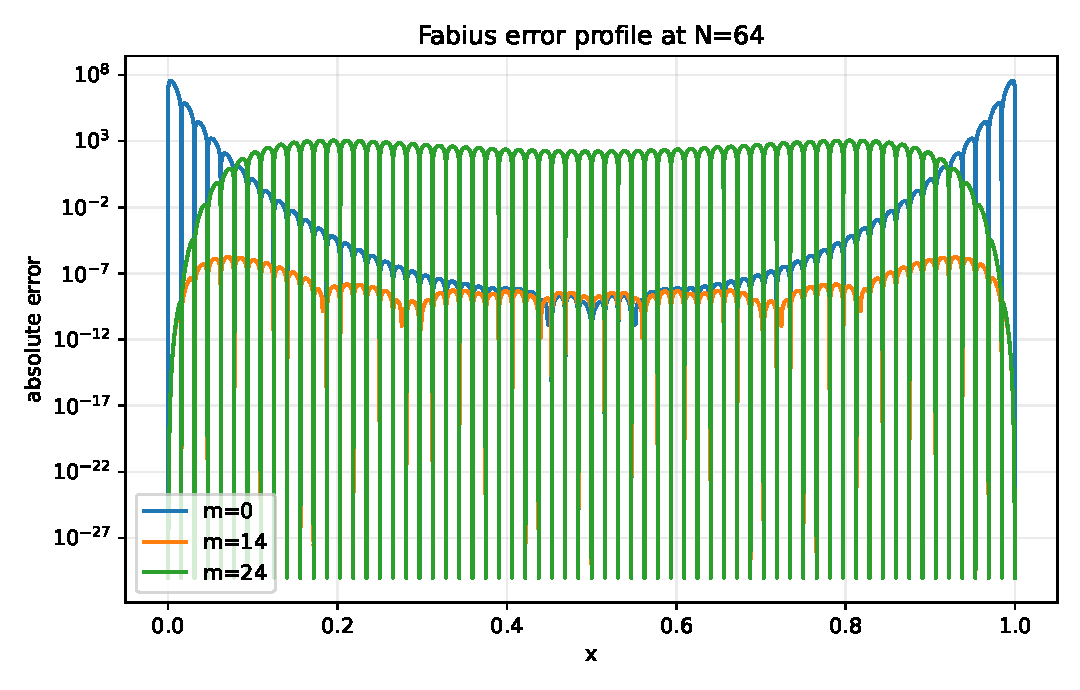
\includegraphics[width=0.86\textwidth]{fabius_error_profile_N64.pdf}
\caption{Absolute error profiles at $M=64$: the ordinary interpolant
($r=0$) with its giant boundary spike, the tuned order $r=14$, and
the overconstrained $r=24$ with the reverse instability emerging from
the center.  (Figure from the absorbed source with $N$ denoting the
comb size $M$.)}
\label{fig:error-profile}
\end{figure}

\begin{figure}[htbp]
\centering
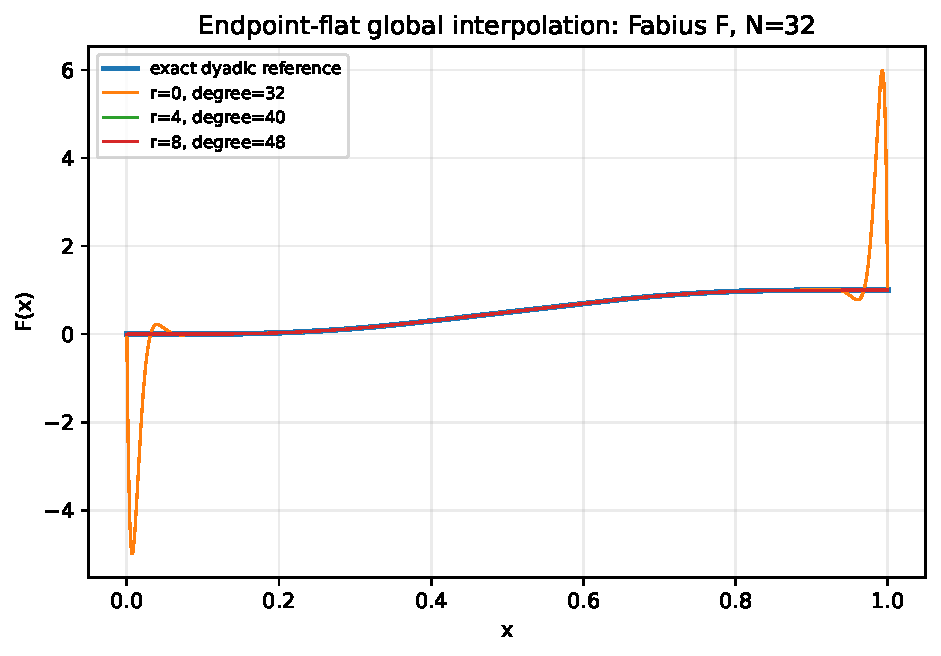
\includegraphics[width=0.80\textwidth]{fabius_N32_interpolants.pdf}
\caption{Fabius interpolation on the $M=32$ comb: ordinary
interpolation has entered the boundary-layer regime while moderate
endpoint jets recover excellent accuracy --- temporarily.}
\label{fig:F-N32}
\end{figure}

\begin{figure}[htbp]
\centering
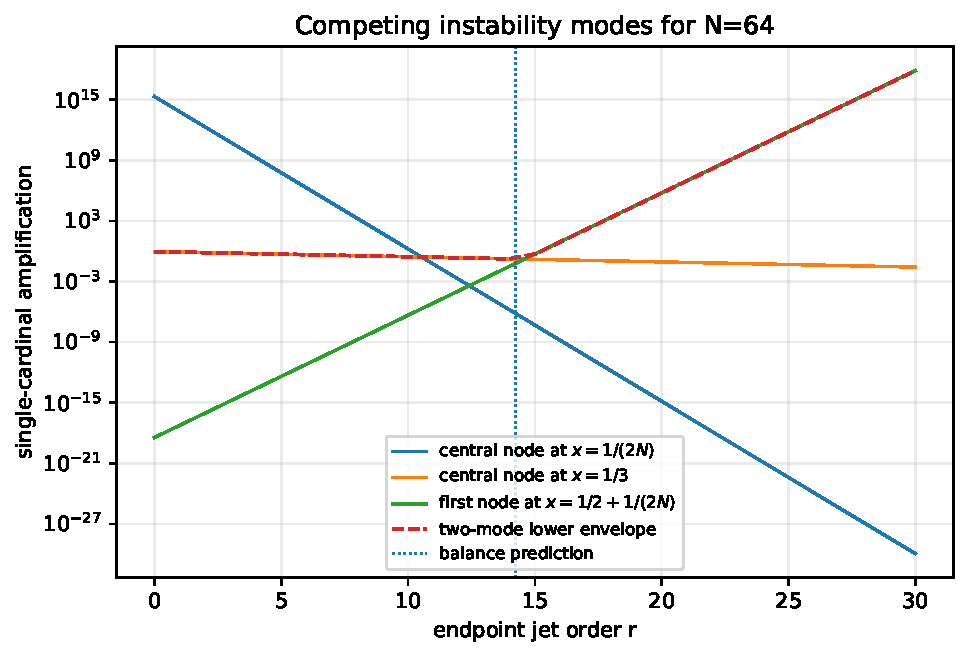
\includegraphics[width=0.80\textwidth]{cardinal_modes_N64.pdf}
\caption{The explicit value-cardinal modes at $M=64$ as functions of
the jet order: raising $r$ suppresses the boundary-to-center and
entropy modes but amplifies the first-interior-node mode; their
envelope --- the mechanism of \cref{thm:all-r} --- never becomes
small.}
\label{fig:cardinal-modes}
\end{figure}

\begin{figure}[htbp]
\centering
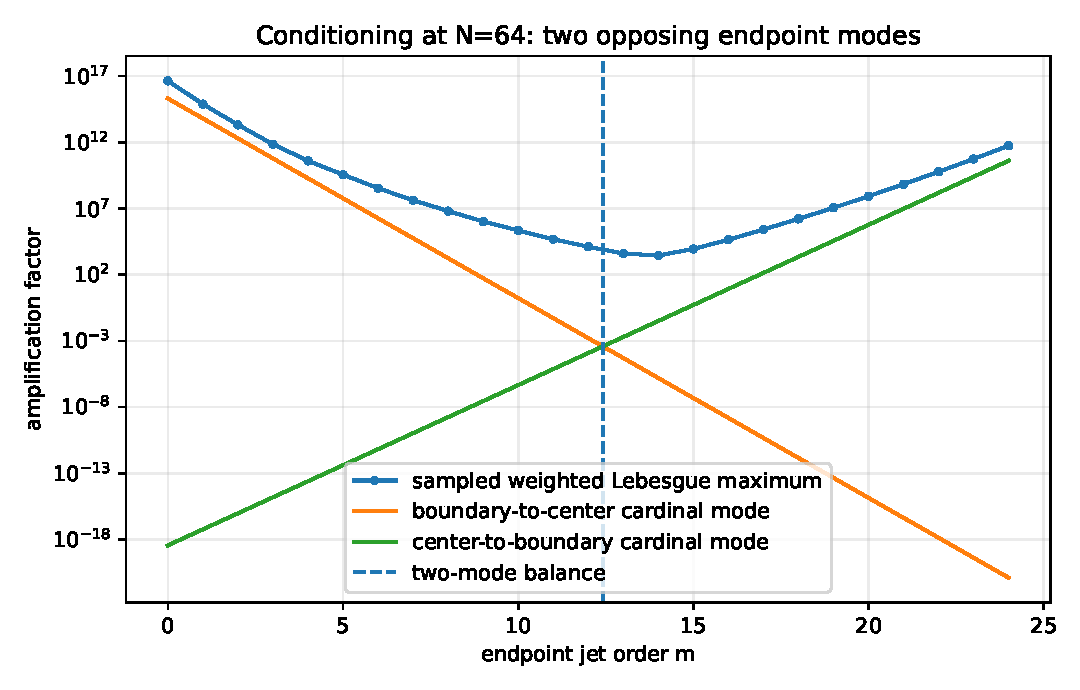
\includegraphics[width=0.80\textwidth]{conditioning_window_N64.pdf}
\caption{Sampled weighted Lebesgue maximum at $M=64$ against the two
exact mode lower bounds; their crossing predicts the useful
finite-$M$ window.}
\label{fig:conditioning-window}
\end{figure}

\begin{figure}[htbp]
\centering
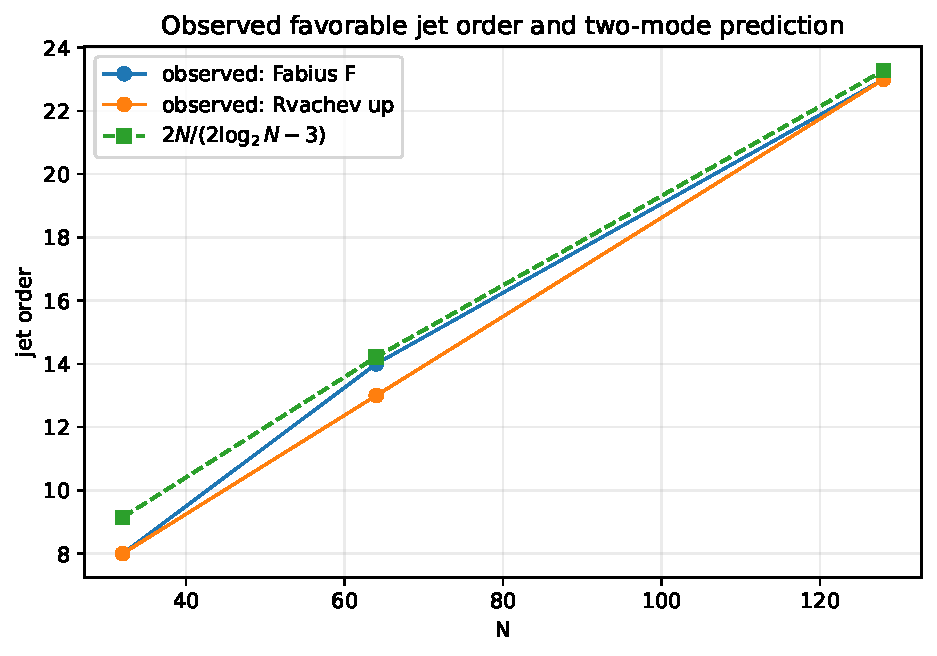
\includegraphics[width=0.78\textwidth]{balancing_law.pdf}
\caption{Observed optimal jet orders against the balance law
\eqref{eq:balance-log}.}
\label{fig:balance}
\end{figure}

\begin{figure}[htbp]
\centering
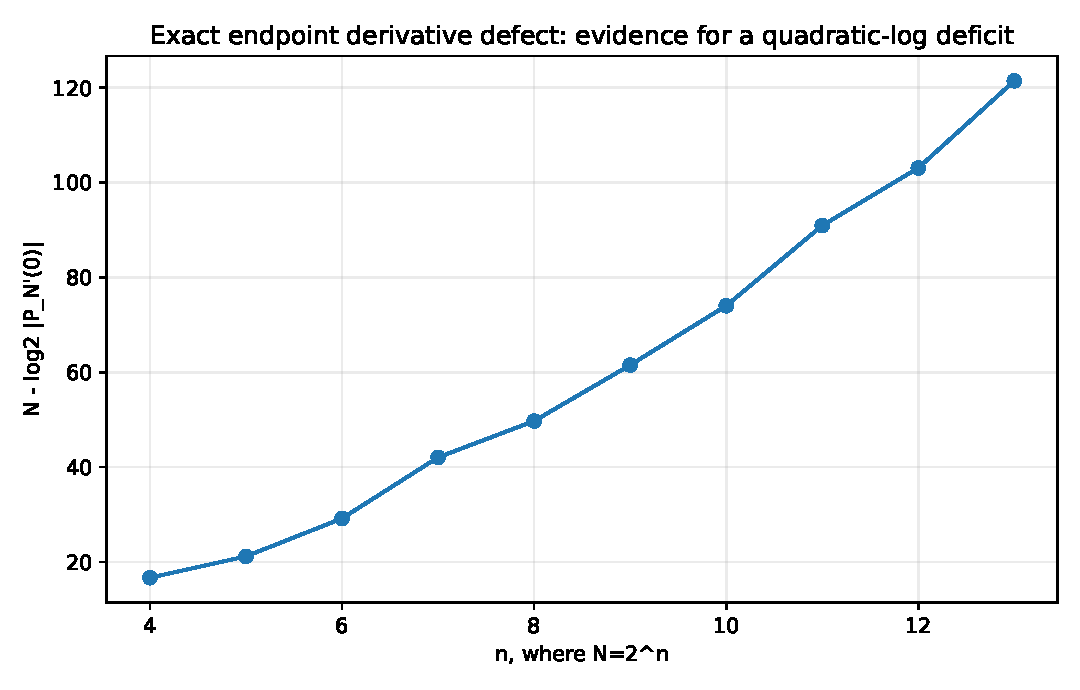
\includegraphics[width=0.82\textwidth]{endpoint_derivative_deficit.pdf}
\caption{The binary deficit $M-\log_2\abs{(P_M)'(0)}$ of
\cref{tab:derivative-defect}, consistent with a quadratic in
$\log_2M$ plus oscillation
(\cref{conj:derivative-law}).}
\label{fig:derivative-deficit}
\end{figure}

\subsection{Interpretation}

\begin{enumerate}
\item\emph{Runge behavior occurs for the specific functions}, not
merely for the operator: exact data, high precision, and refined
check grids leave the explosions unchanged.
\item\emph{Correct endpoint derivatives matter at finite $M$}: they
remove the first spurious jets \eqref{eq:jet-defect} and can improve
errors by factors up to $\sim10^{13}$.
\item\emph{The benefit has a finite window} of width
$\asymp M/(\log M)^{2}$, centered on the balance order; past it, the
$W_r(x_j)^{-1}$ amplification takes over, exactly as the mode
geometry predicts.
\item\emph{Function-specific cancellation is not stability}: at the
optimum the operator amplification is still $10^{3}$-scale at
$M=64$ and grows without bound; by $M=256$ no jet order helps.  The
cancellation that produces the $10^{-6}$ errors is a property of the
Thue--Morse structure of the exact samples --- understanding it is
the arithmetic frontier of \cref{sec:connections}.
\end{enumerate}

\section{The dyadic hierarchy and arithmetic connections}
\label{sec:connections}

\subsection{Nested corrections and the midpoint surplus}

Dyadic combs are nested, so successive interpolants differ by exactly
factorable corrections:
\begin{align}
 P_{2M}(x)-P_{M}(x)
 &=\omega_M(x)\,R_{M-1}(x),
 &\omega_M(x)&=\prod_{j=0}^{M}\Bigl(x-\frac jM\Bigr),
 \label{eq:nested-ordinary}\\
 H_{2M,r}(x)-H_{M,r}(x)
 &=\bigl[x(1-x)\bigr]^{r+1}
 \prod_{j=1}^{M-1}\Bigl(x-\frac jM\Bigr)\,R_{M-1,r}(x),
 \label{eq:nested-flat}
\end{align}
where in each case the quotient $R_{M-1,\cdot}\in\Pi_{M-1}$ is
determined by the $M$ \emph{midpoint surpluses}
\begin{equation}
 \sigma_{M,j}
 =F\!\left(\frac{2j+1}{2M}\right)
 -P_{M}\!\left(\frac{2j+1}{2M}\right)
 \qquad(\text{resp.\ }H_{M,r}),
 \label{eq:midpoint-surplus}
\end{equation}
by degree counting: both differences vanish at every coarse node (and
carry the endpoint multiplicities in the flat case), and the midpoint
values fix the quotient.  The surpluses are exact rationals, so the
hierarchy is a roundoff-free Runge diagnostic: a boundary surplus
whose normalized size grows signals the instability of the next level
before it is computed, and cells with small surpluses can stop
refining --- a mathematically transparent adaptive scheme specialized
to nested dyadic data.

\subsection{Thue--Morse cancellation and the mixed transform}

Every Newton coefficient $\Delta^{k}F(0)$ and every cardinal
evaluation is a finite signed sum of exact dyadic values, hence (by
\cref{thm:dyadic-values}) a finite Thue--Morse expression.  Prouhet
cancellation annihilates low-degree polynomial trends of complete
blocks --- the same mechanism as \cref{thm:Bell-Prouhet} --- which is
the structural reason the function-specific error near
$r_{\mathrm{bal}}$ can be so much smaller than the operator norm:
large cardinals meet blockwise signed moment identities in the data.
The cleanest single observable is the endpoint defect
\eqref{eq:endpoint-slope},
\begin{equation}
 D_M:=(P_M)'(0)
 =M\sum_{j=1}^{M}(-1)^{j-1}\binom Mj\frac{F(j/M)}{j}
 =M\int_0^1\sum_{j=1}^{M}(-1)^{j-1}\binom Mj
 F\!\left(\frac jM\right)t^{\,j-1}\dd t,
 \label{eq:mixed-transform}
\end{equation}
a \emph{mixed transform}: an ordinary ($q{=}1$) alternating Pascal row
applied to $q{=}\tfrac12$-structured data.  The integral form invites
a saddle analysis after inserting the exact evaluator; the entropy
concentration of the Pascal row near $j=M/2$, the Prouhet block
cancellation, the lower-Lambert endpoint scale of $F(j/M)$ for small
$j$, and a residual log-periodic phase all compete in
\cref{tab:derivative-defect}.  A rigorous asymptotic for
\eqref{eq:mixed-transform} would connect several currently separate
parts of the corpus and would settle
\cref{conj:derivative-law}.

The contrast between the two node geometries in the corpus is now
sharp:
\begin{center}
\small
\begin{tabular}{@{}lll@{}}
\toprule
Geometry & Nodes & Natural weights\\
\midrule
additive dyadic comb & $j/2^{m}$ & $(-1)^{j-1}\binom{M-2}{j-1}$
(2-adic law \eqref{eq:weight-valuation})\\
geometric/$q$ comb & $q^{j}$ or $-2^{j}$ & Gaussian-binomial products\\
\bottomrule
\end{tabular}
\end{center}
Both are Vandermonde inverses, over different node groups.  A mixed
transform interpolating across additive location while filtering
across dyadic scale --- for instance through the nested surplus
polynomials \eqref{eq:nested-flat} --- is a natural place to look for
an additive--multiplicative bridge; the valuation-selective filters of
\cref{sec:frontiers-sums} are the Part-I face of the same idea.

\subsection{Fourier, Lambert, and inverse-function connections}

\emph{Spectral view.}  A global polynomial has no localized Fourier
response: its boundary oscillation is broad spectral leakage.  A
cellwise operator (below) acts as a compactly supported
quasi-interpolant whose multiplier can be compared with the sinc
product \eqref{eq:Phi-product} near the origin --- a route to
sharpened local error constants that respects the compact-support
structure of $\Up$.

\emph{Lambert phases.}  The corpus's endpoint asymptotics carry a
nonconstant periodic correction in a lower-Lambert phase.  Three
observables here plausibly lock to it: the boundary-layer maximizer
(scale $1/M$ at $r=0$, \cref{conj:lambert-peak} in general), the
fluctuation $r_{\mathrm{opt}}-r_{\mathrm{bal}}$, and the log-periodic
component of the derivative-defect deficit
(\cref{conj:derivative-law}).

\emph{Inverse function.}  $F^{-1}$ has infinite endpoint
\emph{slopes}, the opposite pathology to flatness.  Direct equispaced
interpolation of $F^{-1}$ must fail at least as badly, and the
endpoint-flat machinery does not transfer; the natural schemes are
parametric interpolation of the exact pairs $(F(j/M),j/M)$, a
Lambert-coordinate transformation that removes the known singular
asymptotic before interpolating the slowly varying correction, or
monotone local rational/Hermite methods.  The Part-I comb calculus
faces the same issue for $\sum x_k^{p}F^{-1}(x_k)$
(\cref{sec:frontiers-sums}).

\section{Stable reconstruction on the same comb}
\label{sec:alternatives}

The negative results concern one global polynomial whose degree grows
with the sample count.  The same exact samples support provably
stable schemes; the global/local contrast is the practical conclusion
of Part II.

\subsection{Local Hermite interpolation: the cure}

For $s\ge0$ let $\mathcal H^{\mathrm{loc}}_{M,s}f$ be the piecewise
polynomial of degree $2s+1$ matching $f^{(k)}$, $0\le k\le s$, at both
ends of every cell $[j/M,(j+1)/M]$ --- all data exact rationals via
the derivative tower.

\begin{theorem}[Local Hermite error, with exact Fabius constants]
\label{thm:local-error}
For $f\in C^{2s+2}$,
\begin{equation}
 \norm{f-\mathcal H^{\mathrm{loc}}_{M,s}f}_\infty
 \le\frac{\norm{f^{(2s+2)}}_\infty}{(2s+2)!}
 \left(\frac{1}{4M^{2}}\right)^{s+1};
 \label{eq:local-general}
\end{equation}
in particular, inserting \eqref{eq:derivative-tower},
\begin{equation}
 \boxed{\;
 \norm{F-\mathcal H^{\mathrm{loc}}_{M,s}F}_\infty
 \le\frac{2^{(s+1)(2s+1)}}{(2s+2)!}\;M^{-2s-2},
 \qquad
 \norm{\Up-\mathcal H^{\mathrm{loc}}_{M,s}\Up}_\infty
 \le\frac{2^{\binom{2s+3}{2}}}{(2s+2)!}\;M^{-2s-2},
 \;}
 \label{eq:local-F-bound}
\end{equation}
the second bound for $M$ equal cells on $[-1,1]$.  The local value
and derivative cardinals have norms bounded independently of $M$: the
scheme is uniformly stable.
\end{theorem}

\begin{proof}
On a cell of length $h_0$ the two-point Hermite remainder is
$f^{(2s+2)}(\xi)\,(x-a)^{s+1}(x-b)^{s+1}/(2s+2)!$, bounded by
$(h_0^{2}/4)^{s+1}$ times the derivative norm.  For $F$, $h_0=1/M$
and the factor $4^{-(s+1)}$ lowers the derivative exponent
$\binom{2s+3}2$ to $(s+1)(2s+1)$; for $\Up$ on $[-1,1]$, $h_0=2/M$
makes $h_0^{2}/4=M^{-2}$ with no extra power of two.  Rescaling any
cell to $[0,1]$ shows the local cardinal basis depends only on $s$.
\end{proof}

With exact values and exact derivatives ($s=1$, cubic case) the
predicted $M^{-4}$ convergence is observed cleanly:
\begin{center}
\small
\begin{tabular}{@{}rrrrrr@{}}
\toprule
$M$ & 4 & 8 & 16 & 32 & 64\\
\midrule
sampled error & $9.67\times10^{-4}$ & $5.03\times10^{-4}$
 & $2.06\times10^{-5}$ & $2.29\times10^{-6}$ & $1.58\times10^{-7}$\\
\bottomrule
\end{tabular}
\captionof{table}{Piecewise-cubic Hermite errors for $F$
(level-$12$ check grid): steady algebraic convergence on the very
samples where the global polynomial explodes.}
\label{tab:local-errors}
\end{center}

\begin{figure}[htbp]
\centering
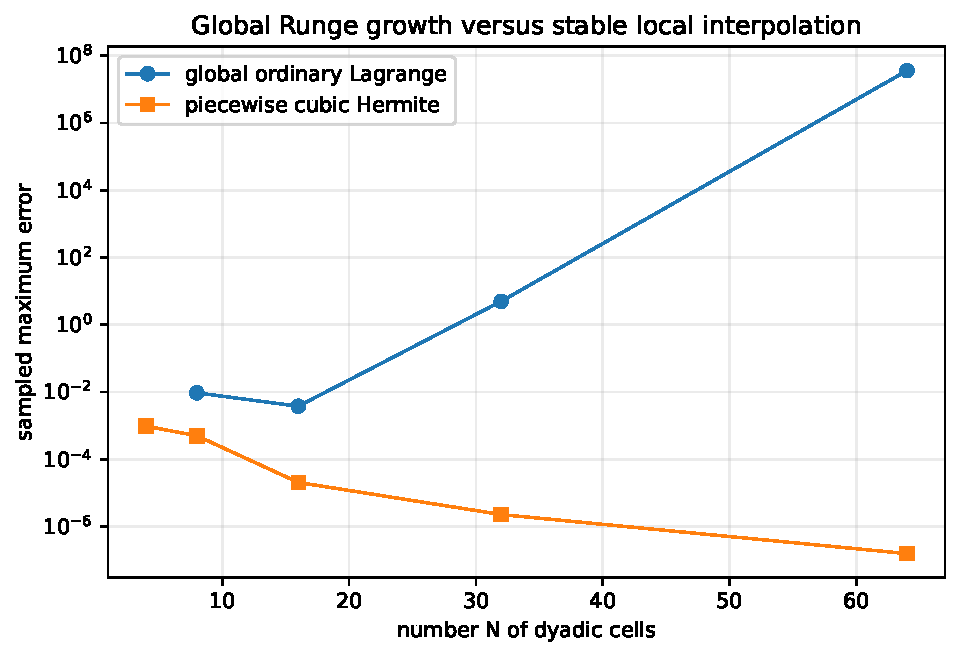
\includegraphics[width=0.80\textwidth]{global_vs_local.pdf}
\caption{Global ordinary interpolation versus the cellwise cubic
method on identical dyadic samples.}
\label{fig:global-local}
\end{figure}

\subsection{The wider menu}

Between the failed global extreme and the local cure lies a hierarchy
of methods that keep the exact dyadic data:

\begin{itemize}
\item\emph{Oversampled least squares.}  Fit degree $d\asymp\sqrt M$
to all $M+1$ samples, optionally imposing exact endpoint flatness
through the factorization \eqref{eq:H-def} with $Q$ fitted rather
than interpolated: stable root-exponential accuracy is the best
compatible with equispaced data
\cite{PlatteTrefethenKuijlaars2011,AdcockShadrin2023}.
\item\emph{Mock-Chebyshev subset interpolation.}  Interpolate only on
the comb points nearest to Chebyshev nodes, or constrain a
least-squares fit to them; constrained mock-Chebyshev methods extend
to Hermite data \cite{DellAccio2025}, for which the dyadic derivative
tower supplies exact samples.
\item\emph{Rational barycentric families.}  Floater--Hormann
interpolants have logarithmic Lebesgue growth on equispaced nodes
\cite{FloaterHormann2007,CirilloHormann2019}, and rational Hermite
variants accept the exact derivative data; applying them to the
deflated quotient $g_r$ preserves endpoint flatness exactly.
\item\emph{Mapped and Lambert coordinates.}  Interpolate in a
coordinate that respects $x\leftrightarrow1-x$ and opens the
endpoint scale --- a Lambert coordinate fitted to the known endpoint
asymptotics being the natural non-generic choice
(cf.\ Kosloff--Tal-Ezer maps).
\item\emph{Atomic/multiresolution bases.}  Expand in scaled
translates of $\Up$ itself (the refinement equation makes the dyadic
recursion exact), or in Faber--Schauder/spline systems --- the
representation-theoretic route developed elsewhere in the corpus,
with certified local error control.
\item\emph{Constrained minimax.}  Impose
$p(0)=0$, $p(1)=1$, $p^{(q)}(0)=p^{(q)}(1)=0$ and minimize the
residual on the comb in a stable basis for $g_r$.
\end{itemize}

\begin{statusbox}{Practical hierarchy}
(1) exact dyadic evaluation for data;
(2) local piecewise/atomic reconstruction for stability;
(3) global approximation only with degree well below the sample count
or after a change of basis/geometry;
(4) full-degree global interpolation only for small $M$ or as an
exact symbolic identity --- never as an asymptotic approximation
scheme.
\end{statusbox}

\section{Conjectures and frontier problems for Part II}
\label{sec:conjectures-interp}

The proved landscape is: operator instability at every jet order
(\cref{thm:fixed-r,thm:all-r,thm:global-hermite}), exact structural
identities (\cref{thm:factorization}, \cref{prop:modes},
\cref{thm:weight-valuation}), and a stable local alternative
(\cref{thm:local-error}).  The open frontier concerns the
\emph{specific} Fabius data.  Besides
\cref{conj:runge-divergence,conj:derivative-law,conj:higher-hermite,conj:lambert-peak}:

\begin{conjecture}[Optimal jet order]
\label{conj:optimal-r}
Let $r^{F}_M$ and $r^{\Up}_M$ minimize the true uniform errors of the
endpoint-flat families, and let $r^{\Leb}_M$ minimize
$\Leb_{M,r}$.  All three satisfy
\begin{equation}
 r_M=\frac{M\log2}{\log M}\bigl(1+\smallo(1)\bigr),
 \qquad\text{indeed}\qquad
 r_M=r_{\mathrm{bal}}(M)+\bigO\!\left(\frac{\log M}{\log\log M}\right),
 \label{eq:optimal-r-conj}
\end{equation}
with a stronger $\bigO(1)$ version along phase-locked dyadic
subsequences.  (Scanned data: \cref{tab:balance}.)
\end{conjecture}

\begin{conjecture}[Optimized divergence]
\label{conj:optimized-divergence}
$E^{*}_M:=\min_{r\ge0}\norm{F-H_{M,r}}_\infty$ does not tend to zero;
more strongly $\log E^{*}_M$ is eventually linear in $M$ up to
$\smallo(M)$, and for the Rvachev version
$\limsup E^{*,\Up}_M=+\infty$.  The measured sequence
$7.6\times10^{-7}\to1.8\times10^{-6}\to4.0\times10^{-3}
\to9.3\times10^{8}$ at $M=32,64,128,256$
(\cref{tab:optimized}) is the evidence; a proof must show the
Thue--Morse cancellation cannot keep pace with the exponential
envelope of \cref{thm:all-r}.
\end{conjecture}

\begin{conjecture}[Boundary-layer profile]
\label{conj:boundary-profile}
Along a dyadic subsequence there are normalizations $A_M$ with
$A_M\bigl(P_M(\xi/M)-F(\xi/M)\bigr)\to\mathcal E(\xi)$ locally for
$\xi>0$, the profile governed jointly by the entropy saddle of the
uniform cardinals and the lower-Lambert endpoint asymptotic of $F$.
\end{conjecture}

\begin{conjecture}[Surplus arithmetic]
\label{conj:surplus}
After clearing the natural common denominator
\eqref{eq:DeltaN}, the midpoint surplus vector
$(\sigma_{M,j})_j$ of \eqref{eq:midpoint-surplus} factors as a finite
binomial transform of a Thue--Morse block; its sign changes and its
largest boundary entries obey a depth-$m$ recursion.  (This would
make the nested hierarchy of \cref{sec:connections} an arithmetic
object and is the most concrete route to
\cref{conj:runge-divergence}: showing a boundary surplus cannot stay
small at all dyadic levels.)
\end{conjecture}

\begin{conjecture}[$2$-adic stability counterpart]
\label{conj:2adic-stability}
The valuation law \eqref{eq:weight-valuation} admits a renormalized
$2$-adic interpolation operator on the dyadic data with polynomially
bounded norm growth --- the archimedean catastrophe and the $2$-adic
regularity of the same weights being two valuations of one object.
Identify the correct Mahler-type basis and compare with the Newton
form \eqref{eq:newton-forward}.
\end{conjecture}

\begin{problem}[Noise threshold]
For tuned $r=r_{\mathrm{bal}}(M)$, quantify the largest relative
perturbation of the exact samples that preserves the observed
accuracy.  The crude bound $\Leb_{M,r}^{-1}$ is pessimistic; the
structured condition number should project noise onto the
self-similar residual subspace.
\end{problem}

\begin{question}[Sign structure of the differences]
Do the signs or $2$-adic valuations of $\Delta^{k}F(0)$ follow a
Thue--Morse or $q$-binomial law along $M=2^{m}$?  Such a law would
control the cancellations in \eqref{eq:newton-forward} and could turn
\cref{conj:runge-divergence} into a lower-bound proof.
\end{question}

Three research routes toward the divergence conjectures, in
increasing ambition: (i) insert the exact evaluator into one selected
cardinal evaluation and exploit blockwise Thue--Morse cancellation
until a dominant term survives; (ii) run a two-variable saddle
analysis of $\Delta^{k}F(0)$ in $(k,m)$, Bernoulli--Bell corrections
included; (iii) prove the surplus recursion of
\cref{conj:surplus}.  On the constructive side, the corrected balance
expansion \eqref{eq:balance-all-orders} should be computed and tested
against exact minimizers at $M=512$ and $1024$, separately for $F$
and $\Up$.

\section{Lean formalization program for Part II}
\label{sec:lean-interp}

The new results separate cleanly into finite algebra, exact gamma
identities, and elementary asymptotics --- a good match for the
repository's formalization style.  In dependency order:

\begin{enumerate}
\item\emph{Comb combinatorics}: nodes, barycentric weights, the
$2$-adic law \eqref{eq:weight-valuation}, symmetry and degree drop
(\cref{prop:symmetry}), Newton form and the Stirling jet transform
\eqref{eq:jet-defect}.
\item\emph{Endpoint-flat algebra}: the smoothstep
\eqref{eq:smoothstep} as a finite polynomial with its jet and
symmetry properties; divisibility by $W_r$; existence, uniqueness,
and the error identity of \cref{thm:factorization}.
\item\emph{Cardinal identities}: the finite-product forms of
\cref{lem:gamma-cardinal} and the exact modes
\eqref{eq:A-mode}--\eqref{eq:one-third-mode} as factorial/binomial
identities (gamma notation as corollaries).
\item\emph{Instability}: explicit Stirling bounds for factorials; the
two-regime dichotomy of \cref{thm:all-r}; the Hermite squares of
\cref{thm:global-hermite}.
\item\emph{Local stability}: the two-point Hermite remainder and the
derivative-norm specialization \eqref{eq:local-F-bound}.
\item\emph{Exact certificates}: kernel-checked rational error values
at small $M$ (as statements about finite grids, not continuum
suprema), and the exact endpoint defects of
\cref{tab:derivative-defect}.
\end{enumerate}

A natural module decomposition:
\begin{center}
\small
\begin{tabular}{@{}ll@{}}
\toprule
Module & Contents \\
\midrule
\nolinkurl{DyadicCombLagrange} & nodes, weights, symmetry, Newton form, $2$-adic law \\
\nolinkurl{EndpointFlatHermite} & smoothstep, factorization, uniqueness, error identity \\
\nolinkurl{WeightedLebesgue} & perturbation operator, cardinal functions \\
\nolinkurl{DyadicCombModes} & exact $A$/$B$/entropy-mode identities \\
\nolinkurl{DyadicCombInstability} & fixed-$r$ and all-$r$ exponential lower bounds \\
\nolinkurl{FabiusInterpolationDefect} & exact endpoint derivative transform \\
\nolinkurl{LocalHermiteStability} & cellwise remainder and Fabius constants \\
\bottomrule
\end{tabular}
\end{center}
This would extend the corpus's geometric-node Lagrange formalization
to the additive comb without duplicating it; the Part-I roadmap
(\cref{sec:frontiers-sums}) shares the first module.

\appendix

\section{Gamma-product calculations}
\label{app:gamma}

\subsection{Half-cell central cardinal (mode A)}
In the scaled variable $y=Mx$ with interior nodes $1,\dots,M-1$ and
$j=M/2$, at $y=\tfrac12$:
$\prod_{k=1}^{M-1}\abs{k-\tfrac12}=\Gamma(M-\tfrac12)/\Gamma(\tfrac12)$;
deleting the $j$ factor divides by $\abs{j-\tfrac12}=\tfrac M2-\tfrac12$,
and the denominator of the cardinal is
$(j-1)!\,(M-1-j)!=\Gamma(M/2)^{2}$, giving $A_M$ in
\eqref{eq:A-mode}.  The weight ratio is
$\bigl[\tfrac1{2M}(1-\tfrac1{2M})\bigr]/\tfrac14=(2M-1)/M^{2}=a_M$.
Stirling gives $A_M\sim2^{M}/(\pi\sqrt2\,M)$.

\subsection{Near-central boundary-node cardinal (mode B)}
For $j=1$ at $y=(M+1)/2$ with $M=2K$:
$\abs{\prod_{k=2}^{M-1}(y-k)}
=\bigl[\Gamma(K-\tfrac12)/\Gamma(\tfrac12)\bigr]^{2}$
(the products on the two sides of the half-integer are equal), and
the denominator is $(M-2)!=\Gamma(M-1)$, giving $B_M$.  The weight
ratio is
$\bigl[(\tfrac12+\tfrac1{2M})(\tfrac12-\tfrac1{2M})\bigr]
/\bigl[\tfrac1M(1-\tfrac1M)\bigr]=(M+1)/4=b_M$.  The duplication
formula turns $B_M$ into
$\dfrac{2^{2-M}}{\sqrt\pi}\,
\dfrac{\Gamma((M-1)/2)}{\Gamma(M/2)}
\sim2^{2-M}\sqrt{2/(\pi M)}$; equivalently
$B_M=\binom{M-2}{M/2-1}\big/16^{\,M/2-1}$.

\subsection{The one-third mode}
At $y=M/3$ (dyadic $M$ is never divisible by $3$):
$\prod_{k=1}^{M-1}(M/3-k)=\Gamma(M/3)/\Gamma(1-2M/3)$, and reflection
gives $1/\abs{\Gamma(1-2M/3)}
=\Gamma(2M/3)\abs{\sin(2\pi M/3)}/\pi
=\tfrac{\sqrt3}{2\pi}\Gamma(2M/3)$.  Removing the central factor
$\abs{M/3-M/2}=M/6$ and dividing by $\Gamma(M/2)^{2}$ gives
\eqref{eq:one-third-mode}; the exponential part of the gamma ratio is
$\exp\{M[\tfrac13\log\tfrac13+\tfrac23\log\tfrac23-\log\tfrac12]\}
=\e^{M(\log2-\Hyp(1/3))}$.

\subsection{Full-comb central cardinal}
For the full node set $0,\dots,M$ at $y=\tfrac12$, $j=M/2$:
$\prod_{k=0}^{M}\abs{\tfrac12-k}
=\tfrac12\,\Gamma(M+\tfrac12)/\Gamma(\tfrac12)$; deleting the
central factor divides by $\abs{\tfrac12-\tfrac M2}=\tfrac{M-1}2$,
and the denominator is
$(M/2)!\,(M/2)!=\Gamma(\tfrac M2+1)^{2}$, giving
\eqref{eq:full-central-cardinal}; Stirling's formula then yields
$\abs{\ell_{M/2}(\tfrac1{2M})}\sim\sqrt2\,2^{M}/(\pi M^{2})$, whose
square is \eqref{eq:hermite-square}.

\section{Mode asymptotics}
\label{app:mode-asymptotics}

Stirling's expansion in logarithmic form,
\begin{equation}
 \log\Gamma(z)
 =\Bigl(z-\tfrac12\Bigr)\log z-z+\tfrac12\log(2\pi)
 +\sum_{r=1}^{R-1}\frac{B_{2r}}{2r(2r-1)\,z^{2r-1}}
 +\bigO\bigl(z^{-2R+1}\bigr),
 \label{eq:stirling}
\end{equation}
applied to \eqref{eq:A-mode}--\eqref{eq:B-mode} yields
\begin{align}
 \log A_M&=M\log2-\log M-\log(\pi\sqrt2)+\bigO(M^{-1}),\\
 \log B_M&=-(M-2)\log2+\tfrac12\log\frac{2}{\pi M}+\bigO(M^{-1}),\\
 \log a_M&=-\log(M/2)+\log\bigl(1-\tfrac1{2M}\bigr),
 \qquad
 \log b_M=\log(M/4)+\log\bigl(1+\tfrac1M\bigr),
\end{align}
which prove \cref{prop:balance-asymptotic}.  Retaining further
Bernoulli terms and reverting with complete Bell polynomials yields
the all-orders program \eqref{eq:balance-all-orders}.

\section{Row reciprocity}
\label{app:row-symmetry}

With $A_m(z)=\sum_{k=0}^{M-1}F(k/M)z^{k}$ and
$F((M-k)/M)=1-F(k/M)$,
\begin{align}
 z^{M}A_m(1/z)
 &=\sum_{k=1}^{M}F\bigl((M-k)/M\bigr)z^{k}
 =\sum_{k=1}^{M}\bigl(1-F(k/M)\bigr)z^{k}
 =\frac{z(1-z^{M})}{1-z}-A_m(z)-z^{M},
\end{align}
which is \eqref{eq:AN-reciprocal}.  This exact reciprocity forces the
palindromic structure of the low-level row numerators
\eqref{eq:row-N1}--\eqref{eq:row-N3}.

\section{Core algorithms}
\label{app:algorithms}

\begin{lstlisting}[style=pythonstyle,caption={Streaming the exact
dyadic Fabius row (\cref{alg:stream}); \texttt{d} holds the exact
Fabius-law moments of \eqref{eq:d-recurrence}.}]
def fabius_row_exact(m):
    M = 2**m
    d = fabius_law_moments(m)          # Fractions d_0..d_m
    S = [0]*(m+1)                      # signed prefix power sums
    scale = Fraction(1, 2**(m*(m-1)//2) * factorial(m))
    row = []
    for a in range(M+1):
        row.append(scale * sum(comb(m,j)*d[j]*S[m-j]
                               for j in range(m+1)))
        if a == M: break
        eps = -1 if bin(a).count('1') % 2 else 1
        S = [S[0]+eps] + [sum(comb(k,q)*S[q] for q in range(k+1))
                          for k in range(1, m+1)]
    return row
\end{lstlisting}

\begin{lstlisting}[style=pythonstyle,caption={Endpoint-flat
interpolation in barycentric form (\cref{thm:factorization}).}]
S = lambda r,x: (factorial(2*r+1)//(factorial(r)**2)
                 * sum((-1)**k*comb(r,k)*x**(r+k+1)/(r+k+1)
                       for k in range(r+1)))
W = lambda r,x: (x*(1-x))**(r+1)
g = [(F(x_j)-S(r,x_j))/W(r,x_j) for x_j in interior_nodes]
w = [(-1)**(j-1)*comb(M-2,j-1) for j in range(1,M)]
H = S(r,x) + W(r,x)*barycentric(x, interior_nodes, g, w)
\end{lstlisting}

The absorbed packages add the sparse-difference row generation
($\bigO(mM)$), confluent divided differences for full-grid Hermite,
weighted-Lebesgue scans, and all figure/table generation; entry
points and reproduction commands are in each package's
\nolinkurl{README} under \nolinkurl{assets/}.

\section{Provenance of the absorbed sources}
\label{app:provenance}

This volume absorbs the following nine drafts (all dated 28 August
2026; SHA-256 of each main \texttt{.tex} source at absorption).  The
supporting material of each --- experiment scripts, CSV/data files,
figures, READMEs, and the sources' own SHA manifests --- is preserved
under \nolinkurl{assets/<directory>/}; the draft directories
themselves are deleted, git history being the archive.

\begin{center}
\small
\begin{tabular}{@{}p{0.44\textwidth}p{0.50\textwidth}@{}}
\toprule
Source (directory; SHA-256 prefix) & Role in this volume \\
\midrule
\emph{Dyadic-Comb Sums for the Fabius--Rvachev System}
(\nolinkurl{Fabius_Dyadic_Comb_Sums_Report_Package};
\texttt{4b6b0384df3f\ldots})
& Row OGF and pole collapse; Bernoulli--Thue--Morse and Bell--Prouhet
closed forms; the $\chi$-based collapse proof; odd-level defect
series; Hurwitz formula; Stirling reduction of iterated sums;
fractional-order semigroup; generated exact tables
(\cref{tab:integer-closed,tab:first-defects}). \\
\addlinespace
\emph{Dyadic-Comb Moments of the Fabius and Rvachev Functions}
(\nolinkurl{fabius-dyadic-comb-sums-report};
\texttt{b815be3b441e\ldots})
& Moment EGF; probabilistic Irwin--Hall proof of the dyadic
convolution; sparse $\bigO(mM)$ algorithm; one-sided transform;
spectral Dirichlet values $D(2),D(4)$ and their rationality;
midpoint identity; Newton fractional series; Richardson filtering;
tensor cubature. \\
\addlinespace
\emph{Dyadic-Comb Quadrature for the Fabius and Rvachev Functions}
(\nolinkurl{fabius_dyadic_comb_report_final};
\texttt{3379d821b764\ldots})
& Shifted exactness for arbitrary real phase; $2$-adic alias
hierarchy; Bell--Bernoulli jet calculus; parity threshold
$\tau(p)$ and the one-formula closed form; absolute integer powers;
cutoff-Mellin lemma, universal zeta correction, shifted Hurwitz
corrections, negative-power renormalization; iterated closed forms;
base-$b$ extension; phase-superconvergence experiments. \\
\addlinespace
\emph{Dyadic-Comb Interpolation of the Fabius and Rvachev Functions}
(\nolinkurl{fabius_dyadic_interpolation_report};
\texttt{970d261c4cb7\ldots})
& Streaming evaluator; symmetry compression; smoothstep
factorization; half-cell and one-third modes; fixed-$r$ theorem;
leading-log balance law; all-node Hermite theorem
($4^{M}/M^{4}$); nested corrections and midpoint surplus; local
Hermite stability theorem with exact constants; gamma appendix. \\
\addlinespace
\emph{Dyadic-Comb Interpolation of the Fabius and Rvachev Functions}
(independent write-up, same title;
\nolinkurl{fabius_interpolation_report};
\texttt{799ff356366\ldots})
& Bit-recursion evaluator; degree drop; exact finite-$M$ balance
order, window width, and thresholds; entropy-mode instability
proof; measured weighted Lebesgue constants; exact endpoint
derivative defects to $M=8192$ and the quadratic-log conjecture;
mixed $q{=}1/q{=}\tfrac12$ transform; Lambert budget inversion;
alternatives survey; Lean module table. \\
\addlinespace
\emph{Global Polynomial Interpolation of the Fabius and Rvachev
Functions on Dyadic Combs}
(\nolinkurl{Fabius_Rvachev_Dyadic_Interpolation_Report};
\texttt{f4d8c1c280ad\ldots})
& $2$-adic weight valuation law; exact error identity form of the
factorization; even reduction of the full Rvachev comb to quadratic
nodes; general confluent Hermite data and tables; $M=256$
optimized-divergence data; ordinary Lebesgue-constant measurements;
Lambert peak-migration saddle; mock-Chebyshev/rational-Hermite
survey and references. \\
\addlinespace
\emph{Euler--Maclaurin and Exhaustion Quadratures for Fabius and
Rvachev Moments} (tenth wave;
\nolinkurl{Fabius_Euler_Maclaurin_Report_Package};
\texttt{9ea76d14b863\ldots})
& The Bernoulli-periodization section \cref{sec:periodized}: shifted
corrected rules for general polynomial weights, composite-mesh
$2$-adic termination and reflection reduction, the phase-modulated
first-defect series and Fabius-side forced phases, the first-harmonic
positivity proof (\cref{thm:D-positive}, settling the former
spectral-positivity conjecture), the closed exhaustion tail and
derivative-free rational Richardson extraction, base-$b$ dichotomy,
composite-mesh Rvachev quadrature, the Thue--Morse moment-identity
family, and the mesh/phase/analytic-weight frontier items.
Deduplicated: the corpus background, the dyadic endpoint collapse and
its threshold (= \cref{thm:EM-collapse} route), the odd-level defect
series and spectral rationality
(= \cref{thm:odd-defect,thm:D-rational}), the leading-jet lemma, the
dyadic shifted Rvachev quadrature (= \cref{thm:shifted-exactness}),
and the phase-superconvergence parity pattern. \\
\addlinespace
\emph{Exhaustion, Euler--Maclaurin, and Spectral Exactness for
Fabius--Rvachev Monomial Integrals} (eleventh wave;
\nolinkurl{fabius_rvachev_exhaustion_euler_maclaurin_bundle};
\texttt{7ba2cb99a591\ldots})
& The tenth-wave report's independently written twin, merged into
\cref{sec:periodized}: the exact all-mesh alias--Bernoulli identity
\eqref{eq:all-mesh} (layer cake + Faulhaber; no threshold), the
general-$q$ first defect in Bernoulli-moment and spectral forms
\eqref{eq:general-q-defect} with midpoint/upper parity
superconvergence one level below threshold, the Bernoulli moments
$\beta_{2m}=\E B_{2m}(Y)$ with the spectral identity
\eqref{eq:beta-D} (whose sign law, conjectured by the twin, follows
from \cref{thm:D-positive} --- \cref{cor:beta-sign}), the
one-correction half-interval Rvachev rule \eqref{eq:half-up-rule}
with the termination/one-mode exhaustion dichotomy and two-level
recovery, the supergeometric odd-base bound, variable mesh chains,
and the $q=\tfrac14$ Gaussian-binomial filter form.  Deduplicated:
the telescoping exhaustion frame, the corrected shifted rule and its
$\vtwo(M)>d$ threshold, the dyadic first defect, the $F$-side Ruffa
tails, the base-$b$ dichotomy skeleton, the Thue--Morse moment
family, and the full-support Rvachev quadrature (all already present
from the tenth wave or the volume core). \\
\addlinespace
\emph{Bernoulli--Ruffa Phase--Resolution Calculus for Fabius and
Rvachev Moment Integrals} (twelfth wave;
\nolinkurl{fabius_ruffa_phase_calculus};
\texttt{064180a4b44c\ldots})
& Third member of the periodization circle, audited against the
consolidated volumes themselves.  Kept: the multiple-angle domination
lemma $\abs{\Phi(q\ell/2)}\le\abs{\Phi(q/2)}/\ell$
(\cref{lem:multiple-angle}) with the twisted-positivity theorem
\cref{thm:twisted-D-positive} and the complete phase zero-set theorem
\cref{thm:phase-zero-set} (settling the Rvachev- and Fabius-side
phase-classification conjectures and the former twisted-positivity
question, uniformly in the odd part); finite phase cubature
\cref{thm:phase-cubature} with dyadic rational certificates; the
phase--resolution separation principle; the Thue--Morse--Bernoulli
generating function \cref{thm:tm-bernoulli-egf} with exact digital
phase filters, root-of-unity and general digit-mask generalizations;
coherent radix exhaustion along tag orbits $\{b^N\alpha\}$; exact
anisotropic tensor shells; the full-support transfer formula for
$I_p$; the proved all-orders complex-$\alpha$ expansion
\eqref{eq:complex-alpha-EM}; and the minimal-phase, double-scaling,
and automatic-filter frontier items.  Deduplicated: the master
shifted identity and $2$-adic collapse, open/midpoint forms, the
first-defect series and forced phases, exact Ruffa layers/tails,
even-radix layers, $q$-extrapolation (kept as a remark in its
general-phase form), and the full-support cubature. \\
\bottomrule
\end{tabular}
\end{center}

\emph{What was deduplicated.}  All six sources restate the corpus
background of \cref{sec:foundations}; the three sums sources prove
the same collapse theorem (three routes; the $\chi$-aliasing proof is
presented here, the operator-identity and one-sided-transform routes
surviving as \eqref{eq:g0-hat} and remarks) and the same first-defect
series in three normalizations; the three interpolation sources prove
the same factorization theorem, the same fixed-order instability, and
three variants of the all-order instability (the entropy-mode proof
is presented here; the $x=\tfrac13$ and $a=\tfrac1{10}$ variants
survive as the exact identity \eqref{eq:one-third-mode} and the
choice of $a$ in the proof).  Their numerical tables overlap heavily
and agree wherever they overlap; each retained table cites its
generating package.  The two new exact values $D(6),D(8)$ of
\eqref{eq:D-values} were computed for this volume as described in
\cref{sec:dirichlet}.  Beyond notation, no source's mathematical
content was discarded.

Each source carried its own audit of the repository corpus against
duplication (pinned snapshots from
\texttt{fa53516a\ldots} to \texttt{3c7f2912\ldots}); their unanimous
conclusion --- no prior additive-comb Runge study, no endpoint-flat
factorization, no unweighted-comb collapse theorem in the audited
corpus --- is inherited here, with the same caveat that this is a
corpus-relative and targeted-literature novelty standard, not a claim
of universal priority.

\begin{thebibliography}{99}

\bibitem{Fabius1966}
J.~Fabius,
\newblock A probabilistic example of a nowhere analytic
$C^\infty$-function,
\newblock \emph{Zeitschrift f\"ur Wahrscheinlichkeitstheorie und
Verwandte Gebiete} \textbf{5} (1966), 173--174.
DOI: \nolinkurl{10.1007/BF00536652}.

\bibitem{Jessen1935}
B.~Jessen and A.~Wintner,
\newblock Distribution functions and the Riemann zeta function,
\newblock \emph{Transactions of the American Mathematical Society}
\textbf{38} (1935), 48--88.

\bibitem{Rvachev1971}
V.~L.~Rvachev and V.~A.~Rvachev,
\newblock A certain finite function,
\newblock \emph{Dopovidi Akademii Nauk Ukrains'koi RSR, Series A}
(1971), 705--707, 764.

\bibitem{Rvachev1990}
V.~A.~Rvachev,
\newblock Compactly supported solutions of functional-differential
equations and their applications,
\newblock \emph{Russian Mathematical Surveys} \textbf{45} (1990),
no.~1, 87--120.

\bibitem{Arias1982}
J.~Arias de Reyna,
\newblock Definici\'on y estudio de una funci\'on indefinidamente
diferenciable de soporte compacto,
\newblock \emph{Revista de la Real Academia de Ciencias Exactas,
F\'isicas y Naturales de Madrid} \textbf{76} (1982), no.~1, 21--38;
English translation arXiv:\nolinkurl{1702.05442} (2017).

\bibitem{AriasArithmetic}
J.~Arias de Reyna,
\newblock Arithmetic of the Fabius function,
\newblock \emph{INTEGERS} \textbf{18} (2018), Article A51;
arXiv:\nolinkurl{1702.06487}, version 3.

\bibitem{Haugland2016}
J.~K.~Haugland,
\newblock Evaluating the Fabius function,
\newblock arXiv:\nolinkurl{1609.07999} (2016).

\bibitem{AlloucheShallit}
J.-P.~Allouche and J.~Shallit,
\newblock \emph{Automatic Sequences: Theory, Applications,
Generalizations},
\newblock Cambridge University Press, 2003.

\bibitem{Comtet}
L.~Comtet,
\newblock \emph{Advanced Combinatorics},
\newblock Reidel, 1974.

\bibitem{GKP}
R.~L.~Graham, D.~E.~Knuth, and O.~Patashnik,
\newblock \emph{Concrete Mathematics}, 2nd ed.,
\newblock Addison--Wesley, 1994.

\bibitem{NIST}
F.~W.~J.~Olver et al.\ (eds.),
\newblock \emph{NIST Digital Library of Mathematical Functions},
\newblock \nolinkurl{https://dlmf.nist.gov/}; chapters on Bernoulli
polynomials, Hurwitz zeta, and asymptotic expansions.

\bibitem{StrangFix}
G.~Strang and G.~Fix,
\newblock A Fourier analysis of the finite element variational
method,
\newblock in \emph{Constructive Aspects of Functional Analysis},
C.I.M.E., 1973, pp.~793--840.

\bibitem{deBoorRon}
C.~de~Boor and A.~Ron,
\newblock Fourier analysis of the approximation power of principal
shift-invariant spaces,
\newblock \emph{Constructive Approximation} \textbf{8} (1992),
427--462.

\bibitem{TrefethenWeideman2014}
L.~N.~Trefethen and J.~A.~C.~Weideman,
\newblock The exponentially convergent trapezoidal rule,
\newblock \emph{SIAM Review} \textbf{56} (2014), no.~3, 385--458.

\bibitem{Navot1961}
I.~Navot,
\newblock An extension of the Euler--Maclaurin summation formula to
functions with a branch singularity,
\newblock \emph{Journal of Mathematics and Physics} \textbf{40}
(1961), 271--276.

\bibitem{BerlineVergne}
N.~Berline and M.~Vergne,
\newblock Local asymptotic Euler--Maclaurin expansion for Riemann
sums over a semi-rational polyhedron,
\newblock arXiv:\nolinkurl{1502.01671} (2015).

\bibitem{BuchheitKessler}
A.~A.~Buchheit and T.~Ke{\ss}ler,
\newblock Singular Euler--Maclaurin expansion,
\newblock arXiv:\nolinkurl{2003.12422} (2020).

\bibitem{Runge1901}
C.~Runge,
\newblock \"Uber empirische Funktionen und die Interpolation
zwischen \"aquidistanten Ordinaten,
\newblock \emph{Zeitschrift f\"ur Mathematik und Physik}
\textbf{46} (1901), 224--243.

\bibitem{Mills1992}
T.~M.~Mills and S.~J.~Smith,
\newblock The Lebesgue constant for Lagrange interpolation on
equidistant nodes,
\newblock \emph{Numerische Mathematik} \textbf{61} (1992), 111--115.

\bibitem{Brutman1997}
L.~Brutman,
\newblock Lebesgue functions for polynomial interpolation --- a
survey,
\newblock \emph{Annals of Numerical Mathematics} \textbf{4} (1997),
111--127.

\bibitem{Smith2006}
S.~J.~Smith,
\newblock Lebesgue constants in polynomial interpolation,
\newblock \emph{Annales Mathematicae et Informaticae} \textbf{33}
(2006), 109--123.

\bibitem{BerrutTrefethen2004}
J.-P.~Berrut and L.~N.~Trefethen,
\newblock Barycentric Lagrange interpolation,
\newblock \emph{SIAM Review} \textbf{46} (2004), no.~3, 501--517.

\bibitem{Higham2004}
N.~J.~Higham,
\newblock The numerical stability of barycentric Lagrange
interpolation,
\newblock \emph{IMA Journal of Numerical Analysis} \textbf{24}
(2004), 547--556.

\bibitem{CoppersmithRivlin1992}
D.~Coppersmith and T.~J.~Rivlin,
\newblock The growth of polynomials bounded at equally spaced
points,
\newblock \emph{SIAM Journal on Mathematical Analysis} \textbf{23}
(1992), no.~4, 970--983.

\bibitem{PlatteTrefethenKuijlaars2011}
R.~B.~Platte, L.~N.~Trefethen, and A.~B.~J.~Kuijlaars,
\newblock Impossibility of fast stable approximation of analytic
functions from equispaced samples,
\newblock \emph{SIAM Review} \textbf{53} (2011), no.~2, 308--318.

\bibitem{Trefethen2013}
L.~N.~Trefethen,
\newblock \emph{Approximation Theory and Approximation Practice},
\newblock SIAM, Philadelphia, 2013.

\bibitem{Manni1993}
C.~Manni,
\newblock Lebesgue constants for Hermite and Fej\'er interpolation on
equidistant nodes,
\newblock \emph{Calcolo} \textbf{30} (1993), 93--102.

\bibitem{FloaterHormann2007}
M.~S.~Floater and K.~Hormann,
\newblock Barycentric rational interpolation with no poles and high
rates of approximation,
\newblock \emph{Numerische Mathematik} \textbf{107} (2007),
315--331.

\bibitem{CirilloHormann2019}
E.~Cirillo and K.~Hormann,
\newblock On the Lebesgue constant of barycentric rational Hermite
interpolants at equidistant nodes,
\newblock \emph{Journal of Computational and Applied Mathematics}
\textbf{349} (2019), 143--155.

\bibitem{AdcockShadrin2023}
B.~Adcock and A.~Shadrin,
\newblock Fast and stable approximation of analytic functions from
equispaced samples via polynomial frames,
\newblock \emph{Constructive Approximation} \textbf{57} (2023),
257--294.

\bibitem{DellAccio2025}
F.~Dell'Accio, F.~Marcell\'an, and F.~Nudo,
\newblock Constrained mock-Chebyshev least squares approximation for
Hermite interpolation,
\newblock \emph{Numerical Algorithms} (2025),
DOI: \nolinkurl{10.1007/s11075-025-02051-7}.

\bibitem{Corless1996}
R.~M.~Corless, G.~H.~Gonnet, D.~E.~G.~Hare, D.~J.~Jeffrey, and
D.~E.~Knuth,
\newblock On the Lambert $W$ function,
\newblock \emph{Advances in Computational Mathematics} \textbf{5}
(1996), 329--359.

\bibitem{Flajolet1995}
P.~Flajolet, X.~Gourdon, and P.~Dumas,
\newblock Mellin transforms and asymptotics: harmonic sums,
\newblock \emph{Theoretical Computer Science} \textbf{144} (1995),
3--58.

\bibitem{ProveItPrimary}
V.~Reshetnikov,
\newblock \emph{The Fabius Function and Rvachev's Up-Function},
\newblock primary exposition in the \texttt{ProveIt} repository,
\repo, snapshot 28 August 2026.

\bibitem{ProveItFrontier}
V.~Reshetnikov,
\newblock \emph{Non-Formalized Research Frontiers for the Fabius
Function},
\newblock \texttt{ProveIt} repository, \repo, snapshot 28 August
2026.

\end{thebibliography}

\end{document}
